\documentclass[a4paper,dvipdfmx,reqno,12pt]{amsart}
\synctex=1
%
%%%% packages
\usepackage[utf8]{inputenc}
\usepackage[dvipdfmx]{graphicx,color}%for images
\usepackage{bm}%fonts
\usepackage{tikz-cd}%
\usetikzlibrary{cd}
\usetikzlibrary{calc}
\usepackage{amsmath,amsthm,amstext,amsfonts,amsbsy}% ほぼ必須
\usepackage{amssymb}
\usepackage{latexsym}% ほぼ必須
\usepackage{makecell}%表のセル内で改行するためのパッケージ
\usepackage{algpseudocode,algorithm}%疑似コード用
\usepackage{todonotes}%comments
\usepackage[margin=0.8in]{geometry}
\usepackage{layout}
\usepackage[T1]{fontenc}%font encoding
\usepackage{physics}
\usepackage{braket}%after physics
\usepackage{mathtools,thmtools}
\usepackage{imakeidx}%before hyperref for pagebackref
\usepackage[pagebackref,dvipdfmx]{hyperref}
\usepackage[capitalize]{cleveref}
\hypersetup{
     colorlinks = true,
     citecolor  = blue,
     linkcolor  = blue, 
     urlcolor   = blue, 
}
%\usepackage{pxjahyper}%for hyperref in Japanese
\usepackage{bookmark}
\usepackage{dynkin-diagrams}

%%%% imakeidx
\makeindex
\makeindex[name=not, title=Index, columns=2]
\makeindex[name=sym, title=Symbol, columns=3]
\makeindex[name=ref, title=Ref, columns=3]

\newcommand{\ind}[2]{\emph{#1}\index{1{#2}@{#1}}}
\newcommand{\indset}[3]{$#1 \deq #2 $ \index{0{#3}@$#1$} }
\newcommand{\indse}[2]{{$#1$}\index{0{#2}@{$#1$}}}

%%%%
\usepackage{pgf,tikz,pgfplots}
\pgfplotsset{compat=1.15}
\usetikzlibrary{arrows}



%%%%


%%%% theoremstyle

\theoremstyle{definition}
\newtheorem{theorem}{Theorem}[section]
\newtheorem*{theorem*}{Theorem}
\newtheorem{definition}[theorem]{Definition}
\newtheorem{definition*}{Definition}
\newtheorem{example}[theorem]{Example}
\newtheorem*{example*}{Example}
\newtheorem{proposition}[theorem]{Proposition}
\newtheorem*{proposition*}{Proposition}
\newtheorem{Note}[theorem]{Note}
\newtheorem*{Note*}{Note}
\newtheorem{Ntc}[theorem]{Notice}
\newtheorem*{Ntc*}{Notice}
\newtheorem{lemma}[theorem]{Lemma}
\newtheorem*{lemma*}{Lemma}
\newtheorem{Fact}[theorem]{Fact}
\newtheorem*{Fact*}{Fact}
\newtheorem{question}[theorem]{Question}
\newtheorem*{question*}{Question}
\newtheorem{conjecture}[theorem]{Conjecture}
\newtheorem*{conjecture*}{Conjecture}
\newtheorem{Rule}[theorem]{Rule}
\newtheorem*{Rule*}{Rule}
\newtheorem{notation}[theorem]{Notation}
\newtheorem*{Not*}{Notation}
\newtheorem{corollary}[theorem]{Corollary}
\newtheorem*{corollary*}{Corollary}
\newtheorem{remark}[theorem]{Remark}
\newtheorem*{Rmk*}{Remark}
\newtheorem{condition}[theorem]{Condition}
\newtheorem*{condition*}{Condition}
\newtheorem{Conv}[theorem]{Convention}
\newtheorem*{Conv*}{Convention}
\newtheorem{observation}[theorem]{Observation}
\newtheorem*{observation*}{Observation}
%%%% newcommand

%%%logic symbol
\newcommand{\deq}{\coloneqq}

\newcommand{\dbraket}[1]{\hspace{-1.5pt}\braket{\hspace{-2.2pt}\braket{#1}\hspace{-2.2pt}}}

\newcommand{\textcmd}[1]{\texttt{\symbol{"5C}#1}}

%%special sets
\newcommand{\emp}{\varnothing}%emptyset
\newcommand{\C}{\mathbb{C}}%complex number
\newcommand{\Ha}{\mathbb{H}}%quaternion
\newcommand{\F}{\mathbb{F}}%field
\newcommand{\R}{\mathbb{R}}%real number
\newcommand{\Q}{\mathbb{Q}}%rational number
\newcommand{\Z}{\mathbb{Z}}%integer
\newcommand{\N}{\mathbb{N}_{0}}%natural number
\newcommand{\Pj}{\mathbb{P}}%bold p
\newcommand{\vep}{\varepsilon}%varepsilon

%%%%

\newcommand{\mb}[1]{\mathbb{#1}}%blackboard bold (for math mode)
\newcommand{\mcal}[1]{\mathcal{#1}}%

\newcommand{\opn}[1]{\operatorname{#1}}
\newcommand{\catn}[1]{\mathbf{#1}}

\newcommand{\abk}[1]{\langle {#1} \rangle}%angle bracket 
\newcommand{\Abk}[1]{\left \langle {#1} \right \rangle}%angle bracket (auto sizing)
\newcommand{\dabk}[1]{\langle\! \langle {#1}\rangle \! \rangle}%double angle bracket
\newcommand{\Dabk}[1]{\left \langle \! \left \langle {#1} \right \rangle \! \right \rangle}%double angle bracket
\newcommand{\Sbk}[1]{\left[ {#1} ]\right }% square bracket [] (auto sizing)
\newcommand{\Cbk}[1]{\left \{ {#1}\right \}}% curly bracket {} (auto sizing)
\newcommand{\dcbk}[1]{\{\!\!\{ {#1}\}\!\!\}} % double curly bracket {{}} 
\newcommand{\Dcbk}[1]{\left \{\!\! \left \{ {#1} \right\} \!\!\right \}} % double curly bracket {{}} (auto sizing)
\newcommand{\Paren}[1]{\left ( {#1} \right )}%parenthesis () (auto sizing)
\newcommand{\dparen}[1]{(\!({#1})\!)}%double parenthesis
\newcommand{\xto}[1]{\xrightarrow{#1}}
\newcommand{\xgets}[1]{\xleftarrow{#1}}
\newcommand{\hookto}{\hookrightarrow}


%%%% 

%%%% mathabx.sty (font) 
\DeclareFontFamily{U}{matha}{\hyphenchar\font45}
\DeclareFontShape{U}{matha}{m}{n}{
      <5> <6> <7> <8> <9> <10> gen * matha
      <10.95> matha10 <12> <14.4> <17.28> <20.74> <24.88> matha12
      }{}
\DeclareSymbolFont{matha}{U}{matha}{m}{n}

\DeclareFontFamily{U}{mathb}{\hyphenchar\font45}
\DeclareFontShape{U}{mathb}{m}{n}{
      <5> <6> <7> <8> <9> <10> gen * mathb
      <10.95> mathb10 <12> <14.4> <17.28> <20.74> <24.88> mathb12
      }{}
\DeclareSymbolFont{mathb}{U}{mathb}{m}{n}

\DeclareFontFamily{U}{mathx}{\hyphenchar\font45}
\DeclareFontShape{U}{mathx}{m}{n}{
      <5> <6> <7> <8> <9> <10>
      <10.95> <12> <14.4> <17.28> <20.74> <24.88>
      mathx10
      }{}
\DeclareSymbolFont{mathx}{U}{mathx}{m}{n}

%DeclareMathSymbol (from mathabx.sty)
\DeclareMathSymbol{\bigboxslash}{\mathop}{mathx}{"FE}
\DeclareMathSymbol{\bigboxtimes}{\mathop}{mathx}{"D2}
%%%%

%%%% MnSymbol.sty (font)
\DeclareFontFamily{U}{MnSymbolC}{}
\DeclareFontShape{U}{MnSymbolC}{m}{n}{
  <-6> MnSymbolC5
  <6-7> MnSymbolC6
  <7-8> MnSymbolC7
  <8-9> MnSymbolC8
  <9-10> MnSymbolC9
  <10-12> MnSymbolC10
  <12-> MnSymbolC12}{}
\DeclareFontShape{U}{MnSymbolC}{b}{n}{
  <-6> MnSymbolA-Bold5
  <6-7> MnSymbolC-Bold6
  <7-8> MnSymbolC-Bold7
  <8-9> MnSymbolC-Bold8
  <9-10> MnSymbolC-Bold9
  <10-12> MnSymbolC-Bold10
  <12-> MnSymbolC-Bold12}{}

\DeclareSymbolFont{MnSyC}{U}{MnSymbolC}{m}{n}

%%%% DeclareMathSymbol (from MnSymbol.sty)

\DeclareMathSymbol{\tplus}{\mathbin}{MnSyC}{43}
\DeclareMathSymbol{\aplus}{\mathbin}{MnSyC}{190}

%%%% renewcommand




%%%% footnote

\newcommand{\cfootnote}[1]{\footnote{#1}}

\newcommand{\myfootnote}[1]{\hspace{-5pt}\footnote{#1}}

\newcommand{\TB}{\mcal{T}_{B_0}}
\newcommand{\TBZ}{\mcal{T}_{\Z,B_0}}
\newcommand{\AffS}{{\mathop{\mcal{A}\!f\!\!f\!}\nolimits}}
\newcommand{\FBZ}{\mcal{F}_{\Z,B}}
\newcommand{\FB}{\mcal{F}_{B}}
\newcommand{\simto}{ 
\mathrel{\raisebox{0.13em}{${\sim}$}}
\kern -0.75em \mathrel{\raisebox{-0.11em}{${\scriptstyle \to}$}}  
}
%%%% from 

%%%% from  https://tex.stackexchange.com/questions/183702/formatting-back-references-in-bibliography-bibtex
\renewcommand*{\backrefalt}[4]{
    \ifcase #1 [Not cited.]%
        \or        [Cited on p.#2.]%
        \else      [Cited on p.#2.]%
    \fi}


\usepackage{mathrsfs}
\usepackage{upgreek}
\numberwithin{equation}{section}
\title{On counting lattice points in some tropical spaces and beyond
}
\author[Y. Tsutsui]{Yuki Tsutsui}
\address{Graduate School of Mathematical Sciences,
The University of Tokyo, 3-8-1 Komaba, Meguro-Ku,
Tokyo, 153-8914, Japan}
\email{tyuki@ms.u-tokyo.ac.jp}
\date{\today}

\begin{document}

\begin{abstract}
We consider a tropical analog of Euler characteristic 
of line bundles of algebraic varieties for compact
boundaryless tropical manifolds by using inspired
ideas from Strominger--Yau--Zaslow conjecture 
and Morse theory.
As a test play, we prove a certain analog of 
Riemann--Roch formula for compact tropical curves 
and integral affine manifolds with a Hessian form.
Our analog is different from tropical Riemann--Roch
theorem that proved by Gathmann--Kerber.
\end{abstract}
\maketitle
\section{Introduction}
%TODO: 日本語で4000字の論文の要旨

Tropical geometry is a combinatorial and convex 
geometrical analog of
algebraic geometry or analytic geometry.
Some typical tropical variety comes from 
a subvariety $X$ of an algebraic split torus 
$(K^{\times})^{n}$
by tropicalization $\opn{Trop}(X)$ of $X$.
$\opn{Trop}(X)$ is an $\dim X$-dimensional 
polyhedral complex satisfying a certain 
balancing condion
(see for instance 
\cite[Theorem 3.2.3]{MR3287221}).

The tropical Riemann--Roch theorem for a 
divisor $D$ of tropical curves $C$ is proved 
by Gathemann--Kerber \cite{gathmannRiemannRochTheoremTropical2008a}
as an extension of Riemann--Roch theorem for graphs
\cite{MR2355607} (see also 
\cite{mikhalkinTropicalCurvesTheir2008a}) as 
the following equation: 

\begin{align}
r(D)-r(K_C-D)=\opn{deg}(D)+\chi_{\opn{top}}(C)
\end{align}


The Hirzebruch--Riemann--Roch theorem (HRR for short) and 
the Grothendieck--Riemann--Roch theorem (GRR for short) 
are monumental works in
algebraic geometry (or complex geometry). 
Here is the statement of HRR for holomorphic line bundles on 
projective complex manifolds.
\begin{theorem}[{\cite{MR0202713}}]
Let $X$ be a compact projective complex manifold and
$\mathcal{L}$ a holomorphic line bundle on $X$.
Then there exists the following equation:
\begin{align} \label{equation-HRR}
\chi(H^{\bullet}(X;\mathcal{L}))
=\int_X \opn{ch}(\mathcal{L})\opn{td}(X).
\end{align}
\end{theorem}

The HRR is generalized for 
general compact complex 
manifolds as a corollary of Atiyah--Singer index 
theorem.

Since the Euler number of line bundle is invariant for 
degeneration of varieties
\myfootnote{
For instance, let $X\to \opn{Spec}(\Z_{p})$ be a
projective scheme over $\Z_{p}$ and $\mcal{L}$
be a line bundle on $X$ that is flat over $\Z_{p}$.
Then, 
$\chi_{\kappa(s)}(X_s;\mcal{L}_s)=
\chi_{\kappa(\eta)}(X_{\eta};\mcal{L}_{\eta})$.
Roughly speaking, this means that
we can calculate the Euler number of line bundles on
a projective scheme of characteristic zero from that on a 
projective scheme of a positive characteristic.
}
(e.g. \cite[p.50]{MR2514037}), 
and thus we can expect calculate (or estimate)
the Euler number of many interesting line bundles
by the geometry of dual complex of degeneration 
for a good family of algebraic variety or 
tropicalization.

Besides, we can also consider the following question:

\begin{question} \label{question-tropical-euler}
What is a tropical analog of Euler number of sheaf 
cohomology of line bundles on algebraic varieties for 
tropical spaces? Is there some analogs of HRR or GRR 
for tropical varieties?
\end{question}

This is the main topic of our paper.
In particular, we mainly focus on
the former question.


However, tropical Riemann--Roch theorem 
for tropical varieties has been proved yet 
as a generalization of 
\cite{gathmannRiemannRochTheoremTropical2008a}.

However, there exist various difficulties for 
\cref{question-tropical-euler} by root causes of 
tropical geometry.

One of main difficulty for \cref{question-tropical-euler} 
is that line bundles on tropical spaces are not sheaves of 
Abelian groups but commutative monoids in general.
For more detail about the previous related results of 
tropical Riemann--Roch theorem
and more difficulties for 
\cref{question-tropical-euler}, see 
\cref{section-tropical-riemann-roch}.

On the other hand, we can get the following 
observation from a great deal of studies:
\begin{observation} \label{observation-tropical-euler}
The Euler characteristic of the structure sheaf of 
tropical manifold should be equal to 
the topological Euler characteristic of it.
\end{observation}
See \cref{remark-list-tropical-euler} for the reason of 
\cref{observation-tropical-euler}. 
The obervation gives a hint for
\cref{question-tropical-euler}.  







In this paper, we pursue a different tropical
analog of Euler number of line bundles with the help of 
ideas on toric varieties, Morse theory,
Strominger--Yau--Zaslow conjecture
(SYZ conjecture for short), geometric prequantization
and related topics.

\begin{remark}
\label{remark-todd-class}
We note about the RHS of \cref{equation-HRR} 
for tropical manifolds. 
The $1$-st Chern class $c_1(\mathcal{L})$ of 
tropical line bundle $\mathcal{L}$ and 
the Chow group of rational polyhedral spaces and 
its cycle map is 
well-studied \cite{gross2019sheaftheoretic},
and thus we can define the Chern character
$\opn{ch}(\mathcal{L})$ of 
$\mathcal{L}$ naturally.
On the other hand, the Todd class of tropical manifold
have not been studied well enough yet  
when the dimension of tropical manifold is greater
than $2$.
We won't discuss the general theory of Todd class of tropical 
manifolds in this paper, 
but should be essentially defined from the theory of 
Chern--Schwartz--MacPherson cycles for matroids 
\cite[Previous work]{lopezdemedranoChernSchwartzMacPhersonCyclesMatroids2020}.
See also \cite[5.3]{mikhalkinTropicalGeometryIts2006} and
\cite[Definition 3.20]{shawTropicalSurfaces2015a}.
\end{remark}

\subsection{Counting lattice point of lattice polytopes}
In this subsection, we explain some backgrounds of 
our approach of our definition of Euler characteristic
of tropical line bundles.

In the case of some special line bundles on
tropical toric variety, our definition of Euler 
characteristic of tropical line bundle is essentially same with the
number of lattice points of the lattice polytope of it.

Before explaining about it, we recall some 
elemental properties of projective toric varieties over 
$\mathbb{C}$.
((See also \cite{MR2810322} for fundamental
properties of classical toric varieties.))
Let $P$ be a $n$-dimensional lattice polytope in 
$\mathbb{R}^{n}$, $X_P$ the projective toric variety
of $P$, $\mathcal{L}_P$ the line bundle on 
$X_P$ of $P$.
The sheaf cohomology of $\mathcal{L}_P$ has 
the following explicit isomorphisms:
\begin{align}
H^{\bullet}(X_P;\mathcal{L}_P)=
H^{0}(X_P;\mathcal{L}_P)\simeq
\bigoplus_{u\in P\cap \mathbb{Z}^{n}} \mathbb{C}z^{u},
\label{equation-danilov-formula} \\
H^{\bullet}(X_P;\mathcal{L}_P^{\vee})=
H^{n}(X_P;\mathcal{L}_P^{\vee})\simeq 
\bigoplus_{u\in \opn{int}(P)\cap \mathbb{Z}^{n}}\mathbb{C}z^{u}.
\end{align}
In particular, we have
\begin{align} \label{equation-ehrhart-reciprocity}
\chi(H^{\bullet}(X;\mathcal{L}_P))=
\sharp (P\cap \mathbb{Z}^{n}), \quad 
\chi(H^{\bullet}(X;\mathcal{L}_P^{\vee}))=
\sharp (\opn{int}(P)\cap \mathbb{Z}^{n}).
\end{align}
By \cref{equation-danilov-formula}, we can interpret HRR 
for smooth toric varieties 
as follows:
\begin{align}
\label{equation-toric-HRR}
\sharp (P\cap \mathbb{Z}^{n})
=\int_{X_P}\opn{ch}(\mathcal{L}_P)\opn{td}(X_P).
\end{align}
The prototype slogan of our approach
for a tropical analog of HRR is 
a realization of \cref{equation-toric-HRR}
for tropical manifolds.
We also note \cref{equation-danilov-formula} 
has a differential geometrical interpretation,
see also \cref{appendix-geometric-quantization}. 


Next, we will interpret the LHS of 
\cref{equation-toric-HRR} by the language
of tropical toric varieties.
\myfootnote{
In \cite{MR4155409},
new Ehrhart theory of tropical geometry appear, 
but this is different from our approach.
}
In this paper, we mainly use max-plus algebra for 
tropical geometry.


Basic concepts and properties 
of tropical toric varieties is studied and 
explained in \cite{MR2428356,MR2511632,meyer2011intersection,MR3287221}.
Let $P$ be an $n$-dimensional convex lattice polytope in
$(\mathbb{R}^{n})^{\vee}$ and
$f\colon \mathbb{R}^{n} \to \mathbb{R}$ a 
smooth function which is defined as follows:
\begin{align}
  f(x)\deq\log (\sum_{u\in P\cap (\mathbb{Z}^{n})^{\vee}} 
\opn{exp}(a_u+\abk{u,x})),\quad  (a_u\in \mathbb{R}).
\label{equation-log-polynomial} 
\end{align}
Here 
$\abk{\cdot,\cdot}\colon 
(\mathbb{R}^{n})^{\vee}\times \mathbb{R}^{n}\to\mathbb{R}$
is the canonical pairing of a vector space and its dual.

We note $f$ is a Laurent polynomial function over the 
log semiring. 
In fact, $f=\opn{log}\circ p\circ \opn{exp}$ 
for some polynomial 
$p\in \mathbb{R}_{\geq 0}[x_1^{\pm},\ldots,x_n^{\pm}]
\setminus \{0\}$ over the semifield of nonnegative
real numbers and $\opn{log}$ is a semifield isomorphism
from definition.
This observation is well-known and important 
for our approach.
Let $x_1,\ldots,x_n$ be the standard coordinates of 
$\mathbb{R}^{n}$.
The differential
$df:{\mathbb{R}}^{n}\to ({\mathbb{R}}^{n})^{\vee}; x\mapsto 
(\frac{\partial f}{\partial x_1}(x),\ldots,\frac{\partial f}{\partial x_n}(x))$ 
is an embedding onto the (relative) interior of $P$
\cite[p.124 Exercise]{MR1301331}. 
The differential map is also naturally appeared as an 
exponential family in algebraic statistic,
information geometry and Hessian geometry.
\begin{example}
Let $f\colon \mathbb{R} \to {\mathbb{R}}; x\mapsto \log (1+e^{x})$ be a soft 
plus function. When we take a dequantization of $f$,
we get a ReLU $f^{\opn{trop}}(x)=\max\{0,x\}$ which 
is frequently used in machine learning.
The differential is a sigmoid function 
$df(x)=\frac{e^{x}}{1+e^{x}}$ and 
the image of $df$ is the open interval $(0,1)$.
\myfootnote{
The softmax function also are appeared 
naturally in a similar way 
when we consider tropical projective spaces.}
\end{example}

From now on, we assume 
$a_u=1$ for all $u\in P\cap \mathbb{Z}^{n}$ for simplicity.
We can naturally extend $df$ on tropical projective toric 
varieties and then the extension map is called the \emph{tropical moment map}
$\mu_{P}^{\opn{trop}}: X_{P}^{\opn{trop}}\simto P$ 
\cite[Definition 2.1 (2)]{MR2428356}.
Instead of moment map for Hamiltonian action of Lie group on
symplectic manifold, we
need not assume convex lattice polytope is Delzant.
This is a tropical analog of algebraic moment map 
for toric varieties
(see for example
\cite[\textsection 12.2]{MR2810322}).

Let 
$q: ({\mathbb{R}}^{n})^{\vee}\to ({\mathbb{R}}^{n})^{\vee}/(\Z^{n})^{\vee}$ 
a canonical projection map.
Then the number of set of the intersection point of 
the graph of $q\circ \mu_P^{\opn{trop}}$ and 
that of zero map 
$0_{X_P^{\opn{trop}}}\colon X_P^{\opn{trop}} \to
({\mathbb{R}}^{n})^{\vee}/(\Z^{n})^{\vee}$ is equal to the 
number of lattice points in $P$:
\begin{align}
\label{equation-moment-map-intersection}
\sharp (0_{X_P^{\opn{trop}}}\cap q\circ\mu_P^{\opn{trop}})
=\sharp (P \cap \Z^{n}).
\end{align}
On the other hand, from \cref{equation-log-polynomial} 
we can construct data $\{(U_i,f_i)\}_{i\in I}$ of 
pairs of open subsets 
$U_i$ of $X_{P}^{\opn{trop}}$ and 
"smooth functions" $f_i\colon U_i \to \mathbb{R}$. 
The data is very similar with elements of 
$\opn{CaDiv}^{\infty}(X_{P}^{\opn{trop}})\deq H^{0}(X_{P}^{\opn{trop}};
\mcal{A}^{0,0}_{X_{P}^{\opn{trop}}}/
\mathcal{O}^{\times}_{X_{P}^{\opn{trop}}})$.
\myfootnote{
Be careful that this data is not an element
of $\opn{CaDiv}^{\infty}(X_{P}^{\opn{trop}})$ since
 the former collection of smooth functions is not constant
at any neighborhood of the corner of $X_{P}^{\opn{trop}}$,
i.e., the fixed point of the torus action on tropical 
toric varieties.
In particular, every (0,0)-superform on 
$\mathbb{T}^n$ is constant at 
$(-\infty,\ldots,-\infty)$.

By adding functions 
$\opn{log}\circ f \circ\opn{exp}$ for some smooth function
$f\colon \mathbb{R}_{\geq 0}^{n}\to \mathbb{R}_{>0}$,
we can overcome this weak point.
}
$\opn{CaDiv}^{\infty}(X_{P}^{\opn{trop}})$ is a
smooth version of the group of tropical Cartier divisor
$\opn{CaDiv}(X_{P}^{\opn{trop}})$ 
\cite[Definition 4.2]{MR3894860}
which is defined by the sheaf of $(0,0)$-super forms 
$\mcal{A}^{0,0}_X$ on 
polyhedral spaces.
\begin{example} \label{eg: TP1Cartier}
Fix a continuous function $f\colon \mathbb{R}\to \mathbb{R}; 
x\mapsto \opn{log}(1+e^{nx})$.
Its differential induces a homeomorphism 
from $\mathbb{T}P^1$ onto $[0,n]$. 
$\mathbb{T}P^{1}$ is covered by two open subsets:
$U_1\deq \mathbb{T}$ and $U_2\deq \mb{R}\cup\{+\infty\}$.
Take two continuous functions on each $U_i$ as follows:
\begin{align}
f_{1,n}\colon \mathbb{T}\to \mathbb{T};
x \mapsto \log (1+e^{nx}),\quad
f_{2,n}\colon \mb{R}\cup\{+\infty\} \to 
\mathbb{T};
x\mapsto \log(1+e^{nx})-nx.
\end{align}

Data $\{(U_i,f_{i,n})\}_{i=1,2}$ defines an element 
$D_n\deq (f_{1,n}-f_{2,n}=nx)\in 
H^{1}(\mb{T}P^1;\mcal{O}_{\mb{T}P^1}^{\times})\simeq \Z$
as a \v{C}ech cocycle.
Then, we have the following analog of 
\cref{equation-toric-HRR}:
\begin{align}
\label{equation-MRR-tropical-line}
\sharp([0,n]\cap \Z)=\opn{deg}(D_n)+1=
\opn{deg}(D_n)+\chi_{\opn{top}}(\mb{T}P^1).
\end{align}
\end{example}







%TODO: ラグランジュ切断に関して説明。

\subsection{Lagrangian sections and 
homological mirror symmetry}

Another important point is that 
we can consider the LHS of 
\cref{equation-moment-map-intersection}
as the intersection number 
of two "Lagrangian submanifolds".
We now explain about this meaning by
using the theory of integral affine manifolds.
An $n$-dimensional 
\emph{integral affine manifold} $B_0$ 
is a differential manifold 
with a fixed atlas whose transition maps is locally in 
$\opn{GL}(n,\mathbb{Z})\ltimes \mathbb{R}^{n}$.
Every integral affine manifold is a tropical manifold.
Historically, integral affine manifolds are 
deeply-studied in the field of symplectic geometry 
as a base space of Lagrangian torus fibration before
the terminology "tropical geometry" appear.

Every integral affine manifold $B_0$ has 
a canonical $\mathbb{Z}$-local system 
$\mathcal{T}^{\vee}_{\mathbb{Z},B_0}$ of integer
valued cotangent vectors. 
The integral affine structure of $B_0$ induces a
torus fibration 
$f\colon \colon T^{*}B_0/\mathcal{T}^{\vee}_{\mathbb{Z},B_0}
\to B_0$ and 
$T^{*}B_0/\mathcal{T}^{\vee}_{\mathbb{Z},B_0}$ has 
a standard symplectic structure induced from that of 
cotangent bundle $T^{*}B_0$.
We write $\check{X}(B_0)\deq 
T^{*}B_0/\mathcal{T}^{\vee}_{\mathbb{Z},B_0}$
Let $f\colon B\to \mathbb{R}$ be a 
smooth function on a smooth manifold $B$.
$f$ defines a section 
$\sigma_{df}\colon B\to T^{*}B; x\mapsto (x;df(x))$ of 
the cotangent bundle $\pi\colon T^{*}B\to B$.
We note that the intersection number of 
$\sigma_{df}$ and the zero section of the cotangent
bundle is equal to the topological Euler characteristic
of $B$ if $B$ is compact.
If $B$ is an integral affine manifold,
$\sigma_{df}$ induces a section 
$s_{df}\colon B\to T^*B/\Lambda$ of a torus fibration
$\check{\pi}_B\colon T^*B/\Lambda \to B$ via a canonical 
projection $\pi \colon T^*B\to T^*B/\Lambda$.
$T^{*}B_0$ and $\check{X}(B_0)\deq T^*B\to T^*B/\Lambda$
has a canonical symplectic structure and
both $\sigma_{df}(B)$ (resp. $s_{df}(B)$) are Lagrangian 
submanifolds of $T^{*}B_0$ 
(resp. $T^*B/\check{\Lambda}$).

\emph{Lagrangian sections} is a section 
$s\colon B_0\to \check{X}(B_0)$ such that 
$\opn{Im} s$ is a Lagrangian submanifolds.

\index{Lagrangian section@Lagrangian section}
which is well-studied in the field of homological 
mirror symmetry 
(see for instance \cite{MR1882331}).
In general, every element $D$ of Picard group of 
integral affine manifold $B$ has a smooth Cartier
divisor $s\in \opn{CDiv}^{\infty}(B)$ whose divisor 
class is equal to $D$ and 
$s$ induces a Lagrangian section of 
$\check{\pi}_{B_0}\colon \check{X}(B)\to B$.


\begin{example}
If $B$ is a tropical elliptic curve 
$\mathbb{R}/\mathbb{Z}$, then we can check there exists 
a similar formula of 
(\ref{equation-MRR-tropical-line}) easily.
Let $f_n\colon \mathbb{R}\to \mathbb{R};
x\mapsto \frac{n}{2}x^{2}$ be a quadratic polynomial.
The polynomial induces a smooth Cartier divisor 
$s_n$ on $\mathbb{R}/\mathbb{Z}$ naturally.
The associated Lagrangian section of $f_n$ is
$s_n'\colon\mathbb{R}/\mathbb{Z}\to 
\check{X}(\mathbb{R}/\mathbb{Z});x\mapsto (x;nx)$.
Then,
\begin{align}
\sharp(0_{\check{X}(\mathbb{R}/\mathbb{Z})}\cap 
s_n'(\mathbb{R}/\mathbb{Z}))
=\opn{deg}(s_n)+\chi_{\opn{top}}(\mathbb{R}/\mathbb{Z}). 
\end{align}
This is a certain analog of Riemann--Roch formula 
for elliptic curves.
\end{example}
The above example can be considered as a toy result 
of HMS conjecture and SYZ conjecture for 
Calabi--Yau manifolds.



\ind{Homological Mirror Symmetry}{Homological Mirror 
Symmetry} or \ind{HMS}{HMS} is a conjecture about 
categorical equivalence between two different 
triangulated category derived from symplectic geometry 
of Calabi-Yau manifold $\check{X}$ and complex geometry 
of a Calabi-Yau manifold $\mathcal{X}$ (or a degenerate family of 
Calabi-Yau manifold $X_t$) \cite{MR1403918}:
\myfootnote{One of important motivation of HMS 
is a solution of 
\ind{Classical Mirror Symmetry}{classical
mirror symmetry} 
which was appeared from string theory 
but we will not discuss about this 
since this solution is still an open question.}
\begin{align}
  \Phi \colon \opn{D}^{\pi}(\opn{Fuk}(\check{X}))\simeq 
\opn{D}^{b}(\opn{Coh}(\mathcal{X})).
\end{align}
The RHS is called the derived category of 
Fukaya category of $\check{X}$ and 
$\mathcal{X}$ is a Calabi--Yau manifold over 
the Novikov field $\Lambda^{\mathbb{C}}_{\mathrm{nov}}$ 
with $\mathbb{C}$-coefficients.
To our knowledge, the general definition 
of the Fukaya category of Calabi--Yau manifold
will be appeared in \cite{afooo}.
HMS induces an isomorphism between (Lagrangian) 
Floer cohomology of a pair of Lagrangian branes 
$(\mathscr{L}_0,\mathscr{L})$ and 
Ext group of coherent sheaves:
\begin{align} \label{equation-HMS-HF}
\opn{HF}^{\bullet}(\mathscr{L}_0,\mathscr{L})
\simeq  \opn{Ext}^{\bullet}_{\mcal{O}_{\mcal{X}}}
(\Phi(\mathscr{L}_0),\Phi(\mathscr{L})).
\end{align}

In partivcular, if $\Phi(\mathscr{L}_0)
  \simeq \mcal{O}_{\mathcal{X}}$ and 
$\Phi(\mathscr{L})$ is a line bundle on $\mathcal{X}$,
then we have the following equation 
from HMS and HRR:
\begin{align}
\label{equation-MRR}
\chi (\opn{HF}^{\bullet}(\mathscr{L}_0,\mathscr{L}))=
\int_{\mathcal{X}}\opn{ch}(\Phi(\mathscr{L}))
\opn{td}(\mathcal{X}).
\end{align}

Similar question is called 
Mirror Riemann--Roch conjecture in 
\cite[Conjecture 4.9]{grossSpecialLagrangianFibrations1998a}.

%TODO: SYZとは

\ind{Strominger-Yau-Zaslow conjecture}{Strominger-Yau-
Zaslow conjecture} or 
\ind{SYZ conjecture}{SYZ conjecture} is a conjecture 
in physics about 
a concrete method to solve Kontsevich's Homological 
Mirror Symmetry conjecture for Calabi-Yau manifolds
\cite{stromingerMirrorSymmetryTduality1996}.

((See also 
\cite[\textsection 1.3.2,
\textsection 7.3.7]{MR2567952} for more details about 
SYZ conjecture.))

SYZ conjecture gives a concrete method to create 
a $A_{\infty}$-functor 
$\Phi_{\mathrm{SYZ}}\colon 
\opn{Fuk}(\check{X})\to D^{b}(\opn{Coh}(
\mathcal{X}))$
which induces a quasi-equivalence
induces a quasi-equivalence 
$D^{\pi}(\opn{Fuk}(\check{X}))\simeq 
D^{b}(\opn{Coh}(\mathcal{X}))$.

Under assumption of SYZ conjecture, 
every Lagrangian section 
$s_{B_0}\colon B_0\to \check{X}(B_0)$ 
should map to a line bundle on 
$\mathcal{X}(B_0)$. 
In this paper, Floer cohomology means that 
Lagrangian Floer cohomology.


If SYZ conjecture is true, the equation should be
true for closed integral affine manifolds.


In particular, Lagrangian sections are mirror of line bundles on
mirror varieties. 
In this paper, we consider a 
This gives an interesting insight which is inspired from
SYZ conjecture.
(See \cref{rmk: floer-coherent-problem} 
for detail about it.)

The following question is our approach.
\begin{question}
\label{question-MRR}
Can we replace the $X(B_0)$ with $B_0$ and generalized 
for tropical manifolds?
In particular, is there an analog of Floer complex of
Lagrangian submanifolds for line bundles on 
tropical spaces?  
\end{question}

For the toric varieties, we can pose the following 
concrete question.

\begin{question}
How should we consider the "intersection number" 
of intersection points at the boundary? In particular,
what is a good interpretation the 
\cref{equation-danilov-formula} and 
as an analog of Floer cohomology?
\end{question}

Some readers may think this question do not make sense
because of elementary properties of 
Lagrangian Floer cohomology. 
We explain typical one of these features as follows.

Let $\check{X}$ be a $2n$-dimensional 
compact symplectic manifold and 
$\mathscr{L}_1,\mathscr{L}_2$
Lagrangian branes of $\check{X}$.
From definition of ($\mathbb{Z}/2\mathbb{Z}$-graded) 
Floer cohomology and 
property of intersection number of cycles of singular 
cohomology, there exists the
following isomorphism:
\begin{align}
\label{equation-floer-poincare}
\chi (\opn{HF}^{\bullet}(\mathscr{L}_1,\mathscr{L}_2;\mathbb{F}_2))
=(-1)^{n} 
\chi(\opn{HF}^{\bullet}(\mathscr{L}_2,\mathscr{L}_1;\mathbb{F}_2)).
\end{align}
This property is also true for 
the Floer cohomology over $\Lambda_{\opn{nov}}$ when 
$\check{X}$ is Calabi--Yau.
On the other hand, let $X$ be a complete smooth 
complex manifold and $\mathcal{L}_1$, $\mathcal{L}_2$ be a
line bundle on $X$. Then, by Serre duality there exists 
the following equation:
\begin{align}
\label{equation-serre-duality}
\chi(\opn{Ext}^{\bullet}_{\mcal{O}_X}
(\mcal{L}_2,\mcal{L}_1))
= (-1)^{n}\chi(\opn{Ext}^{\bullet}_{\mcal{O}_X}
(\mcal{L}_1,\mcal{L}_2\otimes_{\mathcal{O}_X} \upomega_X)).
\end{align}
Here $\upomega_X$ is the canonical bundle on $X$.
If $X$ is a mirror of $\check{X}$, then 
the (\ref{equation-floer-poincare}) and 
(\ref{equation-serre-duality}) should be compatible.
Obviously, 
$\upomega_X$ is not trivial for many complex manifolds $X$,
and thus we cannot consider the mirror cohomology of 
$\opn{Ext}^{\bullet}(\mathcal{L}_2,\mathcal{L}_1)$
from classical Lagrangian Floer cohomology directly.
Therefore, we need to replace $\check{X}$ 
with different data when we discuss of the mirror 
symmetry for $D^{b}(\opn{Coh}(X))$. 
If $X$ is Fano, then a
mirror of $D^{b}(\opn{Coh}(X))$ is a Fukaya 
category defined from a Landau--Ginzburg model
$(\check{X},f)$.
Such HMS is discussed for many authors, 
but the relationships between HMS and SYZ
for Fano manifold
are not easier than 
for Calabi--Yau manifolds.

However, in a recent study 
\cite{auroux2022lagrangian}, 
SYZ mirror is studied for the derived category 
of coherent sheaves on algebraic curves 
of general type. 
They also expect their SYZ mirror can be generalized for more
general varieties in \cite[{\textsection 7}]{auroux2022lagrangian}.
Our approach and \cref{question-MRR} can be considered as 
a toy model of their expectation. 

The following \cref{conjecture-tropical-MRR-preface}
is the detail version of \cref{question-MRR}.
It is not formulated as a mathematical 
conjecture since we don't know the definition of Todd 
class of $n$ ($\geq 3$) dimensional tropical manifolds,
but we write it for showing a slogan of formulation 
of a tropical analog of HRR.

\begin{conjecture}[{Tropical Mirror Riemann--Roch Problem
(\cref{conjecture-tropical-MRR})}]
\label{conjecture-tropical-MRR-preface}
Let $B$ be a purely $n$-dimensional compact tropical manifold and $\mcal{L}$
be a line bundle on it. Suppose $B$ has the Todd class
$\opn{td}(B) \in \mb{H}^{\bullet}(B;\mcal{F}_{\Z, B}^{\bullet})$.
 Let $s$ be an permissible (weak-)smooth Cartier divisor satisfying an permissible condition 
\cref{cond: permissible} which represents of $\mcal{L}$
and its graded $\Z$-module $\opn{LMD}^{\bullet}(B;s)$
of it. If $\opn{LMD}^{\bullet}(B;s)$ is bounded and 
finitely generated, then
\begin{align}
\chi(\opn{LMD}^{\bullet}(B;s))=\int_B \opn{ch}(\mcal{L})\opn{td}(B).
\end{align}
where $\int_B$ is the trace map 
$H^{n,n}(B;\mathbb{Z})\to \mathbb{Z}$
induced from the fundamental class $[B]$ of $B$.

In particular, when $\mcal{L}=\mcal{O}_B$ then
$\chi(\opn{LMD}^{\bullet}(B;s))=\chi_{\opn{top}}(B)$ ?
\end{conjecture}



In this paper, we give a partial answer for compact tropical curves 
and integral affine manifolds with Hessian form
as test plays of the above conjecture:

\begin{theorem}[{\cref{theorem-MRR-tropical-curve},
\cref{theorem-MRR-hesse}}] \label{thm: main}
Let $C$ (resp. $B$) be a compact tropical curve $C$ 
(resp. $n$-dimensional integral 
affine manifold $B$
with a Hessian form) and $s$ a
weak-smooth permissible 
Cartier divisor on $C$ (resp. $B$) such that 
$\sharp(s\cap s_0)<\infty$ and 
$\opn{LMD}^{\bullet}(B;s)$ is bounded and 
finitely generated. Then,
\begin{align}
\chi(\opn{LMD}^{\bullet}(C;s))=\int_C c_1(D_s)+\frac{1}{2}c_1(-K_C), \quad 
\chi(\opn{LMD}^{\bullet}(B;s))=\int_B \frac{c_1(D_s)^{n}}{n!}.
\end{align}
\end{theorem}

The condition of admissibility is that every cotangent vector 
is not in hyperplanes defined by the span of microsupport of
cotangent sheaf of $C$. 


We note that this theorem has already essentially been proved for some
literature as a trivial corollary of homological mirror symmetry 
in \cite{MR4301560} and \cite{auroux2022lagrangian} (see \cref{rmk: curve_mirror} and \cref{rmk: integral_mirror} 
for more details) but we reprove it in tropical  
geometrical setting as a test play of our approach.

\begin{remark}
We expect our approach works for various style 
of tropical spaces. 
Our approach is 
also inspired from Gross's 
works in 
\cite{grossSpecialLagrangianFibrations1998a} 
and Gross--Siebert programs
(see \cite[Conjecture 1.6]{MR3525095}).
If SYZ conjecture for Calabi--Yau manifolds
is true, our apporoach should
be true for integral affine manifold 
with singularities of Calabi--Yau type.
We expect that 
our approach make sense for not only rational polyhedral
spaces, integral affine manifold with singularities,
but also for tropical spaces 
in the sense of \cite[Definition 2.8]{cavalieri2020tropical}.

\end{remark}

\begin{remark}
Our approach is related with the theory of
geometric quantization. We write about it in 
\cref{appendix-geometric-quantization}.
\end{remark}

\textit{Acknowledgments:}
We also thank for Kentaro Yamaguchi for explaining about
\cite{MR4234675} and his results of master thesis 
\cite{yamaguchimaster}. We thank for Yuto Yamamoto for
explaining about the radiance obstruction of integral 
affine manifold with singularities and Gross--Siebert
programs. We thanks for Masanori Kobayashi for 
pointing out some mistakes. 
This work was supported by JSPS KAKENHI 
Grant Number 21J14529.

This paper is organized as follows:

\begin{Note}[Guide for reading this paper]
  In order to reveal the relationships between our study
  and other topics, we cannot avoid introducing various
  notions. However, our results are almost elementary
in the case of tropical curves,
  so we write down a shortcut course of this paper as below:
\end{Note}

\begin{notation} \label{notation-general}

We will use the following notation in this paper:

\begin{itemize}
\item For every continuous function $f\colon X\to {\mathbb{R}}$,
\begin{align*}
\{f<f(v)\}\deq \set{x\in X\mid f(x)< f(v)},\quad
\{f\geq f(v)\}\deq \set{x\in X\mid f(x)\geq f(v)}.
\end{align*}
\item  For $n\in \mathbb{Z}_{\geq 1}$,
$\|\cdot \|_{\mathbb{R}^{n}}\colon 
\mathbb{R}^{n}\to \mathbb{R};(x_1,\ldots,x_n)\mapsto 
\sqrt{\sum_{i=1}^{n}x_i^{2}}$.
\item For simplicity, $\mathbb{R}^{0}\deq \{0\}$ 
and 
$\|\cdot\|_{\mathbb{R}^{0}}\colon \mathbb{R}^{0}\to \mathbb{R}
; x\mapsto 0$.
\item For $n\in \mathbb{Z}_{\geq 0}$, $\varepsilon,\varepsilon'\in \mathbb{R}_{\geq 0}$
and $x \in \mathbb{R}^{n}$, 
\begin{align*}
B^{n}_{\varepsilon}(x)\deq 
\{v\in \mathbb{R}^{n}\mid \|x-v\|_{\mathbb{R}^{n}}
\leq \varepsilon\},
& \quad  
S^{n-1}_{\varepsilon}(x)\deq \partial B^{n}_{\varepsilon}(x),
\quad \bar{B}^{n}_{\varepsilon}(x)\deq 
B^{n}_{\varepsilon}(x)\cup \partial B^{n}_{\varepsilon}(x),  \\
B_{\varepsilon,\varepsilon'}^{n}(x)\deq 
B^{n}_{\varepsilon}(x)\setminus 
\bar{B}^{n}_{\varepsilon '}(x), 
& \quad \bar{B}_{\varepsilon,\varepsilon'}^{n}(x)\deq 
B_{\varepsilon,\varepsilon'}^{n}(x)\cup 
\partial B_{\varepsilon,\varepsilon'}^{n}(x).
\end{align*}
\item $\opn{Crit}(f)$: the subset of critical points of
a $C^{1}$-function $f$ on a smooth manifold.
\item   $X\sqcup_{f,g}Y$: the pushout of the diagram
  $X\xgets{f} S\xto{g} Y$.
\item $\{\opn{pt}\}$: the topological space of 
a fixed singleton set.
\item $a_X\colon X\to \{\opn{pt}\}$:
the continuous map from a topological space $X$ to
$\{\opn{pt}\}$.
\item $A_X$: the constant sheaf on a topological space $X$ 
with fiber $A$.
\item $\catn{Mod}(\mathcal{R})$: the category of 
sheaves of $\mathcal{R}$-modules
(e.g. \cite[Definition 2.2.6]{MR1299726}).
\item $\opn{D}^{b}(\mathcal{C})$: the derived category
of bounded complexes of a given abelian category 
$\mathcal{C}$.
\end{itemize}

\end{notation}

\begin{Note}
We also impose the following assumption for simplicity in this paper:
\begin{itemize}
\item Any topological space is Hausdorff and
locally compact unless otherwise specified.
\item Any ring is a ring with unity.
\item $A$ is a PID.
\item We identify any ring $A$ with a constant sheaf on
$\{\opn{pt}\}$ with fiber $A$.
\item We identify any $A$-module with a sheaf of 
$A_{\{\opn{pt}\}}$-module.
\item Any $C^{\alpha}$-manifold is paracompact for 
$\alpha=0,1,\ldots,\infty,\omega$.
\item We mainly use min-plus algebra.
\myfootnote{We write down the reason of this in 
\cref{rmk: mix vs max}.}
\end{itemize}



\end{Note}

\section{The cohomological local Morse datum}
In this section we recall some elementary results
for cohomological local Morse data of sheaves from
\cite{MR2031639,MR1299726}.



\subsection{Sheaf theory on locally compact 
Hausdorff spaces.}
In this subsection, we follow some classical results of
the theory of sheaves on locally compact topological
spaces from \cite{iversenCohomologySheaves1986a,
MR1299726,MR1269324,MR2050072}.
The notion and symbols for 
sheaf theory mainly follows from \cite{MR1299726}
unless otherwise specified.

\subsubsection{Notes for modules over PID}

Henceforth, we assume $A$ is a PID. 
Then, the (global) homological dimension of 
$\catn{Mod}(A)$ is less than or equal to $1$
\cite[Exercise I.17, I.28]{MR1299726}.
Therefore, for any $M^{\bullet}\in \opn{Ob}(\opn{D}^{b}(\catn{Mod}(A)))$
there exists the following quasi-isomorphism 
\cite[Exercise I.18]{MR1299726}:
\begin{align}
M^{\bullet}\simeq 
\bigoplus_{i\in \Z}H^{i}(M^{\bullet})[-i].
\end{align}

Let $\catn{mod}(A)$ be the category of 
finitely generated $A$-modules.
Since $A$ is PID, then the Grothendieck group 
$K_0(\catn{mod}(A))$ is isomorphic to $\Z$ by
the rank $\opn{rk}_A M$ of a finitely generated
$A$-module $M$.
If $M^{\bullet}$ is a bounded $\Z$-graded finitely generated $A$-module,
then we can define the Euler characteristic 
$\chi(M^{\bullet})\deq 
\sum_{i\in \Z}(-1)^{i}\opn{rk}_A M^{i}$.
If $(M^{\bullet},d)$ is a bounded chain complex of finitely 
generated $A$-module, then 
$\chi(M^{\bullet})=\chi(H^{\bullet}(M^{\bullet}))$.
We note $K_0(\mathcal{C})\simeq 
K_0(\opn{D}^{b}(\mathcal{C}))$ for any abelian category 
\cite[Exercise I.27]{MR1299726}.

\subsubsection{Some operations of sheaves}

From now on, we recall some elementary 
operations of sheaves. 
Let $f\colon Y\to X$ be a continuous map.
$f$ induces the functor $f_!$ of
the direct image with proper supports 
\cite[(2.5.1)]{MR1299726}. 
We note $a_{X!}\mathcal{F}\simeq \Gamma_c(X;\mathcal{F})$.

Let $X$ be a topological space, $Z$ a locally closed 
subset of $X$
and $i\colon Z\to X$ be the inclusion map.
For a given sheaf $\mathcal{F}$ on $X$, 
\begin{align}
\mcal{F}|_{Z}\deq i^{-1}\mcal{F}, \quad 
\mcal{F}_Z\deq i_! i^{-1}\mcal{F}, \quad 
(A_X)_Z\deq i_!i^{-1}A_X, \quad \Gamma(Z;\mathcal{F})=\Gamma(Z;\mathcal{F}|_{Z})
\end{align}

From \cite[Proposition 2.5.4]{MR1299726}, $i_!$ is exact 
and $\mcal{F}_Z$ is isomorphic to the sheaf defined in
\cite[p.93]{MR1299726}.
If $Z'$ be a closed subset of $Z$, then
there exists the following exact sequence 
\cite[Proposition 2.3.6.(v)]{MR1299726}:
\begin{align}
0\to \mathcal{F}_{Z\setminus Z'} \to 
\mathcal{F}_Z \to \mathcal{F}_{Z'}\to 0.
\end{align}

Let $\Gamma_{Z}(\mcal{F})$ be the sheaf of sections of 
$\mcal{F}$ supported by a locally closed subset $Z$
\cite[Definition 2.3.8]{MR1299726} and 
$\Gamma_{Z}(X;\mcal{F})$ the global section of 
$\mathcal{F}$ supported by $Z$.
This sheaf is defined as follows:

\begin{enumerate}
\item Let $U$ be a open subset of $X$ such that $U$ contains
$Z$ as a closed subset of $U$ then we write
\begin{align}
  \Gamma_Z(U;\mcal{F})\deq \opn{Ker}(\mcal{F}(U) \to 
\mcal{F}(U\setminus Z)).
\end{align}
\item If $V$ is an open subset of $U$ contain $Z$, then
$\Gamma_{Z}(U;\mcal{F})\simeq \Gamma_{Z}(V;\mcal{F})$
via the canonical morphism. Therefore, we can define
$\Gamma_{Z}(X;\mcal{F})\deq \Gamma_{Z}(U;\mcal{F})$.
\item The sheaf $\Gamma_{Z}(\mcal{F})$ is defined as the presheaf 
$U\mapsto \Gamma_{Z\cap U}(U;\mcal{F})$ on $X$.
\end{enumerate}

$\Gamma_Z(X;\cdot)$ is a left exact functor from 
$\opn{Mod}(A_X)$ to $\opn{Mod}(A)$,
and $\Gamma_{Z}(\cdot)$ is a left exact functor from
$\opn{Mod}(A_X)$ to $\opn{Mod}(A_X)$ 
\cite[Proposition 2.3.9 (i)]{MR1299726}.



If $j\colon V\to X$ is an open inclusion of $X$, then 
$\Gamma_V(\mathcal{F})\simeq j_*j^{-1}\mathcal{F}$ 
\cite[Proposition 2.3.9 (iii)]{MR1299726}.

Let $f\colon Y\to X$ be a continuous map,
$\mathcal{F}\in \opn{Ob}(\catn{Mod}(A_X))$
and $\mathcal{G}\in\opn{Ob}(\catn{Mod}(A_Y))$.

Then, we have the following isomorphism 
\cite[(2.3.19)-(2.3.20)]{MR1299726}:
\begin{align}
f^{-1}\mathcal{F}_Z\simeq 
(f^{-1}\mathcal{F})_{f^{-1}(Z)},\quad 
\Gamma_Zf_*\mathcal{G}\simeq f_*\Gamma_{f^{-1}(Z)}
\mathcal{G}.
\end{align}

Let $\mathscr{I}$ be the full subcategory of 
$\opn{Mod}(A_X)$ consisting of flabby sheaves. 
Then $\mathscr{I}$ is $\Gamma_{Z}$-injective and
$\Gamma_{Z}(\mathcal{I})\in\mathscr{I}$ for 
$\mathcal{I}\in \mathscr{I}$ \cite[Proposition 2.4.6]{MR1299726}.

Let $X$ be a topological space, $Z$ be a locally 
closed subset of $X$ and $Z'$ a closed subset of $Z$.

There exists the following distinguished triangle 
for any $\mathcal{F}^{\bullet}\in \opn{Ob}(\opn{D}^{b}(A_X))$ 
\cite[(2.6.32)]{MR1299726}:
\begin{align} \label{equation-exact-local}
  R\Gamma_{Z'}(\mcal{F}^{\bullet})\to 
R\Gamma_{Z}(\mcal{F}^{\bullet})\to 
R\Gamma_{Z\setminus Z'}(\mcal{F}^{\bullet})\xto{[1]} 
R\Gamma_{Z'}(\mcal{F}^{\bullet})[1].
\end{align}

\begin{example}
\label{example-local-cohomology}
Let $Z$ be a open subset of $X$ 
$\mathcal{F}^{\bullet}=A_{X}$ 
and $U=Z\setminus Z'$.
By taking the global 
section for \cref{equation-exact-local}, we get 
the following exact sequence:
\begin{align}
  \cdots \to H^{i}_{Z'}(X;A_X)\to
H^{i}(Z;A_{Z})\to H^{i}(U;A_U)\to 
H^{i+1}_{Z'}(X;A_X) \to \cdots.
\end{align}
If $H^{\bullet}(X;A_X)$ and $H^{\bullet}(U;A_U)$ 
is isomorphic to the singular cohomology of $X$ and $U$
respectively, $H^{\bullet}_{Z'}(X;A_X)$ is isomorphic to
the singular cohomology group of the topological space 
pair $(Z,U)$.
The cohomology $H^{\bullet}_{\{x\}}(X;A_X)$ is called
the local cohomology of $X$ at $x$.
If $Z$ is acyclic and $x\in Z$, then $H^{\bullet}_{\{x\}}(X;A_X)$ is 
isomorphic to the $(-1)$-shift of the reduced cohomology 
$\tilde{H}^{\bullet-1}(Z\setminus \{x\};
A_{Z\setminus \{x\}})$
of the constant sheaf on $Z\setminus \{x\}$.
(see 
\cite[p.199]{hatcherAlgebraicTopology2002a} for 
reduced singular cohomology.)
\end{example}

\begin{example}

We mention two elementary properties 
about stalks of $R\Gamma_{Z}(\mcal{F})$ of a sheaf on 
$X$.

\begin{enumerate}
\item Let $j:V\to X$ be an open inclusion and $Z$ be a 
closed subset of $X$. Then, 
\begin{align}
\Gamma_{Z\cap V}(\mathcal{F}|_V)=\Gamma_{Z}(\mathcal{F})|_V.
\end{align}
We can see the above from definition or the following 
equation:
\begin{align}
\Gamma_{j^{-1}(Z)} \circ j^{-1}
=j^{-1}\circ j_*\circ \Gamma_{j^{-1}(Z)} \circ j^{-1}
=j^{-1}\circ\Gamma_{Z}\circ \Gamma_V
=j^{-1}\circ \Gamma_V \circ \Gamma_Z
=j^{-1} \circ \Gamma_Z.
\end{align}
$j^{-1}=j^{!}$, and thus 
$R\Gamma_{j^{-1}(Z)} \circ j^{-1}=j^{-1}\circ R\Gamma_Z$.
Here, we used $j^{!}$ is the right adjoint of 
the exact functor $j_!$.
In particular, for any point $v\in V$ we have
\begin{align}
(R\Gamma_{Z\cap V}(\mcal{F}|_{V}))_v\simeq 
(R\Gamma_{Z}(\mcal{F}))_v.
\end{align}



Therefore, the stalk is independent of 
the choice of $V (\ni v)$.
\item Let $i: S\to X$ be a closed inclusion.
Since $i_!=i_*$ and $i_!$ is exact,
\begin{align}
  i^{-1}R\Gamma_{Z}(i_*\mcal{F})\simeq 
i^{-1}R(\Gamma_{Z}\circ i_*)\mcal{F}
  \simeq i^{-1}R(i_*\circ \Gamma_{i^{-1}(Z)})\mcal{F}
  \simeq R\Gamma_{Z\cap S}\mcal{F}
\end{align}
In particular, $(R\Gamma_{Z}(i_*\mcal{F}))_v
  \simeq (R\Gamma_{Z\cap S}\mcal{F})_v$ for $v\in S$.
\end{enumerate}

By combining the above two examples, for an open 
subset $V' (\ni v)$ of $S$ we get 
\begin{align} \label{equation-local-stalk}
(R\Gamma_{Z}((A_{X})_S))_v\simeq 
(R\Gamma_{Z\cap S}(A_{S}))_v\simeq
(R\Gamma_{Z\cap S\cap V'}(A_{V'}))_v.
\end{align}

\end{example}




\subsection{Local Morse data and index}

The following stalk complex (or graded module) is 
the most important notion
for this paper which is naturally appeared in
microlocal sheaf theory \cite{MR1299726}, 
and which is called "local Morse datum" in \cite[p.271]{MR2031639} 
or microlocal stalk in \cite{MR4132582}.
\begin{definition}[{Cohomological local Morse datum}]
\label{definition-local-morse-data}
Let $f\colon X\to {\mathbb{R}}$ be a continuous map on a 
topological space $X$ and $x\in X$. Fix 
$\mathcal{F}^{\bullet}\in 
\opn{Ob}(\opn{D}^{b}(\catn{Mod}(A_X)))$.
The cohomology group of the local (cohomological) Morse 
data of the pair $(\mathcal{F}^{\bullet},f)$ at $x$ 
is the following $A$-module: 
\begin{align}
\opn{LMD}^{\bullet}(\mcal{F}^{\bullet},f,x)\deq 
H^{\bullet}(R\Gamma_{\{f\geq f(x)\}}\mathcal{F}^{\bullet})_x
=H^{\bullet}(R\Gamma_c(\{x\};R\Gamma_{\{f\geq f(x)\}}
\mathcal{F}^{\bullet})).
\end{align}

The \emph{local Morse index} of $f$ at $x$ is the 
following number if 
$R\Gamma_{\{f\geq f(x)\}}\mathcal{F}^{\bullet})_x
\in \opn{D}^{b}(\catn{mod}(A))$:
\begin{align} \label{equation-local-index}
\opn{ind}_x^{A}(f)\deq \chi(\opn{LMD}^{\bullet}(A_X,f,x)), \quad
\opn{ind}_x(f) \deq \opn{ind}_x^{\mathbb{Z}}(f).
\end{align}

\end{definition}

\begin{remark}
\begin{enumerate}
\item We follow the above notation from 
\cite[p.271]{MR2031639} for two reasons.
One of this is for easy to see the triple 
$(\mcal{F}^{\bullet},f,x)$. 
The other one is for emphasizing on analogy to
Morse complexes, see \cref{example-poincare-hopf}.
\item The name of local Morse data may be misleading.
We don't assume $f$ satisfies some 
`Morse condition' since
 we need to use some $C^{\infty}$-function
which is \emph{not} a Morse function in the sense of 
stratified Morse theory. 
We will give an explanation in 
\cref{remark-nondeprave-curve}.
Moreover, 
$\opn{LMD}^{\bullet}(\mathcal{F}^{\bullet},f,x)$
is closely related with (real) Milnor fiber, so
the name \emph{(cohomological) local Milnor data} may 
be more appropriate 
than the name local Milnor data. 
\item We also note that we need to use 
the graded module $\opn{LMD}^{\bullet}(\mcal{F},f,x)$ instead of 
the complex $R\Gamma_{\{f\geq f(x)\}}\mathcal{F}$ in order to define
a graded module associated with line bundle on tropical
spaces. See also \cref{remark-differential-graded-module} for more about 
this reason.
\end{enumerate}
\end{remark}

Before we see some important examples of cohomological
local Morse datum, we will see some elementary
properties of them.







By \cref{equation-local-stalk}, we get the following
isomorphism:

\begin{proposition} \label{prop-local-morse-data}
Let $f\colon X\to \mathbb{R}$ be a continuous function
on $X$, $S$ a closed subset
of $X$, $V$ open subset of $S$ and $x\in S$. Then,
\begin{align} 
\opn{LMD}^{\bullet}((A_{X})_S,f,x
) &\simeq  
\opn{LMD}^{\bullet}(A_S,f|_S,x)
\simeq \opn{LMD}^{\bullet}(A_{V},f|_V,x) \\
&\simeq \varinjlim_{U\in\opn{Nbh}(x,S)} 
\tilde{H}^{\bullet-1}(S\cap \{f<f(x)\}\cap U;A).
\end{align}

Here, $\tilde{H}^{i-1}(X;A)$ is the $(i-1)$-th reduced cohomology 
group
of $A_X$ and $\opn{Nbh}(x,S)$ the set of open neighborhoods
of $x$ in $X$. 
\end{proposition}
\begin{proof}
The fist and second isomorphism follows from
\cref{equation-local-stalk} by 
replacing $Z$ (resp. $V'$) with 
$\{f\geq f(x)\}$ (resp. $V$) and the isomorphism
$H^{\bullet}(\mathcal{F}^{\bullet})_x\simeq 
H^{\bullet}(\mathcal{F}^{\bullet}_x)$ for any 
$\mathcal{F}^{\bullet}\in D^{b}(A_X)$ and $x\in X$.

From now on, we may assume $S=X$.
From \cref{equation-exact-local} and by taking stalks,
we have the following distinguished triangle:
\begin{align}
(R\Gamma_{\{f\geq f(x)\}}A_S)_x \to 
(A_S)_x\to 
(R\Gamma_{\{f<f(x)\}}A_S)_x\to 
(R\Gamma_{\{f\geq f(x)\}}A_S)_x[1].
\end{align}
Let $j\colon \{f<f(x)\}\to S$ be the open inclusion map. 
We can see 
$R\Gamma_{\{f< f(x)\}}\simeq Rj_*\circ j^{-1}$
from $j^{-1}=j^{!}$ preserve injectives.
From the elemental properties of higher direct image
(e.g. \cite[II. Proposition 5.11]{iversenCohomologySheaves1986a}),
we have
\begin{align}
(R^{i}\Gamma_{\{f< f(x)\}}A_S)_x\simeq 
(R^{i}j_* A_{\{f<f(x)\}})_x \simeq 
\varinjlim_{U\in \opn{Nbh}(x,S)} 
H^{i}(\{f<f(x)\}\cap U;A).
\end{align}
\end{proof}

\begin{example}
Let $f\colon X \to \mathbb{R}$ a continuous function 
such that $\{f<f(x_0)\}\cap S=\emptyset$ and 
$\{f=f(x_0)\}\cap S=\{x_0\}$ for some $x_0\in X$. 
Then,
\begin{align}
\opn{LMD}^{\bullet}(A_S,f|_{S},x_0)\simeq 
\tilde{H}^{\bullet-1}(\emptyset;A)\simeq A[0].
\end{align}

\end{example}

\begin{example} \label{example-fundamental-system}
Let $\{U_j\}_{j\in J}$ be an open fundamental system of 
$x\in X$ satisfying
$H^{\bullet}(\{f<f(x)\}\cap U_j;A)\simeq 
H^{\bullet}(\{f<f(x)\}\cap U_{j'};A)$ via the 
inclusion map $U_{j'}\hookto U_j$. Then, 
\begin{align}
\opn{LMD}^{\bullet}(A_X,f,x)\simeq H^{\bullet-1}(\{f<f(x)\}\cap U_j;A).
\end{align}

\end{example}

\begin{example}
\label{example-morse-index}
In this example we see
the local Morse index of is a certain generalization of 
Poincar\'e--Hopf index of the gradient 
$\opn{grad}(f)$ of a smooth function $f$ 
when $f$ is a Morse function. 
we recall \cref{notation-general}
and set
\begin{align}
f_{n,m}\colon \mathbb{R}^{n}\times \mathbb{R}^{m}\to \mathbb{R};
(x,y)\mapsto \|x\|_{\mathbb{R}^{n}}^2
-\|y\|_{\mathbb{R}^{m}}^2.
\end{align}
In order to calculate 
$\opn{LMD}^{\bullet}(A_{\mathbb{R}^{n+m}},f_{n,m},0)$, we 
see
\begin{align}
\partial (\bar{B}^{n}_{\varepsilon}(0)
\times \bar{B}^{m}_{\varepsilon}(0))=
& S^{n-1}_{\varepsilon}(0)\times B^{m}_{\varepsilon}(0) 
\cup B^{n}_{\varepsilon}(0)\times S^{m-1}_{\varepsilon}(0) \\
& \cup 
S^{n-1}_{\varepsilon}(0)\times S^{m-1}_{\varepsilon}(0) \\
=& \{\|\cdot\|_{\mathbb{R}^{n}}=\varepsilon\} 
\times \{\|\cdot\|_{\mathbb{R}^{m}} < \varepsilon\} 
\cup \{\|\cdot\|_{\mathbb{R}^{n}} < \varepsilon\} \times 
\{\|\cdot\|_{\mathbb{R}^{m}}= \varepsilon\} \\
& \cup 
\{\|\cdot\|_{\mathbb{R}^{n}}=\varepsilon\} \times 
\{\|\cdot\|_{\mathbb{R}^{m}}= \varepsilon\}.
\end{align}

Therefore,  
\begin{align}
\partial (\bar{B}^{n}_{\varepsilon}(0)
\times \bar{B}^{m}_{\varepsilon}(0)\cap 
\{f_{n,m}<f_{n,m}(0)\}
= B^{n}_{\varepsilon}(0)\times S^{m-1}_{\varepsilon}(0).
\end{align}

The above equation and \cref{prop-local-morse-data} 
gives
\begin{align}
\opn{LMD}^{\bullet}(A_{\mathbb{R}^{n+m}},f_{n,m},0)\simeq 
\tilde{H}^{\bullet-1}(S^{m-1};A_S) \simeq A[-m],& \\
\opn{ind}^{A}_{0}(f_{n,m})=(-1)^{m}=
\opn{ind}^{\opn{PH}}_{0}(\opn{grad}(f_{n,m})).&
\end{align}
Here, $\opn{ind}^{\opn{PH}}_{0atod}(\opn{grad}(f_{n,m}))$ is 
the Poincar\'e-Hopf index of $f_{n,m}$ at 
the origin $0$.
From Morse lemma,
for every critical point $x$ on a Morse function 
$f\colon X\to \mathbb{R}$ on a smooth manifold 
$\opn{ind}_x^{A}(f)=\opn{ind}^{\opn{PH}}_x(f)$. 
This equation can be generalized for more cases.
\end{example}




If $X$ is a locally compact space, then there exists a 
closed and compact neighborhood $S$ of $x\in X$. 
By the second isomorphism of \cref{prop-local-morse-data},
we have 
$\opn{LMD}^{\bullet}(A_X,f,x)\simeq 
\opn{LMD}^{\bullet}(A_S,f|_S,x)$, so 
we can choose a sufficiently small closed and 
compact neighborhood 
of $x$. 



We will see several examples of local Morse data.






By \cref{prop-local-morse-data}, we can calculate
of local Morse index of a continuous function on 
a given polyhedral complex by the theory of sheaves on 
real manifolds.

\begin{notation}

We denote $Y\deq 
\{x\in X\mid \opn{LMD}^{\bullet}(\mathcal{F}^{\bullet},f,x)
\not \simeq 0\}$ and set

\begin{align}
\opn{LMD}^{\bullet}(\mathcal{F}^{\bullet},f)\deq 
\bigoplus_{x\in Y}
\opn{LMD}^{\bullet}(\mathcal{F}^{\bullet},f,x).
\end{align}
\end{notation}

The graded module $\opn{LMD}^{\bullet}(\mathcal{F}^{\bullet},f)$
behaves like the graded part of a Morse complex in Morse 
homology when $X$ is a smooth manifold.

Next, we recall about the micro-support of sheaves 
from \cite{MR1299726}.
Let $X$ be a $C^{\alpha}$ manifold for
$\alpha\in\{1,2,\ldots,\infty,\omega\}$ and let
$\mcal{F}^{\bullet}\in\opn{Ob}(\opn{D}^{b}(A_X))$ and
$\opn{SS}(\mcal{F}^{\bullet})$ 
the micro-support of $\mcal{F}^{\bullet}$:
\begin{definition}[{Citation 
\cite[Definition 5.1.2]{MR1299726}}]
The element $p\in T^{*}X$ 
is  $p\notin \opn{SS}(\mathcal{F}^{\bullet})$
if there exists an open neighborhood $U$ of $p$ such 
that for any $x_1\in X$ any any real 
function $\psi$ of class $C^{\alpha}$ defined 
in a neighborhood $V$ of $x_1$, with 
$d\psi(x_1)\in U$, we have
\begin{align}
(R\Gamma_{\{\psi \geq \psi(x_1)\}}(\mathcal{F}^{\bullet}|_V))_{x_1}
\simeq 0,\, \mathrm{i.e.} \, , 
\opn{LMD}^{\bullet}(\mathcal{F}^{\bullet}|_V,\psi,x_1)
\simeq 0.
\end{align}

\end{definition}

As remarked in \cite[Remark 5.1.6]{MR1299726},
$\opn{SS}(\mcal{F})$ depends only on the 
$C^{1}$-structure of $X$ \footnote{この一文ほぼ丸々引用の文だけどだい
大丈夫?}
, and the forgetful functor 
$\psi_X \colon \opn{D}^{b}(A_X)\to \opn{D}^{b}(\Z_X)$
preserves the microsupport of $\mcal{F}$ 
\cite[Remark 5.1.5]{MR1299726}.

\begin{example}
If $M$ is a closed submanifold of $X$, then
$\opn{SS}((A_{X})_M)=T^{*}_M X$ \cite[Proposition 5.3.2]{MR1299726}.
\end{example}
For simplicity,
$\opn{SS}(\mcal{F})_x\deq \opn{SS}(\mcal{F}) \cap T^{*}_x X$.
From definition of the micro-support of sheaves, 
$\opn{SS}(\mcal{F}|_{U})_x=\opn{SS}(\mcal{F})_x$
for any open neighborhood $U$ of $x$.


and $\check{\pi}_{X}\colon T^{*}X\to X$
is the cotangent bundle. 



The following condition and proposition is also important.
\begin{condition}[{\cite[Proposition 5.4.20]{MR1299726}}]
\label{condition-global-morse}
Let $X$ be a smooth manifold, $A$ a PID, 
$\mathcal{F}^{\bullet}\in \opn{D}^{b}(A_X)$,
and $f\colon X\to \mathbb{R}$ a smooth function.
The pair $(\mathcal{F}^{\bullet},f)$ satisfies
\begin{enumerate}
\item for all $t\in \mathbb{R}$, 
$\{x\in\opn{supp}(\mathcal{F}^{\bullet})\mid f(x)\leq t\}$ 
is compact,
\item $\sharp (\Lambda_f\cap \opn{SS}(\mathcal{F}^{\bullet}))
<\infty$ where $\Lambda_f$ is the image of 1-form 
$df\colon X\to T^{*}X$,
\item the graded module 
$\opn{LMD}^{\bullet}(\mathcal{F}^{\bullet},f)$ 
is finitely generated.



\end{enumerate}

\end{condition}







\begin{proposition}[{\cite[Proposition 5.4.20]{MR1299726}}]
Under the \cref{condition-global-morse}, 
\begin{align}
\chi(H^{\bullet}(X;\mathcal{F}^{\bullet}))=
\chi (\opn{LMD}^{\bullet}(\mathcal{F}^{\bullet},f)).
\end{align}

\end{proposition}
This proposition can be considered as the intersection 
of two Lagrangian cycles in $T^{*}X$ when 
$\mathcal{F}^{\bullet}$ is a complex of 
constructible sheaves,
see \cite[Corollary 9.5.2,Theorem 9.5.6]{MR1299726}.
This is called the microlocal index formula or Kashiwara's 
index formula.
\begin{example}
Let $M$ be a compact integral affine manifold and $S$  
a compact rational polyhedral subspace in $M$ and 
$\iota\colon S\hookto M$ the inclusion map of $S$. 
Let $f\colon M \to \mathbb{R}$ be a smooth function such
that the pair $(\iota_*\mathbb{R}_S,f)$ satisfies 
\cref{condition-global-morse}:
\begin{align}
\chi(H^{\bullet}(M;\iota_*\mathbb{R}_S))
=\chi(\opn{LMD}(\iota_*\mathbb{R}_S,f))
\end{align}
for any smooth function $f\colon M\to \mathbb{R}$.
Therefore, this is a certain sheaf theoretic version of 
Poincar\'e--Hopf theorem for some polyhedral spaces. Under
the \cref{observation-tropical-euler}, 
$H^{\bullet}(M;\iota_*k_S)$
 should be considered as a
certain analog of 
$H^{\bullet}(X;\iota_*\mcal{O}_Z)$ for closed embedding of 
scheme.
\end{example}

\begin{example}[{cf. \cite[Exercise V.12]{MR1299726}}]
\label{example-poincare-hopf}
Let $U$ be an open neighborhood of the origin 
$0\in \mathbb{R}^{n}$,
$f\colon U\to \mathbb{R}$ be a smooth 
function 
with a unique isolated critical point at $0$. 
From \cref{prop-local-morse-data},
$\opn{LMD}^{\bullet}(A_U,f,0)\simeq 
\opn{LMD}^{\bullet}(A_{B_{\varepsilon}(0)},
f|_{B_{\varepsilon}(0)},0)\simeq 
\opn{LMD}^{\bullet}(A_{\bar{B}_{\varepsilon}(0)},
f|_{\bar{B}_{\varepsilon}(0)},0)$ 
for a sufficiently small $\varepsilon \in \mathbb{R}_{>0}$.
Fix $\varepsilon$ and an open smooth 
inclusion of $j\colon U \to M$
where $M$ is a compact smooth manifold,
$x_0\deq j(0)$ and $K\deq j(\bar{B}_{\varepsilon}(0))$. 
$S^{n}$ is a typical example of $M$.
The sheaf $\mathcal{C}^{\infty}(M)$ of smooth functions 
on $M$ is c-soft, so we can extend
$f|_{\bar{B}_{\varepsilon}(0)}$ to 
$f_0\in C^{\infty}(M)$.
From \cref{prop-local-morse-data}, 
$\opn{LMD}^{\bullet}(A_M,f_0,x_0)
\simeq \opn{LMD}^{\bullet}(A_U,f,0)$.
By Morse perturbation, we can deform 
$f_0$ a smooth function $f_1$ such that 
$f_0|_{K}=f_1|_K$ and $f_1$ is nondegenerate except at 
$x$. If $\opn{LMD}^{\bullet}(A_U,f,0)$ is 
a finitely generated graded $A$-module,
then we have
\begin{align} \label{equation-local-poincare-hopf}
\chi(H^{\bullet}(M;A))=
\chi(\opn{LMD}^{\bullet}(A_M,f_1,x_0))+
\sum_{x\in \opn{Crit}(f_1)\setminus \{x_0\}}
\chi(\opn{LMD}^{\bullet}(A_M,f_1,x)).
\end{align}
by \cite[Proposition 5.4.20]{MR1299726}.
From Poincar\'e--Hopf theorem and 
\cref{example-morse-index}, 
\begin{align} \label{equation-poincare-hopf}
\opn{ind}_0^{A}(f)=
\opn{ind}_x^{A}(f_1) =
\opn{ind}_x^{\opn{PH}}(\opn{grad}(f_1))=
\opn{ind}_0^{\opn{PH}}(\opn{grad}(f)). 
\end{align}
Here, $\opn{ind}^{\opn{PH}}_x(\opn{grad} f)$ is the 
Poincar\'e--Hopf index of the gradient of $f$ 
for a fixed Riemannian metric.
We note
$\opn{LMD}^{\bullet}(A_M,\tilde{f})=
\bigoplus_{x\in \opn{Crit}(\tilde{f})}
\opn{LMD}^{\bullet}(A_M,\tilde{f},x)$ is isomorphic
to the graded module of an $A$-valued Morse complex of 
$\tilde{f}$ when $\tilde{f}$ is a Morse function.
\end{example}







%TODO: 適切な箇所に配置

% \begin{remark}
% Since the global homological 
% dimension of $A$ is finite,
% the weak global dimension of $A_X$ \cite[Definition 2.6.2]{MR1299726} is also finite.
% \end{remark}



% \begin{definition}[{\cite{MR4294126}}]

% \end{definition}

% Every PL set is subanalytic, and thus 
% we can use the theory of microsupport of sheaves
% effectively.
% Let $\mcal{F}$ be a 

% Every real analytic function is \emph{nondepraved} 
% \cite[Part I, Definition. 2.3,]{MR932724} and
% every nondepraved function $f\colon \to {\mathbb{R}}$ satisfies Whitney b-condition
% for the pair $(\{f(x)=0\},x)$. Such a function satisfies the 
% following condition

% Let $S$ be a rational PL set in ${\mathbb{R}}^{n}$ and
% $f$.

The following example is a smooth function on a 
smooth manifold with an unique isolated critical point such
that $\opn{LMD}^{\bullet}(A_M,f)$ is bounded and 
finitely generated.


\begin{example}
Let $f\colon \mathbb{R}^{n}\to \mathbb{R}$ be a 
continuous function and 
$\varepsilon$ a 
sufficiently small positive real number. Then, 
\begin{align}
\opn{LMD}^{\bullet}(A_{\mathbb{R}^{n}},f,x)\simeq 
\opn{LMD}^{\bullet}(A_{\bar{B}_{\varepsilon}^{n}(x)},
f|_{\bar{B}_{\varepsilon}^{n}(x)},x) \simeq 
\opn{LMD}^{\bullet}(A_{\bar{B}_{\varepsilon}^{n}(x)},
f|_{\bar{B}_{\varepsilon}^{n}(x)},x).
\end{align}

If $f$ is smooth and has a unique isolated \emph{nondepraved} 
critical point at $x$, then 
$\{\{f=f(x)\}\setminus \{x\}$ is a smooth submanifold 
and $\{\{f=f(x)\}\setminus \{x\},\{x\} \}$ induces 
a stratification satisfying Whitney's condition B
\cite[Part I.2.5.1. Lemma]{MR932724}. 

For sufficiently small $\varepsilon\in \mathbb{R}_{> 0}$, 
$S_{\varepsilon}(x) \cap \{f=f(x)\}$ 
intersect transversely \cite[Part I.3.5.1. Lemma]{MR932724},
and thus $S_{\varepsilon}(x) \cap \{f=f(x)\}$
is also a submanifold and compact.
A relative version of Ehresmann's lemma for 
$\|\cdot\|_{\mathbb{R}^{n}}^2$ induces the 
following homeomorphism of pairs of smooth manifold 
with boundary:
\begin{align}
&(\bar{B}_{\varepsilon}^{n}(x)\setminus \{x\}, 
 \bar{B}_{\varepsilon}^{n}(x)\cap \{f=f(x)\} \setminus \{x\}) \\ 
\simeq & ((0,\varepsilon] \times S_{\varepsilon}^{n-1}(x),
(0,\varepsilon] \times
(S_{\varepsilon}^{n-1}(x) \cap \{f=f(x)\})). \notag
\end{align}
The proof of relative version of Ehresmann's lemma is 
in \cite{359708}
\href{https://mathoverflow.net/questions/358543/a-relative-version-of-ehresmanns-theorem}{complex geometry - A relative version of Ehresmann's theorem - MathOverflow}
Besides, there exists a homeomorphism of pairs of
topological spaces:
\begin{align}
(\bar{B}_{\varepsilon}^{n}(x),
\bar{B}_{\varepsilon}^{n}(x)\cap \{f=f(x)\})
\simeq (\opn{Cone}(S_{\varepsilon}^{n-1}(x)),
\opn{Cone}(S_{\varepsilon}^{n-1}(x) \cap \{f=f(x)\})).
\end{align}
Here $\opn{Cone}(X)$ is the topological cone over
$X$ \cite[Example 4.4]{hatcherAlgebraicTopology2002a}.
This homeomorphism is classically proved when 
$f$ is real analytic function and $x$ is an 
isolated critical point
\cite[Theorem 2.10]{MR0239612}.
The homeomorphism induces 
\begin{align}
\opn{LMD}^{\bullet}(A_{\bar{B}_{\varepsilon}(x)},
f|_{\bar{B}_{\varepsilon}(x)},x)\simeq 
\tilde{H}^{\bullet-1}(S_{\varepsilon}^{n-1}(x)
\cap \{f<f(x)\};A).
\end{align}

By Alexander duality, 
$H^{\bullet}(S_{\varepsilon}^{n-1}(x)\setminus \{f=f(x)\};A)$ 
is bounded and finitely generated, so 
is $\opn{LMD}^{\bullet}(A_{\bar{B}_{\varepsilon}(x)},
f|_{\bar{B}_{\varepsilon}(x)},x)$.

We also add explanation of real Milnor fiber from
\cite[3.2]{MR3779558}. Every isolated critical point 
of real analytic function is nondepraved 
\cite[Part I.2.4]{MR932724}.
If $f$ is a real analytic, then 
$S_{\varepsilon}^{n-1}(x)\cap \{f\leq f(x)\}\simeq 
f^{-1}(-\delta)\cap \bar{B}_{\varepsilon}(x)$
for sufficiently small $\vep>\delta>0$.
$f^{-1}(-\delta)\cap \bar{B}_{\varepsilon}(x)$ is called 
the (negative) \emph{real Milnor fiber}.
By Khimshiashvili [Him\v{s}ia\v{s}vili] formula \cite{MR0458467}, we have
\begin{align} \label{equation-Khimshiashvili}
  \opn{ind}_x^{A}(f)
=1-\chi(f^{-1}(-\delta)\cap \bar{B}_{\varepsilon}(x))
=\opn{ind}^{\opn{PH}}_{x}(\opn{grad}(f)).
\end{align}

\end{example}

\begin{remark}[{A vanishing properties
for some cone}]
Fix $X\deq \mathbb{R}^{n}$.
Let $f\colon X\to {\mathbb{R}}$ be a convex $C^{1}$-
function $X$ with the minimum point $x$
and $S$ be a cone in $X$, i.e., 
$rS=S$ for all $r\in \mathbb{R}_{> 0}$.
One of trivial but remarkable point is that
\begin{align}
|\opn{ind}_x(f|_S,0)|\neq |\opn{ind}_x(-f|_S,0)|
\end{align}
except for special cases such like
\cref{example-poincare-hopf}.
From \cref{example-local-cohomology},
\cref{prop-local-morse-data} and
\cref{example-fundamental-system}, we have
\begin{align}
\opn{LMD}^{\bullet}(A_S,-f|_S,0)=
\tilde{H}^{\bullet-1}(S\setminus \{x\};A_{S}).
\end{align}



If $S$ is a purely $n$-dimensional Bergman fan, then 
$\opn{LMD}^{\bullet}(A_S,-f|_S,x)\simeq 
H^{n-1}(S\setminus\{x\};A)[-n]$ since every Bergman fan has a good subdivision 
\cite[Theorem 1]{MR2185977} and its link is shellable
(e.g. \cite[7.9.1. Theorem]{MR1165544}).
The vanishing property of the local cohomology is conjectured for
tropicalization of very affine algebraic variety by Hacking in
\cite{MR2452307}.

Hacking also proved that conjecture is true for a suitable condition
\cite[Theorem 2.5]{MR2452307}.
Since any tropical varieties is connected
through codimension $1$ \cite[Theorem 3.3.5]{MR3287221},
this conjecture is true when $\dim S \leq 2$.
This phenomenon gives a certain analog of Kodaira vanishing theorem for 
positive line bundles, see 
also \cref{example-tropical-kodaira-vanishing}. 
A certain shellability for tropical fans is studied in
\cite{amini2021homology}.
\end{remark}

\subsection{Smooth Cartier divisors on rational 
polyhedral spaces}



We recall about line bundles on 
rational polyhedral spaces and mention the notion of
\emph{smooth Cartier divisor}.
We mainly follow 
from \cite{MR3903579,gross2019sheaftheoretic}.

%TODO: 引用の整理

Let $B$ be a rational polyhedral space, 
$\mathcal{O}^{\times}_B$ the sheaf of 
locally integral affine linear function on $B$
and $\mathcal{A}^{0,0}_B$ the sheaf of 
$(0,0)$-superforms on $B$. 
As like tropical line bundles on tropical curves
\cite[Definition 4.4]{mikhalkinTropicalCurvesTheir2008a},
there exists the notion of tropical line bundle on 
rational polyhedral space
\cite[Definition 3.12]{gross2019sheaftheoretic}.
Every isomorphism class of 
tropical line bundles on $B$ is parametrized by 
$H^{1}(B;\mathcal{O}^{\times}_B)$
\cite[Proposition 3.13]{gross2019sheaftheoretic}.
The group $H^{1}(B;\mcal{O}^{\times}_B))$ is called 
the \emph{Picard group} of $B$.
There exists the following exact sequence:
\begin{align}
\label{equation-smoooth-cartier-divisor-sequence}
0\to \mathcal{O}^{\times}_B \to
\mathcal{A}^{0,0}_{B} \to
\mathcal{A}^{0,0}_{B}/\mathcal{O}^{\times}_B\to 0.
\end{align}

This is a smooth version of the following exact
sequences associated with the sheaf 
$\mcal{M}_B^{\times}$
of (real valued) `tropical rational functions':
\begin{align}
\label{equation-cartier-divisor-sequence}
0 \to \mcal{O}^{\times}_B \to \mcal{M}_B^{\times} 
\to \mcal{M}_B^{\times}/\mathcal{O}^{\times}_B\to 0.
\end{align}
By taking a global section of the
short exact sequence 
(\ref{equation-cartier-divisor-sequence}),
there exists a connecting homomorphism 
$\delta \colon 
H^{0}(B;\mcal{M}_B^{\times}/\mathcal{O}^{\times}_B)
\to H^{1}(B;\mathcal{O}^{\times}_B)$.
We note $H^{1}(B;\mcal{M}_{B}^{\times})=0$, 
and thus $\delta$ is surjective
\cite[Lemma 4.5, Proposition 4.6]{MR3894860}.
The element $H^{0}(B;\mcal{M}_B^{\times}/\mathcal{O}^{\times}_B)$
is called a \emph{Cartier divisor} on $B$.
Therefore, for every line bundle $\mathcal{L}$ on a rational polyhedral 
space, there exists a Cartier divisor $s$ 
which represents $\mathcal{L}$.

By taking a global section of the
short exact sequence
(\ref{equation-smoooth-cartier-divisor-sequence}),
there also exists a connecting homomorphism 
$\delta' \colon 
H^{0}(B;\mathcal{A}^{0,0}_{B}/\mathcal{O}^{\times}_B)
\to H^{1}(B;\mathcal{O}^{\times}_B)$. 
$\mathcal{A}^{0,0}_B$ is a fine sheaf 
\cite[Proposition 2.26]{MR3903579}, so 
$H^{1}(B;\mathcal{A}^{0,0}_B)=0$ and 
so $\delta'$ is also surjective.

\begin{definition}[{smooth Cartier divisor}]
A \emph{smooth Cartier divisor} or 
\emph{$C^{\infty}$-Cartier divisor} on $B$ is an element of
$H^{0}(B;\mathcal{A}^{0,0}_{B}/\mathcal{O}^{\times}_B)$.
Let 
$(\cdot)^{\mathrm{sm}}\colon 
H^{0}(B;\mathcal{A}^{0,0}_B)\to 
H^{0}(B;\mathcal{A}^{0,0}_{B}/\mathcal{O}^{\times}_B)$ 
be a morphism defined from 
(\ref{equation-smoooth-cartier-divisor-sequence}).
The \emph{principal smooth Cartier divisor} of a $(0,0)$-superform 
$f$ is the image $(f)^{\mathrm{sm}}$ of $f$.
\end{definition}
We write $\opn{CDiv}^{\infty}(B)$ for 
$H^{0}(B;\mathcal{A}^{0,0}_{B}/\mathcal{O}^{\times}_B)$.
We will see a smooth Cartier divisor is
an analog of Lagrangian section 
(\cref{proposition-cartier-lagrangian}).
We also use the following representation of 
smooth Cartier divisor like 
\cite[Definition 4.0.12]{MR2810322}.
\begin{definition}[{smooth Cartier local data}]
Let $s\in \opn{CDiv}^{\infty}(S)$, 
$\{U_i\}_{i\in I}$ an open cover of $S$ and 
$f_i\colon U_i \to \mathbb{R}$ a $(0,0)$-superform
on $U_i$. The set 
$\{(U_i,f_i)\}_{i\in I}$ is 
a \emph{local smooth Cartier data} for $s$ if 
$s|_{U_i}=(f_i)^{\mathrm{sm}}$ for all 
$i\in I$. The set $\{(U_i,f_i)\}_{i\in I}$ is a
\emph{local smooth Cartier data} if 
$\{(U_i,f_i)\}_{i\in I}$ is a local data for a smooth
Cartier divisor.
\end{definition}


In the next subsection, 
we will define an analog of Floer complex of 
Lagrangian submanifolds
(without differential) for some good smooth Cartier 
divisors on rational polyhedral space satisfying 
the following condition:

\begin{condition}
\label{condition-Rn}
Let $B$ be a rational polyhedral space with 
a coordinate system $\{(U_i,\phi_i)\}_{i\in I}$
such that the image of each chart 
$\phi_i\colon U_i \to \mathbb{T}^{n}$
is in $\mathbb{R}^{n}$.
\end{condition}

The \cref{condition-Rn} is strict for rational polyhedral
spaces, but it is enough to
give a test play for our approaches.
If $B$ is a boundaryless 
\cite[\textsection 4.2]{MR4246795}, $B$ 
satisfies \cref{condition-Rn}.

We will explain why we assume the \cref{condition-Rn}
and how to overcome it
for tropical curves in 
\cref{section-tropical-curve-general}.

\subsection{Admissible conditions}

In this subsection, we define 
the \emph{admissibility condition} for
smooth Cartier divisors on rational 
polyhedral spaces.
We will define an analog of a Morse complex
without differential for permissible divisors 
later.

Fix a polyhedral set $S$ 
in $\mathbb{R}^{n}$.
Let 
$\mathcal{F}^{1}_{\mathbb{Z},S}
\deq \mathcal{O}^{\times}_S/\mathbb{R}_{S}$
,
$\mathcal{F}^{1}_{S}\deq 
\mathcal{F}^{1}_{\mathbb{Z},S}
\otimes_{\mathbb{Z}_S} \mathbb{R}_S$ 
and $T_x S\deq \opn{Hom}_{\mathbb{Z}}(
(\mathcal{F}^{1}_{\mathbb{Z},S})_x,\mathbb{R})$.
From definition of polyhedral set, 
we can see 
the stalk $(\mathcal{F}^{1}_{\mathbb{Z},S})_x$
at $x$ is a free 
$\mathbb{Z}$-module of finite rank.

In order to define the permissible condition,
we define the subset $\opn{SS}(S)_x$ of cotangent
space $(\mathcal{F}^{1}_{S})_x$ at $x\in S$ for 
a rational polyhedral
space $S$ satisfying \cref{condition-Rn}.


%TODO: きちんとかく
Let $S$ be a rational polyhedral space satisfying
\cref{condition-Rn}, $x\in S$ and $\opn{LC}_x S$ the 
local cone of $S$ at $x$ 
\cite[2.2]{gross2019sheaftheoretic}.
This is a subset of the tangent vector space
$T_{x}S$ at $x$ which spans of $T_{x}S$.
Then, there exists an open neighborhood 
$V$ of $0$ in $\opn{LC}_x S$ and $\phi \colon V\to S$ 
such that $\phi_x$ is an open immersion onto an 
open subset $U_x$ of $S$ as a 
rational polyhedral space.
This open immersion induces a unique isomorphism
$d_x\phi\colon T_0(\opn{LC}_xS) \to T_x S$
of tangent space 
\cite[Proposition 2.5]{gross2019sheaftheoretic}.
$d_x \phi$ does not depend on the choice of 
$\phi$. We frequently identify $T_0(\opn{LC}_x S)$ with 
$T_x S$ for simplicity.
\begin{definition}
For the above notation, we set
\begin{align}
\opn{SS}(S)_x\deq 
d_x\phi(\opn{SS}((\mathbb{Z}_{T_x S})_{\opn{LC}_x S})_0).
\end{align}

\end{definition}



In general, $\opn{SS}(S)_x$  
is complicated, but this is related with the 
follwoing vector 
spaces:

\begin{definition}[{Lineality subspace 
\cite[\textsection 2.1]{MR4246795}}]
Let $Z$ be a subset of
$\mathbb{R}^{n}$. A \emph{lineality subspace} of $Z$ is 
a linear subspace $V$ of
$\mathbb{R}^{n}$ such that $x+s\in Z$ for all 
$s\in Z$ and $x\in V$, i.e.,
\begin{align}
Z+V=Z.
\end{align}
where $Z+V$ is the Minkowski sum of $Z$ and $V$.
\end{definition}
If $0\in Z$, then 
every lineality subspace of $Z$ is a subset of $Z$.
If $V$ and $W$ are a lineality subspace of $Z$, 
then the Minskowski sum $V+W$ is 
also a lineality space.
We write $\opn{lineal}(Z)$ for the maximal lineality 
subspace of $Z$. If $P$ is a polyhedron in 
$\mathbb{R}^{n}$, $\opn{lineal}(P)$ is the lineality space
in the sense of \cite[p.60]{MR3287221}, see also 
\cite[\textsection 5]{MR3041763}.


\begin{proposition}
\label{condition-good-linearity-space}
Let $S$ be a rational polyhedral space 
satisfying \cref{condition-Rn} and the following
equation for any $x\in S$. Then,
\begin{align} \label{equation-W-SS-Lin}
(\mathcal{W}_{1,S}^{\mathbb{R}})_{x}^{\bot}\subset 
\opn{span}_{{\mathbb{R}}}\opn{SS}(S)_x\subset
\opn{lineal}(\opn{LC}_xS)^{\bot}
\end{align}
where $(V)^{\bot}$ the orthogonal complement of 
$V$ for the standard pairing of dual vector spaces
and $\mathcal{W}_{1,S}^{\mathbb{R}}=
\mathcal{H}om(\mathcal{F}^{1}_{\mathbb{Z},S};\mathbb{R}_S)$ is 
the sheaf of (real) wave tangent 
vector spaces of $S$ at $x$. (See \cite[1.3]{mikhalkinTropicalEigenwaveIntermediate2014a} and 
\cite[Definition 2.16, Proposition 2.20, Remark 2.21]{yamamotoTropicalContractionsIntegral2021}).
\end{proposition}
\begin{proof}
Since
$\opn{LC}_x S\simeq 
\opn{lineal}(\opn{LC}_x S)\times 
(\opn{LC}_x S/\opn{lineal}(\opn{LC}_x S))$
and 
\cite[Proposition 5.4.1]{MR1299726}, we have
\begin{align} 
\opn{SS}(\opn{LC}_x S)_0\simeq \{0\}\times 
\opn{SS}(\opn{LC}_x S/\opn{lineal}(\opn{LC}_x S))_0
\subset \opn{lineal}(\opn{LC}_xS)^{\bot}.
\end{align}

Next, we prove the following inclusion:
\begin{align}
(\mathcal{W}_{1,S}^{\mathbb{R}})_{x}^{\bot}=(\bigcap_{y \in (\opn{LC}_xS)_{\opn{reg}}} 
\opn{span}_{\mathbb{R}} U_y)^{\bot}=
\sum_{y \in (\opn{LC}_xS)_{\opn{reg}}} 
(\opn{span}_{\mathbb{R}} U_y)^{\bot} \subset 
\opn{span}_{\mathbb{R}}\opn{SS}(\opn{LC}_x S)_0.
\end{align}
where $U_y$ is the intersection 
$(\opn{LC}_xS)_{\opn{reg}}$ with a sufficiently 
small open ball $V_y$ of $y$ in $T_0(\opn{LC}_xS)$.
If the diameter of $V_y$ is sufficiently small, 
then $\opn{span}_{\mathbb{R}} U_y$ is independent of 
the choice of $V_y$. 
Let $h\in (\opn{span}_{\mathbb{R}} U_y)^{\bot}$ and 
$\rho_{V_y}\colon T_0 (\opn{LC}_x S)\to \mathbb{R}$
be a smooth function such that 
$\{z \in T_0 (\opn{LC}_x S) \mid \rho_{V_y}(z)<0\}=V_y$.
Since $h(z)=0$ for $z\in U_y$, we have
\begin{align}
\chi(\{z\in \opn{LC}_x S\mid h(z)+\rho_{V_y}(z)<0\})
-\chi(\{z\in \opn{LC}_x S\mid h(z)<0\})=1.
\end{align}
Therefore, $h+\rho_{V_y}$ or $h$ induces 
$h\in \opn{SS}(\opn{LC}_x S)_0$.
\end{proof}

\begin{remark}
In many cases, the three vector space in 
\cref{equation-W-SS-Lin} is equal.
For instance, if $S$ is a tropical curve 
or integral affine manifold, 
then $S$ satisfies this condition.
Let $S$ be the tropical hypersurface of
$f=\max\{x_1,\ldots,x_n,1\}$ in $\mathbb{R}^{n}$. 
We can see
$((\mathcal{W}_{1,S}^{\mathbb{R}})_{x})^{\bot}=\opn{span}_{{\mathbb{R}}}(\opn{SS}(S)_x)=\mathcal{F}_{S,x}^{1}$
when $x\deq (0,\ldots,0)$. 
Of course, the other points in $S$ satisfies 
that the three vector space in 
\cref{equation-W-SS-Lin} is equal. If 
$S=\mathbb{R}_{\geq 0}$, then 
$((\mathcal{W}_{1,S}^{\mathbb{R}})_{0})^{\bot}=\{0\}$ and
$\opn{span}_{\mathbb{R}}(\opn{SS}(S)_x)=
(\opn{lineal}(\opn{LC}_x S))^{\bot}=\mathbb{R}$. 
We expect the middle and right vector space in 
\cref{equation-W-SS-Lin} is equal for various 
important cases.
\end{remark}

From now on, we define the permissiblity conditon.

From definition of superforms on 
polyhedral spaces 
\cite[Definition 2.10, 2.24]{MR3903579}, we 
can define the set of \emph{critical points} 
of $(0,0)$-superform on rational polyhedral space
like that of smooth function on differential
manifolds.


Let $f\colon S \to \mathbb{R}$ be a $(0,0)$-superform on 
$\mathbb{R}$. The differential $d''f\in \mathcal{A}^{0,1}_S$ of $f$ has the 
differential vector $d''f (x)\in (\mathcal{F}_{S}^{1})_x$ for any 
$x\in S$ from the definition of superforms.

\begin{condition}[{permissiblity}] \label{cond: permissible}
Let $S$ be a rational polyhedral space.
A $(0,0)$-superform $f\colon S \to {\mathbb{R}}$ is \emph{permissible} at $x$ 
if 
\begin{align}
d''f(x)\notin (\opn{span}_{{\mathbb{R}}}
\opn{SS}(S)_x+\mathcal{F}_{\mathbb{Z},S,x}^{1})
\setminus \mathcal{F}_{\mathbb{Z},S,x}^{1}.
\end{align}
\end{condition}

(Be careful for this terminology is \emph{not} 
compatible with permissible Morse functions defined 
in \cite[p.156]{MR1336822}.)

From definition, if $f$ is permissible at $x$ then
$f|_{U_x}+m$ is also permissible at $x$ for any 
$m\in \mathcal{O}_{S}^{\times}(U_x)$.
Therefore, we can define the admissibility condition
for principal divisors directly.
\begin{remark}
Suppose $\opn{span}_{\mathbb{R}}(\opn{SS}(S)_x)=(\mathcal{F}_{S}^{1})_x$. 
Then, $f$ is permissible if and only if 
$d''f(x)\in (\mathcal{F}_{\mathbb{Z},S}^{1})_x$.
Therefore, admissibility
condition may be not a generic condition.
If $\dim_{\mathbb{R}} \opn{span}_{{\mathbb{R}}}
(\opn{SS}(S)_x)<\dim_{\mathbb{R}} \mathcal{F}_{S,x}^{1}$, the 
set of permissible cotangent vector at $x$ is dense and 
connected.
\end{remark}


\begin{definition}[{smooth permissible Cartier divisor}]
\label{definition-permissible-smooth-cartier-divisor}
A smooth Cartier divisor $s$ is \emph{permissible} 
if there exists a local Cartier data $\{(U_i,f_i)\}_{i\in I}$ 
for $s$
such that $f_i$ is permissible for all $i\in I$. 
In general, a pair $(s',s)$ of smooth 
Cartier divisors $s,s'$ is 
\emph{permissible} if $s-s'$ is 
permissible. 
\end{definition}

Let $s_0$ be the principal smooth Cartier data of 
a constant function on $S$. Then, a pair 
$(s_0,s)$ of smooth Cartier divisors is permissible
if and only if $s$ is permissible.
If a smooth Cartier divisor is permissible, 
then every local data satisfies the above 
admissibility condition.

\begin{definition}
Let $(s,s')$ be a pair of smooth Cartier divisors and 
$\{(U_i,f_i)\}_{i\in I}$ a local smooth Cartier data
for $s-s'$. The intersection set of the pair 
$(s,s')$ is the following set
\begin{align}
s'\cap s\deq \set{x\in S \mid  df_i(x)\in 
\mathcal{F}^{1}_{\mathbb{Z},S,x} 
\text{ for some } i\in I}.
\end{align}
\end{definition}

The set $s'\cap s$ is independent of the choice of 
a local smooth Cartier data for $s-s'$. 

\subsection{Stratified torus fibration}
\label{section-stratified-torus-fibration}
We will explain the set $s'\cap s$ is the 
intersection of two `Lagrangian sections' of
stratified torus fibration in the next subsection.
We can skip this subsection for following 
our main theorem.  

Let $S$ be a rational polyhedral space satisfying
\cref{condition-Rn}.
We can define a naive analog of Lagrangian torus 
fibration 
$\bigcup_{x\in S}(\mathcal{F}^{1}_{S})_x/
(\mathcal{F}^{1}_{\mathbb{Z},S})_x \to S$
for $S$ (as a set). Instead of this fibration, 
we define (the underlying set of) 
another torus fibration as follows. 
\begin{definition}[{Stratified torus fibration}]
Let $S$ be a compact rational polyhedral space 
satisfying \cref{condition-Rn}.
Let $\check{X}(S)_x$ be 
the real torus defined as follows:
\begin{align}
\check{X}_0(S)_x\deq  
(\mathcal{F}_{\mathbb{Z},S,x}^{1}/\opn{span}_{{\mathbb{R}}}
(\opn{SS}(S)_x)\cap \mathcal{F}_{\mathbb{Z},S,x}^{1})\otimes_{\Z} {\mathbb{R}}/\Z.
\end{align}
We call the union $\check{X}_0(S)\deq \bigcup_{x\in S}
\check{X}_0(S)_x$
the underlying set of the \emph{stratified torus 
fibration} of $S$.
\end{definition}
We won't pursue about
topological structures of $\check{X}_0(S)$ 
here.

\begin{example}

\begin{enumerate}
\item If $B_0$ is an integral affine manifold, then
$\check{X}_0(B_0)$ is equal to $\check{X}(B_0)$ as a set.
\item 
Let $C$ be a compact trivalent tropical curve.
The stratified torus fibration $\check{X}_0(C)$ is equal to 
the stratified space associated
with a trivalent metric graph defined in \cite{auroux2022lagrangian}
as a set.
\end{enumerate}

\end{example}

Let $\check{f}_S\colon \check{X}_0(S)\to S$ be the 
canonical projection of stratified torus fibration of $S$.

We recall the following elementary proposition 
in order to define `Lagrangian section' for $\check{f}_S$.

\begin{proposition}

Let $M$ (resp. $N$) be a $\mathbb{Z}$-module and
$i\colon M'\to M$ (resp. $j\colon N'\to N$) be the 
inclusion map of submodules, and 
$\opn{pr}\colon M\otimes_{\mathbb{Z}}N \to M/M'\otimes_{\mathbb{Z}} N/N'$
is the canonical projection map induced from the following
commutative diagram:
\begin{equation}
% https://tikzcd.yichuanshen.de/#N4Igdg9gJgpgziAXAbVABwnAlgFyxMJZABgBpiBdUkANwEMAbAVxiRAFkAdTiPAW3gB9YNz50cACwBGU4AC0AvgoByIBaXSZc+QigCM5KrUYs27APTsA5N15YBcYaPHTZilWo0gM2PASIGekb0zKyIHJY2PPxCIpxikjLySsrmylaemr46RGRB1CGm4VzR9rHOiW4paRkKRjBQAObwRKAAZgBOEHxIZCA4EEgAzOrtXT2IQ9QDSABMoyCd3UgG-YOI815LE30ziHp1CkA
\begin{tikzcd}
M\otimes_{\mathbb{Z}}N \arrow[d] \arrow[r] & M/M'\otimes_{\mathbb{Z}}N \arrow[d] \\
M\otimes_{\mathbb{Z}}N/N' \arrow[r]        & M/M'\otimes_{\mathbb{Z}}N/N'.       
\end{tikzcd}
\end{equation}
Then, 
\begin{align}
\opn{pr}^{-1}(0)=\opn{Im}(i\otimes_{\mathbb{Z}}\opn{id}_N)+
\opn{Im}(\opn{id}_M\otimes_{\mathbb{Z}}j).
\end{align}
\end{proposition}

From the above proposition,
the canonical projection
$\opn{pr}_{S,x}\colon (\mathcal{F}_{S}^{1})_x\simeq 
(\mathcal{F}_{\mathbb{Z},S}^{1})_x\otimes_{\mathbb{Z}}\mathbb{R}
\to \check{X}_0(S)_x$ satisfies 
\begin{align}
\label{equation-torus-fiber}
\opn{pr}_{S,x}^{-1}(0)
=\opn{span}_{\mathbb{R}}(\opn{SS}(S)_x)+
(\mathcal{F}^{1}_{\mathbb{Z},S})_x
\end{align}
for all $x\in S$.

\begin{definition}
Let $s$ be a smooth 
Cartier divisor on $S$ and $\{(U_i,f_i)\}_{i\in I}$ a local
smooth Cartier data for $s$. 
The \emph{stratified Lagrangian section} associated with $s$ is the following
section of $\check{f}_S$:
\begin{align}
\check{s}\colon S \to \check{X}_0(S); x \mapsto \opn{pr}_{S,x} (df_i(x)).
\end{align}
\end{definition}

The $\check{s}$ is independent of the choice of local 
smooth Cartier data for $s$ since 
$(\mathcal{F}^{1}_{S})_x/(\mathcal{F}^{1}_{\mathbb{Z},S})_x$
is naturally isomorphic to
$(\mathcal{F}^{1}_{\mathbb{Z},S})_x
\otimes_{\mathbb{Z}}\mathbb{R}/\mathbb{Z}$.
 

From the admissibility condition and
\cref{equation-torus-fiber}, we get the following proposition.

\begin{proposition}
Let $(s',s)$ be an permissible smooth Cartier pair, 
$\{(U_i,f_i)\}_{i\in I}$ the local smooth Cartier data 
for $s-s'$ and $L_s\deq \opn{Im}(\check{s})$.
Then,
\begin{align}
\check{f}_S(L_{s'}\cap L_s)=s'\cap s.
\end{align}

\end{proposition}






 
\subsection{Local Morse data for permissible divisors}

In this subsection, we
define the graded module of a given permissible pair 
$(s',s)$ of smooth Cartier divisor such that 
$\sharp (s'\cap s)<\infty$.
In order to define the graded module, we define the 
local intersection data of 
the permissible pair $(s',s)$.

\begin{definition}[{intersection data}]
Fix a compact rational polyhedral space $B$ satisfying 
\cref{condition-Rn}.
Let $s$ be an permissible smooth Cartier divisor 
on $S$ such that $\sharp (s\cap s_0)<\infty$. 
An \emph{intersection data} of $s$ is the set 
$\{(U_p,f_p)\}_{p\in s\cap s_0}$ of pairs of open subsets
$U_i$ of $B$ and (0,0)-superforms
$f_p\colon U_p \to \mathbb{R}$ indexed by 
$ s_0\cap s$ 
such that
\begin{enumerate}
\item $s|_{U_p}=(f_p)^{\mathrm{sm}}$
for all $p\in s_0\cap s$,
\item $\opn{Crit}(f_p)=\{p\}$ for all $p\in s_0\cap s$,
\item $f_p(p)=0$ for all $p\in s_0\cap s$.
\end{enumerate}
\end{definition}

\begin{definition}[{Local Morse data for smooth divisor}]

Let $S$ be a rational polyhedral space 
satisfying \cref{condition-Rn} and 
$s$ be an permissible smooth Cartier divisor such that
the following set is finite and 
$\{(U_p,f_p)\}_{p\in s_0\cap s}$ 
be an intersection data for $s$.
We set
\begin{align}
\opn{LMD}^{\bullet}_{A}(s',s)\deq 
\bigoplus_{p\in s' \cap s} 
\opn{LMD}^{\bullet}(A_{U_p},f_{p},p), \quad 
\opn{LMD}^{\bullet}(s',s)
\deq \opn{LMD}^{\bullet}_{\mathbb{Z}}(s',s)\\
\opn{LMD}^{\bullet}_A(S;s)
\deq \opn{LMD}^{\bullet}_{A}(s_0,s), \quad
\opn{LMD}^{\bullet}(S;s)\deq
\opn{LMD}^{\bullet}_{\mathbb{Z}}(S;s).
\end{align}
\end{definition}

\begin{remark}
\label{remark-differential-graded-module}
We stress that we should not consider 
$\opn{LMD}^{\bullet}_{A}(S;s)$ as the cohomology of $s$,
but just
a graded module 
since we need to define the differentials 
$\mathfrak{m}_1$ of 
$\opn{LMD}^{\bullet}_{A}(S;s)$ as an analog of
Floer cohomology. We don't have, however,
the definition of the true differential of 
$\opn{LMD}^{\bullet}_A(S;s)$ in general except when 
$A=\Lambda_{\mathrm{nov}}^{\mathbb{C}}$ and
$\opn{LMD}^{\bullet}_{A}(S;s)$ is equal to a Floer complex
of Lagrangian submanifolds (e.g. \cite[5.2]{MR1882331}).
\end{remark}

It is important that 
$\opn{LMD}^{\bullet}_{A}(S;s)\simeq \opn{LMD}^{\bullet}(A_{\coprod_{p} U_p},\coprod_p f_p)$ is
for a given intersection data for $s$, and thus
we can use topological tools for computation of 
$\opn{LMD}^{\bullet}_{A}(S;s)$.

\begin{example}
\label{example-tropical-kodaira-vanishing}
Let $S$ be a tropical manifold, 
$s$ a smooth Cartier divisor on $S$ 
and $\{(f_i,U_i)\}_{i\in I}$ the local smooth 
Cartier data of $s$. 
$s$ is 
\emph{Bohr--Sommerfeld type},
\emph{strongly-positive}
or \emph{Hessian type} if every
$f_i$ is locally a resctriction of a strictly convex 
function on an open neighborhood of $T_0(\opn{LC}_x)S$ 
for any $i\in I$. 
This is a certain analog of positive form on
complex manifolds. In this case, 
\begin{align}
\opn{LMD}^{\bullet}_{A}(S;s)\simeq 
\bigoplus_{x\in s_0 \cap s} A[0], \quad
\opn{LMD}^{\bullet}_{A}(S;-s)\simeq 
\bigoplus_{x\in s_0\cap -s} 
H^{n}(S,S\setminus\{x\};A)[-n].
\end{align}
In this case, the `cohomology' of 
$\opn{LMD}^{\bullet}_{A}(S;s)$ is independent of the choice of 
differential of $\opn{LMD}^{\bullet}(S;s,A)$.
This is a tropical analog of Kodaira's vanishing theorem
for a (multiple of) positive line bundle
$\mathcal{L}$ on a complex manifold $M$: 
\begin{align}
H^{\bullet}(M;\mcal{L}^{-1})\simeq H^{n}(M;\mcal{L}^{-1})[-n].
\end{align}
The name of Bohr--Sommerfeld type comes from 
the set $s_0\cap s$ can be considered as the set of 
Bohr--Sommerfeld point if $S$ is a strictly integral affine manifold 
with a Hessian form by semi-flat SYZ mirror pair
(see \cref{sec: BSRR}).
The name of strongly-positive follows 
from \cite{MR2892935}.
\end{example}

The following proposition is an analog of \'{e}tale multiplicity of Euler characteristics
(cf. \cite[Proposition 1.1.28]{MR2095471}).
Let's see \cref{definition-etale-covering} for 
the definition of tropical \`etale covering 
map in this paper.
\begin{proposition}
\label{proposition-euler-number-etale}
Let $B$ be a compact rational polyhedral space satisfying
\cref{condition-Rn} and $s$ be an permissible smooth Cartier divisor
such that $s_0\cap s$ is a finite set.
For $q \colon B' \to B$ be a tropical \`etale covering 
map of $B$ of 
(topological) degree 
$\opn{deg}_{\opn{top}}(q)$,
\begin{align}
\chi(\opn{LMD}^{\bullet}(B';q^{*}(s)))=
\opn{deg}_{\opn{top}}(q)\chi(\opn{LMD}^{\bullet}(B;s)).
\end{align}
\end{proposition}

The proof of \cref{proposition-euler-number-etale} is trivial from definition.
Besides, we can apply Meyer--Vietoris exact sequence 
for $\opn{LMD}^{\bullet}(B;s)$ under a suitable condition.
We will use this feature for tropical curves (see
\cref{proposition-gluing-formula}).
From now on, we can pose a detailed version of 
\cref{conjecture-tropical-MRR-preface}.
\begin{conjecture} 
\label{conjecture-tropical-MRR}
Let $S$ be a compact tropical manifold satisfying 
\cref{condition-Rn} and has the Todd class $\opn{td}(S)$ 
of $S$ (see \cref{remark-todd-class}).
Let $s$ be an permissible smooth Cartier divisor such that
$s_0\cap s$ is finite, and $\opn{LMD}^{\bullet}(S;s)$ 
is bounded and finitely generated. Then, 
\begin{align}
\chi(\opn{LMD}^{\bullet}(S;s))=\int_{S}\opn{ch}(s)\opn{td}(S).
\end{align}
\end{conjecture}
In this paper, we don't discuss the general theory of 
Todd class of $S$.
We will prove it for tropical curves and integral 
affine manifold with a Hessian form in the 
rest of this paper.

\begin{remark}
Obviously, $\opn{LMD}^{\bullet}(S;s)$ is not usually 
finitely generated and this is not invariant 
for linearly equivalent smooth Cartier divisors
if $S$ is not compact.
This corresponds that Morse homology does not work directly
for non-compact manifolds such 
like for compact manifolds.
Besides, $\chi(\opn{LMD}^{\bullet}(S;s))$ is \emph{not}
an invariant for line bundles for general compact rational 
polyhedral spaces. See also 
\cref{remark-rotation-closed-interval}.  
\end{remark}

\begin{remark}[*]

We add some comments for the reason 
why we assume \cref{condition-Rn} for simplicity.
Of course, $\mathbb{T}P^{1}$ does not satisfies
\cref{condition-Rn}. In this case, 

A canonical topological semifield isomorphism 
$({\mathbb{R}}_{\geq 0},+,\cdot)\simto 
(\mb{T},\oplus_{\opn{log}},+);x\mapsto \log(x)$
induces a homeomorphism ${\mathbb{R}}_{\geq 0}^{n}\simeq \mb{T}^{n}$
naturally and we can define a smooth function on 
$\mb{T}^{n}$ by the pullback of the smooth function on 
${\mathbb{R}}_{\geq 0}^{n}$ such that its derivative at $x$ in
the stalk of the sheaf of affine function
(with a real valued slope) on $\mb{T}^{n}$
(see also \cref{definition-weak-smooth}).
 By repeating
the construction of the sheaf of $(0,0)$-superforms on 
rational polyhedral spaces, we can extend the sheaf of
$(0,0)$-superforms appropriately.
For instance, \cref{eg: TP1Cartier} satisfies 
these conditions. We can generalize about it for toric
varieties and this gives a tropical theoretic interpretation 
of the wrapped Fukaya category for the mirror of
(complete) toric varieties by \cite{MR2871160}.
For instance, let $U_{x}$ be a small open neighborhood of 
a given point $x$ in a tropical toric open strata $O(\sigma)$
 corresponds to a convex cone $\sigma$ of a fan.
Then, the slope of a smooth function $f$ on $U_{x}$ at $x$
should be in $\sigma^{\bot}$ since the set of 
invertible element
in the dual cone $\sigma^{\vee}$ of $\sigma$ is $\sigma^{\bot}$.
This condition corresponds to the condition for the Lagrangian
in $\opn{Fuk}(T^{*}M_{{\mathbb{R}}}/M;\overline{\Lambda}_{\sigma})$ 
\cite[3.1]{MR2871160} since
the condition $df(x')\in\sigma^{\bot}$ for all 
$x'\in U_x\cap O(\sigma)$ gives 
$(df|_{U_{x}\setminus X_{\sigma}})^{\infty}\subset 
-\overline{\Lambda}_{\sigma}^{\infty}$.
In other words, the stratified Lagrangian section 
of a smooth Cartier divisor on a tropical toric variety
can be considered as 
an object of wrapped Fukaya category in the sense of
\cite{MR2871160} naturally. This interpretation is 
an intermediate of wrapped Fukaya categorical approach by
\cite{MR2871160}
and Morse categorical approach of moment polytopes
(e.g. \cite{MR4234675}).
We will discuss it in detail in the future.

Our tropical Lagrangian section for toric varieties is 
(a little bit)
different from that of \cite{MR2240909,MR2529936}.
See also \cite[Appendix C.2]{MR2871160} for relationships
between \cite{MR2871160} and \cite{MR2240909,MR2529936}.
We also note the mirror symmetry between the derived category of
coherent sheaves on toric varieties $X_{\Sigma}$ and
the wrapped Fukaya category 
$\opn{Fuk}(T^{*}M_{{\mathbb{R}}}/M;\overline{\Lambda}_{\Sigma})$
is finally solved by the results in \cite{MR4132582}.
\end{remark}

\begin{remark}[{*Ehrhart reciprocity revisit}]
Let $s$ be an permissible smooth Cartier divisor on 
tropical toric varieties in the sense of the above Remark.
\begin{align}
\chi(X_{\Sigma},-s,A)=(-1)^{n}\sharp 
(\opn{int}(\mu_s(X_{\Sigma}))\cap \Z^{n}).
\end{align} since
the local Morse data at boundary lattice point is trivial.
This is another interpretation of Ehrhart reciprocity of 
lattice polytopes.
\end{remark}



\iffalse
From definition,
\begin{align}
df(x)\notin \opn{lineal}(S,x)^{\bot} 
\Rightleftarrows df|_{\opn{lineal}(S,x)}(x)\ne 0
\end{align}

Fix a polyhedral fan structure $\mathscr{P}$ of 
$S/\opn{lineal}(S,x)$. The pullback induced from
$\opn{pr}\colon S\to S/\opn{lineal}(S,x)$ induces 
a fan structure on
$\bigcup_{x\in sigma \in \mathscr{P}}\sigma=
\opn{lineal}(S,x)$.

\fi





\section{Proof for compact tropical curves}
In this section, we prove \cref{thm: main} for 
compact tropical curves
(see \cite[Definition 3.1]{mikhalkinTropicalCurvesTheir2008a} 
for the definition of tropical curves).
Our proof is highly effected from 
\cite{knill2012graph,MR2676658,auroux2022lagrangian}
\footnote{Our proof idea comes from 
\cite{knill2012graph,MR2676658} at first.  
The current proof is modified after reading 
\cite{auroux2022lagrangian}.}.
We also mainly follow the notation used in 
\cite{auroux2022lagrangian}.
Some propositions which have already proved as a special case
of the previous section will appeear, but we write a short proof 
for simplicity.

\subsection{MRR for tropical curve with no 1-valent
vertex}

The goal of this subsection is to prove a certain 
analog of tropical Riemann--Roch theorem for
a compact smooth tropical 
curves satisfying \cref{condition-Rn}, i.e., 
we will prove
the following theorem:
\begin{theorem}
\label{theorem-MRR-metric-graph}
Let $C$ be a compact tropical curve with 
no $1$-valent vertex and 
$\mathcal{L}$ be a line bundle on $C$.
Let $s$ be a smooth permissible Cartier divisor which
represents $\mathcal{L}$ such that 
$s_0\cap s$ is finite. Then,
\begin{align}
  \chi(\opn{LMD}^{\bullet}(C,s))=\opn{deg}(s)+
\chi_{\opn{top}}(C)=\opn{deg}(\mathcal{L})+1-g(C).
\end{align}
\end{theorem}
We will prove a generalized version of 
\cref{theorem-MRR-metric-graph} in the next subsection.

Let $\Gamma_{n}$ be the projectivization of 
a certein tropical module defined in 
\cite[2.2]{mikhalkinTropicalCurvesTheir2008a}.
$\mathbb{P}(\mathbb{T}^{n})=\mathbb{T}P^{n-1}$ has a canonical inclusion
$\iota_n\colon \mathbb{R}^{n-1}\to 
\mathbb{T}P^{n-1}$ 
of tropical algebraic torus.
There exists the following isomorphism as rational 
polyhedral spaces:
\begin{align}
\Gamma_{n}^{\circ}\deq \Gamma_{n}\cap \iota_n(\mathbb{R}^{n-1}) \simeq \mathbb{R}_{\geq 0}(1,0,\ldots,0)\cup \cdots
\cup {\mathbb{R}}_{\geq 0}(0,\ldots,0,1)\cup 
{\mathbb{R}}_{\geq 0}(-1,\ldots,-1).
\end{align}

If $C$ is a compact tropical curve with 
no $1$-valent vertex, then every point in $C$ has 
an open neighborhood which is isomorphic to 
a open subset of some $\Gamma_{n}^{\circ}$.
Besides, every compact tropical curve with 
no $1$-valent vertex $C$ has a canonical metric structure 
associated with lattice structure of the tangent 
vector space of $C$ 
\cite[Proposition 3.6]{mikhalkinTropicalCurvesTheir2008a}.


\begin{proposition}
\label{proposition-permissible-curve}
Let $|\Sigma|$ be the support of a pure $1$-dimensonal 
finite convex polyhedral fan $|\Sigma|$ such that
$\Sigma$ spans $\mathbb{R}^{n}$.
Let $f\colon |\Sigma|\to \mathbb{R}$ be a 
$(0,0)$-superform on $|\Sigma|$. Then, 
$f$ is permissible at $x=(0,\ldots,0)$ if and only if 
$df(x)\in (\mathcal{F}^{1}_{\mathbb{Z},|\Sigma|})_x\simeq (\mathbb{Z}^{n})^{\vee}$
or $\opn{lineal}(|\Sigma|,x)\simeq \mathbb{R}$.

\end{proposition}

\begin{proof}
Obviously, 
$\opn{dim}_{\mathbb{R}}\opn{lineal}(|\Sigma|,x)\leq 1$.
If $\opn{dim}_{\mathbb{R}}\opn{lineal}(|\Sigma |,x)=1$, 
then $|\Sigma | \simeq \mathbb{R}$. 
From now on, we assume $\dim_{\mathbb{R}}\opn{lineal}(|\Sigma|,x)=0$.
Fix a vector $v_{\sigma}$ for $\sigma\in \Sigma \setminus\{0\}$ 
such that $\opn{span}_{\mathbb{R}}(v_{\sigma})=\sigma$.
We can choose a basis $\{v_{\sigma_i}\}_{i=1,\ldots, n}$ 
from $\{v_{\sigma}\}_{\sigma \in \Sigma}$,
and a linear form
$h=\sum_{\sigma \in \Sigma \setminus\{0\}} a_\sigma v^{*}_\sigma$
such that $a_\sigma<0$ for any 
$\sigma \in \Sigma \setminus\{0\}$.
Then, the lower set $|\Sigma|\cap \{h< 0\}$ is disconnected
when $n\geq 2$. If $n=1$, $|\Sigma|\cap \{-h<0\}$ is 
empty.
Thus, 
$\opn{span}_{\mathbb{R}}(\opn{SS}((\mathbb{Z}_{X})_S)_x)
=\mathbb{R}^{n}$ where $X=\mathbb{R}^{n}$ and $S=|\Sigma|$.
\end{proof}



\begin{proposition}[{cf. \cite{knill2012graph}}]
\label{proposition-n-valent}
Let $s_{p,q}\colon |\Sigma|\to \mathbb{R}$ be 
an permissible $(0,0)$-superform on $|\Sigma|$ 
such that $\opn{Crit}(s_{p,q})=\{x\}$ where
$x=(0,\ldots,0)$ and
\begin{align}
p=\sharp(\pi_0(\{s_{p,q}>0\})), \quad 
q=\sharp(\pi_0(\{s_{p+q}<0\})).
\end{align}

Then, 
\begin{align}
\opn{ind}_v(s_{p,q})=1-q ,\quad \opn{ind}_v(-s_{p,q})=1-p.
\end{align}

\end{proposition}

\begin{proof}
From definition, $f$ is a monotone function except 
at $x$.
\end{proof}

\begin{example}
When $p+q=3$, 
\begin{align}
\opn{ind}_x(s_{3,0})=1, \quad 
\opn{ind}_x(s_{2,1})=0, \quad \opn{ind}_x(s_{1,2})=-1, 
\quad \opn{ind}_x(s_{0,3})=-2.
\end{align}
\end{example}

\begin{remark}
\label{remark-nondeprave-curve}
Every $\Sigma$ has a coarse polyhedral cone structure 
$\mathscr{C}$. 
For this structure, $s_{p,q}$ has a unique critical 
point at the origin with respect to 
$\mathscr{C}$ in the theory of stratified 
Morse theory \cite[Part I.2.1]{MR932724}
but does not satisfy the nondegeneracy condition.
In particular, $s_{p,q}$ is not nondepraved 
at the origin \cite[Part I.2.3.]{MR932724} 
and thus we cannot use the theory of local Morse 
data for nondepraved functions directly 
\cite[Part I.3.5.2 Definition]{MR932724}. 
We expect, however, that there exists a 
generalized version of local Morse data 
which can apply for our settings.
\end{remark}

\begin{definition}
\label{definition-continuous-section}
Let $C$ be a tropical curve and 
$C_{0}\deq \{x\in C\mid \opn{val}(x)=2\}$.
We set the following spaces:
\begin{align}
\check{X}(C_0)\deq T^{*}C_0/T^{*}_{\Z}C_0, \quad 
\check{X}_0(C)\deq \check{X}(C_0)\sqcup_{i,s}C.
\end{align}
Obviously, $\check{X}_0(C)$ has a canonical projection
$\check{f}_C \colon \check{X}_0(C)\to C$.
\end{definition}

\begin{example}
If $C=\mathbb{T}P^{1}$, then 
$\check{X}_0(C_0)$ is just a 
cylinder with infinity length.
$\check{X}_0(\mathbb{R})$ has a canonical homeomorphism:
$\Phi \colon \check{X}_0(\mathbb{R})\to 
\mathbb{R}\times (\mathbb{R}^{\vee}/\mathbb{Z}^{\vee});
(p,q dx_p)\mapsto (p,q)$.
\begin{align}
\check{X}_0(\mathbb{T}P^{1})\simeq 
\{(-\infty,0)\}\cup(\mathbb{R}\times 
\mathbb{R}^{\vee}/\mathbb{Z}^{\vee})
\cup \{(+\infty,0)\}.
\end{align}
The negation map
$\iota \colon\mathbb{T}P^{1}\to \mathbb{T}P^{1}; x\mapsto -x$
induces the canonical automorphism induced from the pullback of cotangent bundles:
\begin{align}
\iota^{*}\colon \check{X}_0(\mathbb{T}P^{1})
\to \check{X}_0(\mathbb{T}P^{1}); (x;y)\mapsto (-x;-y). 
\end{align}
This is a symplectic automorphism on 
$\check{X}_0(\mathbb{R}) (\subset \check{X}_0(\mathbb{T}P^{1}))$ since 
$dx\wedge dy=d(-x)\wedge d(-y)$.
This automorphism can be visualized as the 180-degree rotation of the 
cylinder.
\end{example}

The following proposition is a repeative work of
\cref{section-stratified-torus-fibration}.

\begin{proposition}[{continuous sections}]
\label{proposition-permissible-section}
Let $s$ be an permissible Cartier divisor 
$s=\{(U_i,f_i)\}_{i\in I}$ on a tropical curve 
$C$ with no 1-valent vertex. 
Then, 
\begin{enumerate}
\item There exists the following continuous map:
\begin{align}
\check{s}\colon C\to \check{X}_0 (C); x
\mapsto (x,\opn{pr}_{C,x}(df_{i}(x))).
\end{align}
\item If $\check{s}_0\colon C\to \check{X}_0 (C)$ be the 
zero section, then $s_0\cap s=\check{\pi}_C(\check{s}_0\cap \check{s})$.
\end{enumerate}
\end{proposition}
\begin{proof}
\begin{enumerate}
\item First, we check $\check{s}$ is well-defined.
Choose $(U_i,f_i)$ and $(U_j,f_j)$ such that
$U_i\cap U_j\neq \emp$. 
Then, $df_i(x)-df_j(x)\in 
(\mathcal{F}_{\mathbb{Z},C}^{1})_x$ and
$df_i(x)\in (\mathcal{F}_{\mathbb{Z},C}^{1})_x$
from \cref{proposition-permissible-curve} (2).
Therefore, the construction of $\check{s}$ is well-defined.
$\check{s}$ is continuous, obviously.
\item Omit.
\end{enumerate}
\end{proof}


As like \cite{auroux2022lagrangian},
we also use the notion of the rotation number of 
permissible Cartier divisor.
Fix a connected smooth tropical curve $C$
 and $C_0$ the 
regular part of $C$.
If $C$ is not isomorphic to a circle, then
$C_0$ is a disjoint union of open interval:
\begin{align}
  C_0\simeq \coprod_{e\in E} (a_e,b_e), \quad
(a_e\in \mathbb{T}
=\mathbb{R}\cup\{-\infty\}, b_e\in \mathbb{R}\cup\{+\infty\}).
\end{align}

\begin{proposition}
Let $s=\{(U_i,f_i)\}_{i\in I}$ be a smooth Cartier divisor on a compact
tropical curve $C$ with no 1-valent vertex.
Then, there exists
an permissible Cartier divisor $s'$ which is linearly
equivalent to $s$ and
$s_0\cap s'$ is a finite set. 
\end{proposition}
\begin{proof}

Choose an sufficently small open neighborhood 
$U_p$ of $p\in C\setminus C_0$. Then, there exists a 
$(0,0)$-superform $f\colon U_p \to \mathbb{R}$ such 
that $(f)^{\mathrm{sm}}=s|_{U_p}$. Besides, there exists 
a smooth function $f_0\colon U\to \mathbb{R}$ for 
an open subset $U$ of $T_p C$.  
which defines $f$. We can perturb $f$ with 
$\tilde{f}$ such that 
$d\tilde{f}(p)\in (\mathcal{F}_{\mathbb{Z},S}^{1})_p$
and $f|_{U\setminus K}=\tilde{f}|_{U\setminus K}$ for 
a sufficiently small compact neighborhood $K$ of $0$.  
Next, we check that we can shoose $s'$ 
such that $s\cap s'$ is a finite set.
Fix an open edge $e \in E$ of $C$.
Then, $s|_e$ is the principal divisor of a bounded smooth 
function $f$ on $e$. 
Therefore, we can choose a smooth bump function $g$ on $e$ such 
that $f+g$ is nondegenerate. We can extend $g$ on $C$ 
by zero, and thus $s+g$ is linearly equivalent to $s$.
By repeating this, we get an permissible Cartier divisor
$s'$ on $C$ such that $\sharp (s\cap s')<\infty$.
\end{proof}



$C_0$ is an integral affine manifold, 
and thus $C_0$ has a standard Lagrangian torus fibration
$\check{f}_{C_0}\colon \check{X}(C_0)\to C_0$ and
a dual torus fibration 
$f_{C_0}\colon X(C_0)\to C_0$,
(see \cref{definition-integral-affine-manifold}
and \cref{definition-SYZ-torus-fibration}).

$\check{X}(C_0)$ has a canonical symplectic structure
and thus there exists a canonical orientation induced
from the symplectic form on $\check{X}(C_0)$.
This form defines an orientation number of 
section defined in \cref{proposition-permissible-section}.

\tikzset{every picture/.style={line width=0.75pt}} %set default line width to 0.75pt        

\begin{figure}
  \centering
  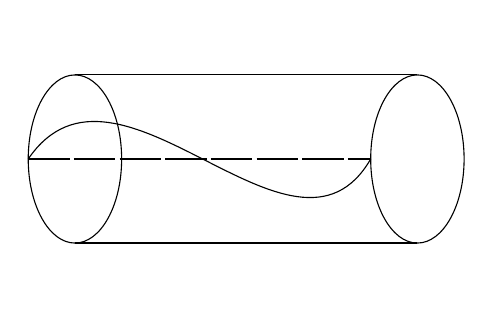
\begin{tikzpicture}[x=0.75pt,y=0.75pt,yscale=-1,xscale=1]
    %uncomment if require: \path (0,302); %set diagram left start at 0, and has height of 302

    %Shape: Ellipse [id:dp7113644287533367] 
    \draw   (220,160.5) .. controls (220,138.13) and (230.07,120) .. (242.5,120) .. controls (254.93,120) and (265,138.13) .. (265,160.5) .. controls (265,182.87) and (254.93,201) .. (242.5,201) .. controls (230.07,201) and (220,182.87) .. (220,160.5) -- cycle ;
    %Shape: Ellipse [id:dp2574876106229609] 
    \draw   (385,160.5) .. controls (385,138.13) and (395.07,120) .. (407.5,120) .. controls (419.93,120) and (430,138.13) .. (430,160.5) .. controls (430,182.87) and (419.93,201) .. (407.5,201) .. controls (395.07,201) and (385,182.87) .. (385,160.5) -- cycle ;
    %Straight Lines [id:da9747654267031158] 
    \draw    (242.5,120) -- (407.5,120) ;
    %Straight Lines [id:da6388065944921051] 
    \draw    (242.5,201) -- (407.5,201) ;
    %Straight Lines [id:da44727041223554886] 
    \draw  [dash pattern={on 15pt off 1.5pt}]  (220,160.5) -- (385,160.5) ;
    %Curve Lines [id:da44274218397801035] 
    \draw    (220,160.5) .. controls (263,97.5) and (348,224.5) .. (385,160.5) ;
  \end{tikzpicture}

\caption{A continuous section $s\colon [0,1]\to [0,1]\times \mathbb{R}/\mathbb{Z}$}
\end{figure}

\begin{definition}[{rotation number of closed interval}]
Fix a closed interval $[a,b]$ in $\mathbb{T}P^{1}$.
Let $s\colon [a,b]\to [a,b]\times \mathbb{R}/\mathbb{Z}$ be 
a continuous section of the canonical projection
$p\colon [a,b]\times \mathbb{R}/\mathbb{Z} \to [a,b]$
such that $s(a)=(a,0)$ and $s(b)=(b,0)$. 
The rotation number
is the homotopy class of the closed path
$q\circ s\colon [a,b]\to \mathbb{R}/\mathbb{Z}$
induced from $s$ and the canonical projection
$q\colon [a,b]\times \mathbb{R}/\mathbb{Z} 
\to \mathbb{R}/\mathbb{Z}$. Here, 
we identify $\pi_1(\mathbb{R}/\mathbb{Z},0)\simeq \mathbb{Z}$
via the canonical orientation of $\mathbb{R}/\mathbb{Z}$.
\end{definition}

\begin{proposition} \label{proposition-rotation-number}
Let 
$\phi \colon [a,b] \to [a,b]$ be an automorphism of 
a closed interval in $\mathbb{T}P^{1}$, 
$s\colon [a,b]\times \mathbb{R}/\mathbb{Z}$ and 
$\varphi \colon [a,b]\times \mathbb{R}/\mathbb{Z} \to 
[a,b]\times \mathbb{R}/\mathbb{Z}$ 
the symplectic automorphism induced from $\phi$.
Then, $\opn{rot}(\varphi\circ s)=\opn{rot}(s)$.
\end{proposition}
\begin{proof}
Since every automorphism of 
$[a,b]$ is a composition of the negation map 
with a translation map, we only need to consider the case
when $\phi$ is the negation map.
In this case, $\varphi(x,y)=(b+a-x,-y)$ for 
$(x,y)\in [a,b]\times \mathbb{R}/\mathbb{Z}$ if 
$a,b\notin \{-\infty,\infty\}$.
\end{proof}


From \cref{proposition-permissible-section} and \cref{proposition-rotation-number}, we can define the 
rotation number for every permissible smooth 
Cartier divisors as follows.
\begin{definition}[{cf. \cite{auroux2022lagrangian}}]
The \emph{rotation number} of $s$ is the sum of
the rotation number of all edges of $C$: 
\begin{align}
\opn{rot}(s)\deq \sum_{e\in \pi_0(C_0)}
\opn{rot}(s|_{\opn{cl}(e)}).
\end{align}

\end{definition}

\begin{definition}
Let $s\in \opn{CDiv}^{\infty}(C)$ be a smooth Cartier
divisor and $(U_i,f_i)_{i\in I}$ smooth Cartier data
of $s$. The data is \emph{good} if 
every $U_i$ is isomorphic to a contractible open 
neighborhood of $0$ in $\opn{LC}_{p}C$ where 
$p\in U_i$.
\end{definition}
If a smooth Cartier data $\{(U_i,f_i)\}_{i\in I}$ of $s$ 
is good,
we can calculate the divisor class $D_s$ of $s$ easily
by using \v{C}ech cohomology of sheaves:
\begin{align}
D_s=\{(f_j-f_i)\}_{i,j\in I}
\end{align}

\begin{proposition}
Let $s$ be an permissible smooth Cartier divisor on
a compact tropical curve $C$.
\label{equation-rotation-number}
\begin{align}
\opn{rot}(s)=\opn{deg}(D_s)(=\int_{C} c_1(D_s)).
\end{align}
\end{proposition}

\begin{proof}
Compare the \v{C}ech cocycle between smooth Cartier data and ordinary Cartier data.
\end{proof}

\begin{remark}
\label{remark-rotation-closed-interval} 
The above proposition 
is \emph{not} true for general compact metric curves.
Let $C\deq [0,1]$ be a closed interval
and $f_n\colon C\to \mathbb{R};x \mapsto nx^{2}$.
All $f_n$ is an permissible $(0,0)$-superform on $C$.
From the definition of smooth principal Cartier divisor,
$\opn{deg}(D_{(f_n)^{\mathrm{sm}}})=0$. 
A philosophical reason of this is that
a closed interval with finite length is a tropical
analog of a closed annulus in $\mathbb{C}$ but not for
a complex projective line (cf. 
\cite[Definition 3.7]{MR3903579}). In fact, $X(C_0)$ 
has a standard complex structure which is holomorphic to
an open annulus in $\mathbb{C}$.
\end{remark}

\begin{proposition}
\label{proposition-simple-interval-rr}
Let $C=[a,b]$ be a closed interval in $\mathbb{R}$
and $s$ an permissible smooth Cartier divisor 
such that $s_0\cap s=\{a,b\}$. Then,
\begin{align}
\chi(\opn{LMD}^{\bullet}(C;s))=\opn{rot}(s)+
\chi_{\opn{top}}(C).
\end{align}
\end{proposition}
\begin{proof}
We can calculate from 
\cref{proposition-n-valent} directly.
\end{proof}

A good point of the rotation number and the 
Euler number of $s$ is the 
following Meyer--Vietoris type lemma.

\begin{proposition}
\label{proposition-gluing-formula}
Let $s$ be an permissible smooth Cartier divisor on a
compact metric graph $C$ such that $s_0\cap s<\infty$.
Fix two closed metric subgraph of $C$ such that
$C' \cup C''=C$ and $C'\cap C''\subset s_0 \cap s$.
Then, 
the inclusion $i_{C'}\colon C'\to C$ 
and $i_{C''}\colon C''\to C$ induces
\begin{align}
\label{equation-meyer-vietoris}
\chi(\opn{LMD}^{\bullet}(C;s))
&=\chi(\opn{LMD}^{\bullet}(C';i_{C'}^{*}(s)))
+\chi(\opn{LMD}^{\bullet}(C'';i_{C''}^{*}(s)))
-\sharp(C'\cap C''), \\
\label{equation-rotation-sum}
\opn{rot}(s)&=\opn{rot}(i_{C'}^{*}(s))
+\opn{rot}(i_{C''}^{*}(s)).
\end{align}
\end{proposition}
\begin{proof}
From assumption $i^{*}_{C'}(s)$ and 
$i^{*}_{C''}(s)$ are permissible.
The \cref{equation-rotation-sum} is true from
the definition of rotation number. 
 Besides,
\begin{align}
s_0\cap i^{*}_{C'}(s)=i^{-1}_{C'}(s_0\cap s), \quad 
s_0\cap i^{*}_{C''}(s)=i^{-1}_{C''}(s_0\cap s), \quad
s_0\cap i^{*}_{C'\cap C''}(s)=
i^{-1}_{C'\cap C''}(s_0\cap s).
\end{align}
By \cref{proposition-n-valent} 
and Meyer--Vietoris sequence, we get 
the \cref{equation-meyer-vietoris}.
\end{proof}

We can generalize
\cref{proposition-simple-interval-rr} by
\cref{proposition-gluing-formula} as follows.

\begin{proposition}
\label{proposition-MRR-1-dim-poly-space}
Let $C$ be a compact pure $1$-dimensional rational 
polyhedral space satisfying \cref{condition-Rn} 
and $s$ a smooth Cartier divisor on $C$. Then,
\begin{align}
\chi(\opn{LMD}^{\bullet}(C;s))=\opn{rot}(s)+
\chi_{\opn{top}}(C).
\end{align}
\end{proposition}





\begin{proof}
Without loss of generality, we can assume $C$ is 
connected and $\sharp (s_0\cap s)\geq 1$.
Since $s_0\cap s\supset (C\setminus C_0)$, 
The set $s_0\cap s$ induces a cell decomposition of 
$C$. We will prove the theorem by mathematical 
induction for the cardinality of 
$\pi_0(C\setminus (s_0 \cap s))$, i.e., the 
number of edges of the cell decomposition.
When $\sharp\pi_0(C\setminus (s_0 \cap s))=1$, 
$C$ is homeomorphic to a closed interval 
or a closed circle and 
$\sharp (s_0\cap s)\leq 2$ 
from the definition of cell complex.
In this case, \cref{theorem-MRR-metric-graph} is 
true from \cref{proposition-n-valent} directly.

Suppose \cref{theorem-MRR-metric-graph} is true
for all smooth Cartier divisor $s$ on 
$C$ such that $\sharp \pi_0(C\setminus (s_0 \cap s))=n$.
Let $C$ be a $1$-dimensional 
compact rational polyhedral space
such that $\sharp\pi_0(C\setminus (s_0 \cap s))=n+1$.

Then, we can choose a pair of proper subgraph $C',C''$ of
$C$ such that
$C'\setminus (s_0\cap i^{*}_{C'}(s))\leq n$,
$C''\setminus (s_0\cap i^{*}_{C''}(s))\leq n$,
$C'\cup C''=C$
and $(C'\cap C'')\subset (s_0\cap s)$.

By \cref{proposition-gluing-formula}, we get 
\begin{align*}
\chi(\opn{LMD}^{\bullet}(C;s))
&=\chi(\opn{LMD}^{\bullet}(C';i_{C'}^{*}(s)))
+\chi(\opn{LMD}^{\bullet}(C'';i_{C''}^{*}(s)))
-\sharp(C'\cap C'') \\
&=\opn{rot}(i_{C'}^{*}(s))
+\opn{rot}(i_{C''}^{*}(s))
+\chi_{\opn{top}}(C')+\chi_{\opn{top}}(C'')
-\chi_{\opn{top}}(C'\cap C'') \\
&=\opn{rot}(s)+\chi_{\opn{top}}(C).
\end{align*}

\end{proof}

\begin{proof}[{Proof of \cref{theorem-MRR-metric-graph}}]
We can prove it from \cref{proposition-MRR-1-dim-poly-space}
and \cref{equation-rotation-number}.
\end{proof}


\subsection{MRR for general tropical curves}
\label{section-tropical-curve-general}
We will prove MRR for compact tropical curve 
without \cref{condition-Rn}. 
For general tropical curve $C$ with $1$-valent
vertex and smooth Cartier divisor 
$s\in\Gamma(C;\mathcal{A}^{0,0}_C/\mathcal{O}^{\times}_C)$,
we cannot choose a smooth Cartier divisor $s'$ which
is linearly equivalent to $s$ and $s_0\cap s'<\infty$.
The reason of this fact is that every 
$(0,0)$-superform on a compact tropical curve 
$C$ is constant on a sufficiently
small open neighborhood of $1$-valent vertex.
For instance, 
$f\colon \mathbb{T}^1 \to \mathbb{R}; x\mapsto 
\opn{log}(1+e^{x})$ is not a $(0,0)$-superform
on $\mathbb{T}^{1}$.
In this subsection, we extend smooth functions
on tropical curves for generalization of 
\cref{theorem-MRR-metric-graph} for general 
tropical curves.

\begin{definition} \label{definition-weak-smooth}
Let $\opn{exp}\colon \mathbb{T}^{n}\to 
\mathbb{R}_{\geq 0}^{n}$ be an exponential map of 
$\mathbb{T}^{n}$ and $U$ an open subset of 
$\mathbb{T}^{n}$.
A continuous function $f\colon U\to \mathbb{R}$
is a \emph{weak-smooth} if 
$f=\opn{log}\circ g\circ \opn{exp}$ for some 
smooth function $g\colon V\to \mathbb{R}_{>0}$ on 
an open subset $V$ of $\mathbb{R}^{n} 
(\supset \mathbb{R}_{\geq 0}^{n})$.
Let $\mathcal{A}_{\mathbb{T}^{n}}^{\mathrm{weak}}(U)$ 
be the set of weak-smooth functions on $U$.
\end{definition}
We can naturally generalize the sheaf of weak-smooth functions 
on rational polyhedral space by 
\cite[Lemma 9]{itenbergTropicalHomology2019b}.
\begin{example}
Let 
$g\in \mathbb{R}_{\geq 0}[x_1,\ldots,x_n]$ be a polynomial 
function with positive coefficients such that $g(0)\ne 0$. 
Then, $f=\opn{log}\circ g \circ \opn{exp}$ is weak-smooth 
on $\mathbb{T}^{n}$.
\end{example}

Since $\opn{log}\circ g\circ\opn{exp}+\opn{log}\circ h
\circ \opn{exp}=\opn{log}\circ(gh)\circ\opn{exp}$ and 
the condition is local, 
$\mathcal{A}_{\mathbb{T}^{n}}^{\opn{weak}}(U)$ forms a 
sheaf of Abelian groups on $\mathbb{T}^{n}$. 
The following property says that every weak-smooth 
function is sufficiently close to a constant function 
at the origin of $\mathbb{T}^{n}$.
\begin{proposition}
Let $U$ be an open neighborhood of the origin of 
$\mathbb{T}^{n}$ and 
 $f\in \mathcal{A}_{\mathbb{T}^{n}}^{\mathrm{weak}}(U)$.
For a given $\vep >0$, there exists $\delta\in \mathbb{R}$
such that $|\frac{\partial f}{\partial x_i}(z)|<\vep$
for any $z=(z_1,\ldots,z_n) \in (-\infty,\delta]^{n}$ and $i=1,\ldots,n$. 
Here, $\frac{\partial f}{\partial x_i}(z)$ is the $i$-th partial 
differential on $U\cap \mathbb{R}^{n}$.
\end{proposition}
\begin{proof}
For sufficiently small $\delta\in \mathbb{R}$, 
$[-\infty,\delta]^{n}$ is in $U$. 
We can assume $f=\opn{log}\circ g\circ \opn{exp}$ for
some smooth function 
$g\colon V\to \mathbb{R}_{>0}$ of $\mathbb{R}^{n} 
(\supset \mathbb{R}_{\geq 0}^{n})$.
By Jacobi rule, we have
\begin{align}
\frac{\partial f}{\partial x_i}(z)=(g\circ \opn{exp}(z))^{-1} 
\frac{\partial g}{\partial y_i}(\opn{exp}(z))\opn{exp}(z_i).
\end{align}
$g\circ \opn{exp}$ is bounded on $[-\infty,\delta]^{n}$.
$\frac{\partial g}{\partial y_i}$ can be defined 
on $V$, so $\frac{\partial g}{\partial y_i}\circ \opn{exp}$
is also bounded on $[-\infty,\delta]^{n}$.
Therefore, there exists a real number $r$ such that
$|(g\circ \opn{exp}(z))^{-1} 
\frac{\partial g}{\partial y_i}(\opn{exp}(z))|<r$ for any 
$x\in [-\infty,\delta]^{n}$.
Therefore, if $z_i$ is sufficiently small, so is 
$\frac{\partial f}{\partial x_i}(z_i)$. 
\end{proof}
From now on, we mainly discuss the case when $n=1$.

Let $C$ be a tropical curve. 
Let $\mathcal{A}_C^{\opn{weak}}$ be the sheaf 
of weak-smooth functions on $C$. From definition,
$\mathcal{A}_C^{0,0}\subset \mathcal{A}_C^{\opn{weak}}$
and $\mathcal{A}_C^{\opn{weak}}$ is also a fine sheaf.

We can replace $\mathcal{A}_C^{0,0}$ with 
$\mathcal{A}_C^{\opn{weak}}$
on \cref{equation-smoooth-cartier-divisor-sequence}
and thus we can also define smooth Cartier divisors
for weak-smooth functions. 
\begin{definition}
A \emph{weak-smooth Cartier divisor} of $C$ is a 
element of $\Gamma(C;\mathcal{A}_C^{\opn{weak}}/
\mathcal{O}^{\times}_C)$.
\end{definition}

Since $\mathcal{A}_C^{\opn{weak}}$ is fine, 
the connected homomorphism 
$\delta\colon \Gamma(C;\mathcal{A}_C^{\opn{weak}}/
\mathcal{O}^{\times}_C)\to \opn{Pic}(C)$ is 
surjective.


We can extend admissibility condition for
weak-smooth functions and weak-smooth Cartier 
divisors on $C$. In our case, every weak-smooth 
Cartier divisor satisfies the permissible condition 
at every $1$-valent vertex.
\begin{definition}
Let $s$ be an permissible weak-smooth Cartier divisor 
of $C$ such that $s_0\cap s<\infty$.
The Morse complex of $s$ the following graded module:
\begin{align}
  \opn{LMD}^{\bullet}(C;s)\deq \bigoplus_{p\in s_0\cap s} 
\tilde{H}^{\bullet-1}
(U_p\cap \{\tilde{f_p}<\tilde{f_p}(p)\};\mathbb{Z}).
\end{align}
Here, $(U_p,\tilde{f}_p)_{p\in s_0\cap s}$ is an
intersection data of $s$.
\end{definition}

From construction, the following theorem is just a
repetition of the proof of 
\cref{theorem-MRR-metric-graph}.

\begin{theorem} \label{theorem-MRR-tropical-curve}
Let $C$ be a compact tropical curve and 
$s$ an permissible weak-smooth Cartier divisor 
of $C$ such that $s_0\cap s<\infty$. Then,
\begin{align}
  \chi(\opn{LMD}^{\bullet}(C,s))=\opn{deg}(s)+
\chi_{\opn{top}}(C)=\opn{deg}(\mathcal{L})+1-g(C).
\end{align}
\end{theorem}


\begin{remark}
\label{remark-non-permissible-divisor}
We explain the reason why we add permissible condition for 
smooth Cartier divisors. 
One of reasons is that there exists smooth function $f$
on a polyhedral space $S$ and 
$x\notin\opn{Crit}(f|_S)$ such that
$\opn{LMD}^{\bullet}(A_S,f|_{S},x)$ is nontrivial.
Another reason is that we could not create 
convenient continuous sections like 
\cref{definition-continuous-section} easily.

The third reason is the most critical. 
We will explain about this problem by the following 
example:
Let 
$g$ be a weak-smooth function on 
$\Gamma_3$
such that 
\begin{enumerate}
\item $dg=(\frac{1}{2},\frac{1}{2})$,
\item $\opn{Crit}(g)=\Gamma_3\setminus \Gamma_3^{\circ}$,
\item $\sum_{p\in \opn{Crit}(g)}\opn{ind}_p(g)=2$.
\end{enumerate}
$g$ is permissible except $x=(0,0)$.
If we generalize 
\cref{theorem-MRR-tropical-curve} for $g$, 
we need to add the index $\opn{ind}_x(g)$ at $x$ satisfying
\begin{align}
\sum_{p\in \opn{Crit}(g)}\opn{ind}_p(g)+
\opn{ind}_x(g)=1=\chi_{\opn{top}}(\Gamma_3).
\end{align}
At least, \cref{theorem-MRR-tropical-curve} is not
true without correction the effect at non-permissible point
of $g$.
In this case, $\opn{ind}_x(g)$ should be $-1$.
This condition is independent of the choice
of $g$ satisfying the above condition.
On the other hand, the index of smooth Cartier
divisor should be independent of the choice of
Cartier data.
Since $\opn{ind}_x(g+m)$ depends on the choice
of monomials $m$, we need to choose a monomial $m_0$
with integer slope to 
define the index of $g$ at $x$ as a divisor.
We consider there is no canonical choice
of $m_0$ for $g$ as a principal divisor without
assumption admissibility.
Every permissible function $f$ has a canonical choice
of monomials which is determined by the condition 
whether $x\in \opn{Crit}(f+m)$ or not.
We could not use this condition for $g$ since 
$x\notin \opn{Crit}(g+m)$ for every monomial with
integer slope.
\end{remark}

\begin{remark}
Our definition of smooth Cartier divisor 
has an analog of positive divisor by using 
the local data $\{(U_i,f_i)\}_{i\in I}$ as 
explained in \cref{example-tropical-kodaira-vanishing}.
However, this positive divisor is different 
from ample line bundles for tropical curves. 
If $s$ is a positive smooth Cartier divisor, then
$\chi(\opn{LMD}(C;s))=\sharp(s_0\cap s)\geq \sharp 
(C\setminus C_{\opn{reg}})$. 
Thus, $\chi(\opn{LMD}(C;s))\geq 2g(C)-2$
when $C$ is a compact trivalent
graph with no $1$-valent vertex. This means that
$\opn{deg}(s)\geq 3g(C)-3$.
On the other hand, every divisor $D$ satisfying
$\opn{deg}(D)>0$ is ample \cite[Corollary 43]{MR2892941}.
In other words, there is no direct tropical
analog of Kodaira embedding theorem
in tropical geometry.
\end{remark}



\subsection{Relationships between previous results}
\label{section-tropical-curve-note}


\subsubsection{Relationships between
homological mirror symmetry of trivalent graphs}
\label{section-syz-trivalent-graph}

Our approach is mostly affected from 
\cite{auroux2022lagrangian}.

\begin{remark} \label{rmk: curve_mirror}
When $C$ is a trivalent metric graph, 
our Lagrangian sections are 
almost the same with that of fiberwise wrapped Fukaya category 
$\mcal{F}(M)$ \cite[3.1]{auroux2022lagrangian}.
Here, $M$ is the
union of $\C P^{1}$'s whose intersection complex is $C$, 
i.e., every edge of $C$ corresponds
$\C P^{1}$ and every trivalent vertex of $C$ corresponds
to the intersection points of some three $\C P^{1}$'s.
The mirror manifold of $M$ is an algebraic curve $X_K$
from Mumford's construction using the dual intersection
complex $C$.

The local model of $M$ comes from the critical locus
of the potential function of a (A-side) Landau--Ginzburg 
model $(\C^{3},-xyz)$. There exists a (Orlov) functor
from $\opn{Fuk}(\C^{3},-xyz)$ 
to $\opn{wFuk}((\C^{\times})^2)$ which is compatible
with the pushforward 
$i_*\colon \opn{Perf}(V(1+x_1+x_2))\to \opn{Perf}((K^{\times})^{2})$. 
of the inclusion $i\colon V(1+x_1+x_2)\hookto (K^{\times})^2$
via mirror functors (see \cite[2.]{auroux2022lagrangian}
for more details). 

The mirror space $M$ of $X_K$ can be considered as a 
topological compactification of $\check{X}_0(C)$.
By a slight modification of $\check{X}_0(C)$, every 
stratified smooth Lagrangian section of $\check{X}(C)$ 
can be considered as an object of $\mcal{F}(M)$.

The main difference between our setting and 
that of \cite{auroux2022lagrangian} 
is the definition of graded space $\opn{LMD}(C,s)$. 
Our approach haven't got no good definition 
of $m^{d}$-operations yet, 
but we can define $\opn{LMD}(C,s)$ 
without Hamiltonian
perturbations.
\end{remark}

The stratified torus fibration of Riemann surface is 
closely related with pants decomposition, and thus
Auroux--Efimov--Katzarkov in \cite{auroux2022lagrangian} 
expect a homological mirror symmetry 
for projective hypersurfaces since they have higher 
dimensional pants decomposition \cite{MR2079993} along
tropical hypersurfaces.




\begin{definition}[{cf. \cite{auroux2022lagrangian}}]
An permissible smooth Cartier divisor $s$ is 
\emph{simple} if there exists a local intersection data
$\{(U_p,f_p)\}_{p\in s_0\cap s}$ such that
$f_p$ is strictly convex at all $p\in C\setminus C_0$.
\end{definition}

\subsubsection{Relationships between 
Poincar\'e--Hopf theorem for graphs}

\cref{theorem-MRR-metric-graph} can be considered 
as a certain variation of Knill's graph 
theoretical Poincar\'e--Hopf theorem \cite{knill2012graph}
or 
Banchoff's critical point theorem \cite{MR225327}.
We can easily see the index $i(v)$ defined in 
\cite[\textsection 3]{knill2012graph}
corresponds to $\opn{ind}_v(f)$ defined in 
\cref{equation-local-index} (see also 
\cref{proposition-n-valent} and 
\cite[\textsection 7]{knill2012graph}).

Banchoff proved a polyhedral complex version of Poincar\'e--Hopf theorem
for height functions \cite[Theorem 1]{MR225327}.
The definition of the index $a(v,f)$ 
\cite[p.246]{MR225327} which 
he used for the theorem may seem different 
from our index but essentially equal to it
(see also \cite[p.143-144]{grunert2017piecewise} 
for more detail about it).





\subsubsection{Relationships with a localization of 
index on compact Riemann surfaces.}

We mention the relationship between 
\cref{theorem-MRR-tropical-curve} and
\cite[6]{MR2676658}.
For simplicity,
we assume $C$ is a compact trivalent tropical curve, i.e.,
a compact tropical curve which only has $3$-valent
vertex in $C\setminus C_0$.  
$C_0$ has a canonical dual torus fibration 
$\pi_{C_0}\colon X(C_0)\to C_0$ of
$\check{\pi}_{C_0} \colon \check{X}(C_0)\to C_0$.
We can define $X_0(C)\deq C\sqcup_{i,s} X(C_0)$ like
$\check{X}_0(C)$.
$C$ has a canonical lattice length metric $d_{C}$, and
thus we can define the following set for sufficiently small
$\vep >0$: 
\begin{align}
C_{0,\vep}\deq \{p\in C\mid d_C(p,v)>\vep 
\text{ for all } v\in C\setminus C_0\}.
\end{align}

For a given $\vep>0$ (and a \emph{signed tropical structure}
on $C$ \cite{MR3076066}), 
$X_0(C)$ can be considered as a subset of a compact 
Riemann surface $X$ whose complex structure is 
compatible with $X(C_{0,\vep})$. 
Such a $X$ is given by gluing triangles for 
each open neighborhood of $p\in X_0(C)\setminus X(C_0)$
appropriately.
Let $s$ be an permissible smooth Cartier divisor on $C$.
$s|_{C_0}$ corresponds to a Lagrangian section of 
$\check{\pi}_{C_0}$ from 
\cref{proposition-cartier-lagrangian}.
By SYZ transformation,
\myfootnote{By philosophy of SYZ mirror symmetry,
we should consider Lagrangian section 
as a mirror of complex line bundle,
and we also explain about it for tropical tori in 
\cref{example-SYZ-trasform-tori}.
}
$s|_ {C_0}$ induces a family of $U(1)$-holonomoy for
each torus fiber $\pi_{C_0}^{-1}(p)$ and defines a 
complex line bundle on $C_{0,\vep}$. From now on, 
we suppose $s_0\cap s<\infty$. 
Let $\{(U_p, f_p)\}_{p\in s_0\cap s}$ be the local intersection data 
of $s$ such that 
$\{x\in C\mid d_C(p,x)\leq \vep\}\subset U_p$ for
all $p\in C\setminus C_0$.

Besides, we suppose 
$(s\cap s_0)\setminus C_{0,\vep}=C\setminus C_0$ and $s$ satisfies the following cocycle
condition for each $p\in C\setminus C_0$:
\begin{align}
df_p(p_1)+df_p(p_2)+df_p(p_3)=0,\quad 
(\{p_1,p_2,p_3\}\deq \{x\in C\mid d_C(p,x)=\vep\}).
\end{align}

From the above condition, $0<|df_p(p_i)| \ll 1$ and
$f$ is of type $s_{2,1}$ or $s_{1,2}$ discussed
in \cref{proposition-n-valent}.
From the above condition, we can define 
a flat $U(1)$-bundle on each pants of a 
connected component of $X\setminus X(C_{0,\vep})$
as like \cite[6.1.3]{MR2676658}.
We remark the isomorphism
$(\mathcal{F}_{\mathbb{Z},C}^{1})_p\otimes_{\mathbb{Z}}
\mathbb{R}/\mathbb{Z}\simeq 
H^1(\mathbb{P}^{1}\setminus 
\{0,1,\infty\};\mathbb{R}/\mathbb{Z})$
is important for this construction.
The $s_{2,1}$
corresponds a small pants and the $s_{1,2}$
corresponds a large pants in 
\cite[Definition 6.3]{MR2676658}.


Each small pants and large pants have a local 
Riemann--Roch number defined the theory of 
localization of Dirac-type operator and its 
number is equal 
to our index by the above correspondence.
\myfootnote{
We also thanks Jin Miyazawa
for explaining us a heart of localization of 
the index of Dirac operator and answering some 
questions about it.}

The following equation is a correspondence about 
local index $\opn{ind}_v$ and the Local 
Riemann--Roch number under the above 
identification \cite[Theorem 6.7]{MR2676658}.
\begin{align} \label{equation-local-RR}
& [BS^{+}]=\opn{ind}_v(s_{2,0})=1, 
&& [BS^{-}]=\opn{ind}_v(s_{0,2})=-1,\notag \\
& [D^{+}]=\opn{ind}_v(s_{1,0})=1,
&& [D^{-}]=\opn{ind}_v(s_{0,1})=0, \\
& [P^{S}]=\opn{ind}_v(s_{2,1})=0,
&& [P^{L}]=\opn{ind}_v(s_{1,2})=-1 \notag.
\end{align}
The origin of our approach firstly comes from the 
above correspondence.
\myfootnote{
We also thank Yoshinori Gongyo for 
giving a question about relationships 
between a kind of Pick's formula for
tropical Kummer surfaces and Atiyah--Singer
index formula. This question gives me 
an opportunity to learn geometric prequantization and
Bohr--Sommerfeld points.
}
From this correspondence, 
our theorem for tropical curve can be 
proved by the theory of localization of index 
and classical Riemann--Roch formula.
We stress that both method of computation
of our index and the local Riemann--Roch number
defined in \cite{MR2676658} are different 
each other even though both indexes have various 
similar features.
We also note that it was the beginning of our 
approach that we 
noticed the above correspondence.
We can also consider the following question as 
like \cite{auroux2022lagrangian}.

\begin{question} \label{question-tropical-complex-rr}
Can we generalize the 
above correspondence \ref{equation-local-RR}
for more general the complement of
projective hyperplane arrangements and flat $U(1)$-bundles on it?
How about for pants decomposition of
  complex algebraic hypersurfaces in \cite{MR2079993} and line bundles?
\end{question}

We add two comments about the above question. 
First, the Bergman fan $\Sigma$ of a given complex 
(projective) hyperplane arrangement $\mathcal{A}$ does \emph{not} 
determine 
the homotopy type of the complement of (projective) 
hyperplane
arrangements $U(\mathcal{A})$ uniquely in general.
Second, every flat $U(1)$-bundle on 
$U(\mathcal{A})$ is, 
however, given
from a group homomorphism 
$\rho\colon T_{|\Sigma|,0}^{\mathbb{Z}}\to 
\mathbb{R}/\mathbb{Z}$ since 
$T_{|\Sigma|,0}^{\mathbb{Z}}\simeq 
H_1(U(\mathcal{A});\mathbb{Z})$ (see \cite[Theorem 4]{MR3153919}).
Therefore, we hope that we can get an affirmative answer 
for \cref{question-tropical-complex-rr}.

\section{Proof for integral affine manifold with Hessian form.}
\label{section-integral-affine-manifold}
In this section,
we recall the notion of affine manifolds from
\cite{MR2293045,
goldmanRadianceObstructionParallel1984a,
MR2181810,
grossMirrorSymmetryLogarithmic2006a} and 
\cite[Chapter 6]{MR2567952}.

\begin{definition} \label{definition-integral-affine-manifold}
An $n$-dimensional \emph{integral affine 
(resp. strongly integral affine, affine)} manifold
is a pair of an $n$-dimensional differential manifold $B_0$ 
and an atlas $\{(U_i,\psi_i)\}_{i \in I}$ of $B_0$ such that 
$\psi_i \circ \psi_j^{-1}$ is a restriction of 
an element in $\opn{GL}_n(\mathbb{Z})\ltimes \mathbb{R}^{n}$
(resp. $\opn{GL}_n(\mathbb{Z})\ltimes \mathbb{Z}^{n}$,
$\opn{GL}_n(\mathbb{R})\ltimes \mathbb{R}^{n}$) for any $i,j\in I$.
\end{definition}

\begin{remark}
An (integral) affine manifold is a special case of 
$(G,X)$-manifolds \cite[3.3]{MR1435975}.

The terminology integral affine manifold has 
different terminologies for different authors. 

For instance, an integral (resp. strongly integral) affine manifold 
is called a tropical affine manifold (resp. integral affine manifold)
in \cite[Definition 1.22]{MR2722115}. 
The terminology `strongly integral affine manifold' 
comes from \cite[Remark 5.10]{MR3079343}.
\end{remark}


We can consider a sheaf theoretic definition of 
integral affine manifold as explained 
in \cite[2.1]{MR2181810} 
and every integral affine manifold is a special case of 
tropical manifold. 
Every integral affine structure of $B_0$ induces a 
canonical local system $\mathcal{T}_{\mathbb{Z},B_0}$ 
of integer valued vector bundle and the dual 
local system $\mathcal{T}_{\mathbb{Z},B_0}^{\vee}$ of it.



Let $(B_0,\{(U_i,\psi_i)\}_{i \in I})$ be an affine manifold.
Every  $U_i$ has a coordinate system $\{x_k\}_{k=1,\ldots,n}$ 
induced from a coordinate system formed 
by affine functions on $\mathbb{R}^{n}$.
We call this coordinate system \emph{affine coordinate system} 
of $U_i$. 

\begin{definition}
A \emph{Hessian metric} or \emph{metric of Hessian form} on an affine manifold 
$(B,\{(U_i,\psi_i)\}_{i \in I})$.
is a Riemannian metric $g$ such that 
there exists a multi-valued function $K$ on $B$ satisfying
$g=\sum_{k,l}\frac{\partial K}{\partial x_k \partial x_l}dx_k dx_l$ for 
an affine conndinate system of $U_i$. The triple
$(B,\{(U_i,\psi_i)\}_{i \in I},g)$ is called a \emph{Hessian manifold}.
\end{definition}
\begin{remark}
We follows the terminology Hessian metric and Hessian manifold 
from \cite{MR2293045}.
The terminology 
Hessian manifold is called
\ind{K\"ahler affine manifold}{Kahler affine manifold}
in \cite{MR714338}, \ind{affine K\"ahler manifold}{affine Kahler manifold}
or AK-manifold for short.
In the respect of historical order, we should use the latter name.
However, we usually use the former name for avoiding confusion
with K\"ahler manifold with affine structure.
\end{remark}


\begin{example}
Let $f \colon \mathbb{R}^{n} \to \mathbb{R}$ be a continuous function defined by 
\cref{equation-log-polynomial}.
$f$ is smooth and convex 
on $\mathbb{R}^{n}$.
Therefore, $(\mathbb{R}^{n},f)$ form an integral 
Hessian manifold. This is a typical example of
Hessian domain.
See also \cite[Appendix 2]{MR1301331} for general theory for
the relationships for Hessian form and 
the induced K\"{a}hler potential on
toric manifolds.
\end{example}

A Hessian metric can be considered as a $(1,1)$-superform 
naturally and this superform is a certain analog of 
K\"ahler form, so Hessian metric itself is called Hessian form.

\begin{remark} \label{remark-compact-hessian}
By \cite[Theorem 2.1 and Corollary 2.3]{MR714338},
every closed special Hessian manifold $(B_0,g)$ has 
a flat Riemannian and Hessian metric $\tilde{g}$ such 
that its volume form $\opn{vol}_{\tilde{g}}$ is parallel 
with respect to the
affine connection induced from the affine structure 
on $B_0$.
Therefore, the associated first and second Koszul 
form of $\opn{vol}_{\tilde{g}}$ is trivial 
\cite[Definition 3.1.2]{MR2293045}.
By \cite[Theorem 8.3.3]{MR2293045}
the Levi--Civita connection of $\tilde{g}$ is 
equal to the affine connection of $B_0$ 
\cite[Corollary 8.3.7]{MR2293045}. 
By Bieberbach theorem, every closed flat Riemannian manifold 
is covered by a Riemannian flat torus and thus every closed 
integral Hessian manifold is an unramified cover of 
a tropical torus as mentioned in \cite[5.2]{MR1882331}.
\end{remark}

\begin{remark}
The integral affine structure itself is a very strict condition.
\ind{Chern's conjecture}{Chern's conjecture} states 
every closed affine manifold $B_0$ has zero topological 
Euler characteristic.
If $B_0$ is a closed flat Riemannian manifold, Chern's conjecture is true from Chern--Gauss--Bonnet formula.
This conjecture is true for 
\emph{special affine manifold} \cite{MR3665000},
i.e., an affine manifold $(B, \{U_i,\psi_i\}_{i\in I})$ 
whose transition map is 
in $\opn{SL}_n(\mathbb{R})\ltimes \mathbb{R}^{n}$.
Therefore, every closed integral affine manifold satisfies Chern's conjecture since the orientable double over of an integral affine manifold has a compatible special integral affine structure.
\myfootnote{We have not checked 
the original source of Chern's conjecture yet.
Our knowledge about these conjectures
mainly comes from \cite{goldmanRadianceObstructionParallel1984a}
and \cite{MR3665000}.
}
\end{remark}

\begin{remark}[{Relationships between symplectic geometry}]
Integral affine manifolds naturally appear 
as base spaces of Lagrangian torus fibration 
\cite{duistermaatGlobalActionangleCoordinates1980a}. 
Besides, the deformation space of 
special Lagrangian submanifolds of
a Calabi-Yau $n$-fold with a nowhere vanishing 
holomorphic $n$-form has 
an integral affine structure with 
a Hessian metric by McLean's theorem \cite{MR1664890}.
See also \cref{appendix-geometric-quantization} 
for the relationships between integral affine manifolds 
and geometric quantization. 
\end{remark}







\subsection{Tropical homology, Tropical superform and Cartier data}
From now on, we follow about tropical homology and sheaf 
theory for tropical manifolds
from \cite{mikhalkinTropicalEigenwaveIntermediate2014a,
MR3903579,gross2019sheaftheoretic}.
In the case of affine manifold, this sheaf is already
studied in the field of Hessian geometry as a vector bundle
with a flat connection
(e.g. \cite[Chapter 7]{MR2293045}).
Let $\mathcal{F}^{p}_{\mathbb{Z},X}$ be 
the sheaf defined in 
\cite[2.4]{mikhalkinTropicalEigenwaveIntermediate2014a}
where $p\in \mathbb{Z}_{\geq 0}$.
 (We follow the notation in \cite[Definition 2.4]{MR3894860}.)
If $X$ is a tropical manifold, then 
$\mathcal{F}^{p}_{\mathbb{Z},X}$ is equal 
to the sheaf $\Omega_{X}^{p}$ of tropical $p$-forms 
\cite[Definition 2.7]{gross2019sheaftheoretic}
(see \cite[Remark 2.8]{gross2019sheaftheoretic}).
Throughout in this paper, we assume every rational polyhedral space $X$
satisfies $\Omega_X^{p}\simeq \mathcal{F}_{\mathbb{Z},X}^{p}$
for all $p$.
Let $\mathcal{W}_{p,X}^{\mathbb{Z}}
\deq \mathcal{H}om(\mathcal{F}^{p}_{\mathbb{Z},X},\mathbb{Z}_X)$
be the sheaf of $p$-th wave tangent spaces 
\cite{yamamotoTropicalContractionsIntegral2021,mikhalkinTropicalEigenwaveIntermediate2014a}.
We set $\mathcal{F}^{p}_{X}\deq 
\mathcal{F}^{p}_{\mathbb{Z}, X}
\otimes_{\mathbb{Z}_X}\mathbb{R}_X$ and 
$\mathcal{W}_{p,X}\deq 
\mathcal{W}_{p,X}^{\mathbb{Z}}
\otimes_{\mathbb{Z}_X}\mathbb{R}_X$.



\begin{example}
If $B_0$ is an integral affine manifold, then 
$\mathcal{F}^{p}_{\mathbb{Z},B_0}\simeq 
\bigwedge^{p}_{i=1} \mathcal{T}_{\mathbb{Z},B_0}^{\vee}$ for 
all $p\in \mathbb{Z}_{\geq 0}$ and
$\mathcal{W}^{\mathbb{Z}}_{p,B_0}\simeq 
\bigwedge_{i=1}^{p}\mathcal{T}_{\mathbb{Z},B_0}$.
\end{example}

 

We recall some results about tropical superforms from
\cite{MR3903579,smacka2017differential}.
Let $\mathcal{A}^{p,q}_X$ be the sheaf of 
$(p,q)$-superforms on $X$. 
\begin{example}
$\mathcal{A}_X^{0,0}$ can be considered as the 
sheaf of smooth functions on $X$.
In fact, $\mathcal{A}_X^{0,0}$ is isomorphic to 
the sheaf $\mathcal{C}^{\infty}(X)$ of smooth functions 
on $X$ if $X$ is an integral affine manifold.
\end{example}
The bigraded sheaf $\mathcal{A}_X^{\bullet,*}$ has 
a canonical bigraded
complex structure
$(\mathcal{A}_X^{\bullet,*},d',d'')$.

$\mcal{F}^{p}_{X}$ has the following acyclic resolution
\cite[Corollary 3.18, Lemma 3.21]{MR3903579}:
\begin{align}
  0 \to \mcal{F}^{p}_{X} \to \mcal{A}^{p,0}_{X}\xto{d''} 
\mcal{A}^{p,1}_{X} \xto{d''}\cdots.
\end{align}

$(\mathcal{F}_{\mathbb{Z},X}^{\bullet},d')$ has a canonical dga structure, 
and thus its hypercohomology 
$\mb{H}^{\bullet}(X;\mcal{F}_{\mathbb{Z},X}^{\bullet})$ is a 
graded-commutative algebra. 
This is a certain tropical analog of the singular cohomology
$H^{\bullet}(X;\C)$ for a complex manifold $X$ since 
the analytic de Rham theorem $\C_X \simeq \Omega_X^{\bullet}$ 
gives isomorphism 
$H^{\bullet}(X;\C)\simeq \mb{H}^{\bullet}(X;\Omega_X^{\bullet})$
of graded algebras. 

An elementary but remarkable fact of 
$(\mcal{F}_{\mathbb{Z},X}^{\bullet},d')$ is that 
$\mcal{F}_{\mathbb{Z},X}^{\bullet}\simeq 
\bigoplus_{i\in \Z}\mcal{F}_{\mathbb{Z},X}^{i}[-i]$, i.e., the differential 
of $\mcal{F}_{B}^{\bullet}$ is trivial unlike the analytic de Rham complex
of complex manifolds, see \cite[Corollary 2.15]{smacka2017differential}.
Therefore, we can calculate the multiplication of 
$\mb{H}^{\bullet}(X;\mcal{F}_{\mathbb{Z},X}^{\bullet})$ by 
cup product of each $H^{q}(X;\mcal{F}_{\mathbb{Z},X}^{p})$ easily.

Let $f\colon X\to Y$ be a morphism of rational polyhedral 
space. Then, this induces a canonical morphism
\begin{align}
b_f^{p}\colon \mathcal{F}^{p}_{\mathbb{Z},Y}\to 
f_* \mathcal{F}^{p}_{\mathbb{Z},X} \to
Rf_*\mathcal{F}^{p}_{\mathbb{Z},X}
\end{align}
for all $p\in \mathbb{Z}_{\geq 0}$ and the pullback 
$f^{*}\colon 
\mb{H}^{\bullet}(Y;\mcal{F}_{\Z, Y}^{\bullet})\to 
\mb{H}^{\bullet}(X;\mcal{F}_{\Z, X}^{\bullet})$
\cite[Proposition 4.17]{gross2019sheaftheoretic}.
The pullback $f^{*}$ is a graded ring homomorphism. 

The canonical monomorphism $\mcal{O}^{\times}_X \to \mcal{A}^{0,0}_X$
induces the following commutative diagram 
\myfootnote{Several similar diagrams for some special tropical spaces 
and similar spaces appear
in literature, e.g. \cite[p.468]{MR2567952}
and \cite[Definition 1.45]{grossMirrorSymmetryLogarithmic2006a}.}:

\begin{equation} \label{equation-smooth-cartier-diagram}
  \begin{tikzcd}
    & 0 \arrow[d]    & 0 \arrow[d]           &                      &   \\
    & \mb{R}_{X} \arrow[r,equal] \arrow[d]   & \mb{R}_{X} \arrow[d]\\
0\arrow[r] & \mathcal{O}_X^{\times} \arrow[r] \arrow[d] &
\mcal{A}^{0,0}_X \arrow[r] \arrow[d] & \mcal{A}^{0,0}_X /\mcal{O}_{X}^{\times}  \arrow[r] \arrow[d,equal] & 0 \\
    0 \arrow[r] & 
\mathcal{F}_{\mathbb{Z},X}^{1} \arrow[r] \arrow[d] & 
\mcal{Z}^{1}_{X} \arrow[r] \arrow[d]  & \mcal{Z}^{1}_{X}/
\mathcal{F}_{\mathbb{Z},X}^{1} \arrow[r]   & 0 \\
    & 0 & 0 &  &
  \end{tikzcd}
\end{equation}
Here $\mcal{Z}^{q}_{X}\deq
  \opn{Ker}(d'': \mcal{A}^{0,q}_X\to \mcal{A}^{0,q+1}_X)$.
Every row and column of the diagram (\ref{equation-smooth-cartier-diagram}) is exact
and $\mcal{A}_{X}^{0,0}/\mcal{O}^{\times}_X
  \simeq \mcal{Z}^{1}_X/\mcal{F}_{\Z,X}^{1}$ from the snake lemma.
The left column short exact sequence of 
\cref{equation-smooth-cartier-diagram} is called
the 
\ind{tropical exponential sequence}{tropicalexponentialexactsequence}
(e.g. \cite{MR3894860}).

By taking the long exact sequence for 
\cref{equation-smooth-cartier-diagram}, we get a canonical morphism:
\begin{align} \label{equation-tropical-cartier}
c_1\colon \opn{CaDiv}^{\infty}(X)\to \opn{Pic}(X)\to 
H^{1}(X;\mathcal{F}_{\mathbb{Z},X}^{1}); s\mapsto D_s 
\mapsto c_1(D_s).
\end{align}
The second morphism of (\ref{equation-tropical-cartier}) is 
called the Chern class map of 
$\opn{Pic}(X)$ in \cite[5]{mikhalkinTropicalCurvesTheir2008a}.
Let $f\colon X\to Y$ be a morphism of 
two rational polyhedral spaces.
From definition of morphism of rational polyhedral space
and a naturally induced morphism of superforms 
\cite[Lemma 2.21]{MR3903579},
$f$ induces the pullback 
$f^{*}\colon \opn{CaDiv}^{\infty}(Y)\to \opn{CaDiv}^{\infty}(X)$ 
and $c_1(f^{*}s)=f^{*}(c_1(s))$ from the diagram
(\ref{equation-smooth-cartier-diagram}). 
In particular, we have
$c_1(f^{*}(s)^{n})=f^{*}(c_1(s)^{n})$ for every 
$D\in\opn{CaDiv}^{\infty}(Y)$
by \cite[Proposition 4.17]{gross2019sheaftheoretic}.

\subsection{Verdier duality and Borel--Moore homology
for tropical spaces}
In this subsection, we recall Verdier duality for
tropical manifolds.
See \cref{section-verdier-dual} if you do not familiar 
with Verdier duality.
Every rational polyhedral space $X$ is locally compact, 
and thus we can use Verdier duality of tropical spaces.
We set $H^{p,q}(X;\mathbb{Z})\deq 
H^{q}(X;\mathcal{F}_{\mathbb{Z},X}^{p})$. 
Let $\upomega_X^{\bullet}$ be the dualizing complex 
of $D^{b}(\mathbb{Z}_X)$.
The $(p,q)$-th Borel--Moore homology of $X$ is
\begin{align}
H^{\opn{BM}}_{p,q}(X;\Z)\deq 
H^{-q}R\opn{Hom}(\mathcal{F}_{\mathbb{Z},X}^{p},\upomega_X^{\bullet})\simeq 
\opn{Hom}_{D^{b}(\mathbb{Z}_X)}(\mathcal{F}_{\mathbb{Z},X}^{p}[q],\upomega_X^{\bullet}).
\end{align}
$H_{0,q}^{\opn{BM}}(X;\Z)=
H^{-q}R\opn{Hom}(A_X,\upomega_X^{\bullet})$ 
is equal to the classical $p$-th Borel--Moore homology
\cite[Lemma 4.8]{gross2019sheaftheoretic}.
We note $H_{0,0}^{\opn{BM}}(X;\mathbb{Z})\simeq 
 \mathbb{Z}$ if 
$X$ is compact and path-connected.
The isomorphism follows from the universal 
coefficient theorem and 
$H^{1}_c(X;\mathbb{Z})$ is finitely generated and
torsion-free 
\cite[VI.Proposition 5.3]{iversenCohomologySheaves1986a}.

Let $f$ be a proper morphism of rational polyhedral 
spaces.
Then, there exists the pushforward
$f_*\colon H_{p,q}^{\mathrm{BM}}(X;\mathbb{Z})
\to H_{p,q}^{\mathrm{BM}}(Y;\mathbb{Z})$
of tropical Borel--Moore homology 
\cite[Definition 4.9]{gross2019sheaftheoretic}:
\begin{align}
f_*(\psi)\deq \opn{Tr}_{f,\upomega_Y^{\bullet}}\circ 
Rf_!\psi \circ b_{f}^{p}[q]\in 
\opn{Hom}_{D^{b}(\mathbb{Z}_X)}(
\mathcal{F}^{p}_{\mathbb{Z},Y}[q],\upomega_Y^{\bullet}).
\end{align}

\begin{example}

If $p=0$, $q=0$ and $f=a_X$, 
then $b^{0}_{a_X}$ is just a counit for 
the adjoint $a^{-1}_X\dashv Ra_{X*}$.
Therefore, we can identify
$a_{X*}\colon H_{\opn{BM}}^{0,0}(X;\mathbb{Z})
\to H_{\opn{BM}}^{0,0}(\{\opn{pt}\};\mathbb{Z})$
with $\opn{Hom}_{D(\mathbb{Z})}(\mathbb{Z},\opn{Tr}_{a_X,\mathbb{Z}})$
by the adjoint isomorphism
$\opn{Hom}_{D(\mathbb{Z}_X)}(a_X^{-1}\mathbb{Z},
\upomega_X^{\bullet})\simeq 
\opn{Hom}_{D(\mathbb{Z})}(\mathbb{Z},Ra_{X*}\upomega_X^{\bullet})$
if $a_X$ is proper.

\end{example}

Let $f\colon X\to Y$, $g\colon Y\to Z$ be a proper 
morphism of rational polyhedral spaces.
Then, $f_*\circ g_*=(f\circ g)_*$ from 
\cref{equation-trace}.

Tropical cohomology and tropical Borel--Moore homology 
also have cap product 
\cite[\textsection 4.6]{gross2019sheaftheoretic}:
\begin{align}
\cdot \frown \cdot \colon
H^{i,j}(X;\mathbb{Z}) \times 
H_{p,q}^{\mathrm{BM}}(X;\mathbb{Z})\to 
H_{p-i,q-j}^{\mathrm{BM}}(X;\mathbb{Z});(c,\alpha) 
\mapsto c\frown \alpha.
\end{align}

If $p=i$ and $q=j$, then the cap product $c\frown \alpha$ 
is just the composition $\alpha \circ c$ of 
morphisms:
\begin{align} \label{equation-composition-cap}
\cdot \frown \cdot =\cdot \circ \cdot \colon
\opn{Hom}_{D^{b}(\mathbb{Z}_X)}(
\mathbb{Z}_X,\mathcal{F}^{p}_{\mathbb{Z},X}[q])\times
\opn{Hom}_{D^{b}(\mathbb{Z}_X)}
(\mathcal{F}^{p}_{\mathbb{Z},X}[q],\upomega_X^{\bullet})
\to 
\opn{Hom}_{D^{b}(\mathbb{Z}_X)}(\mathbb{Z}_X,
\upomega_X^{\bullet}).
\end{align}

Let $f\colon X \to Y $ be a proper morphism of 
rational polyhedral spaces.
Then, there exists the projective formula 
for $\alpha\in H_{p,q}^{\mathrm{BM}}(X)$
and $c\in H^{i,j}(Y)$ 
\cite[Proposition 4.18]{gross2019sheaftheoretic}:
\begin{align}
  f_*(f^{*}c\frown \alpha)=
c\frown f_*\alpha\in H_{p-i,q-j}^{\opn{BM}}(Y).
\end{align}



Let $X$ be a compact
purely $n$-dimensional tropical manifold.
Then, there exists the following natural isomorphism, 
which is called the Poincar\'e--Verdier duality 
\cite[Theorem 6.2]{gross2019sheaftheoretic}:
\begin{align}
\opn{PVD}^{(n-p)}_X\colon \mathcal{F}_{\mathbb{Z},X}^{n-p}[n]
\simeq 
\mathcal{D}_{\mathbb{Z}_X}(\mathcal{F}_{\mathbb{Z},X}^{p}).
\end{align}
where $\mathcal{D}_{\mathbb{Z}_X}(\mathcal{F}^{\bullet})
\deq R\mathcal{H}om_{\mathbb{Z}_X}(\mathcal{F}^{\bullet}
,\upomega^{\bullet}_X)$ for 
$\mathcal{F}^{\bullet}\in D^{b}(\mathbb{Z}_X)$.
The Poincar\'e--Verdier duality and the 
Hom-tensor adjoint induce
the following isomorphism.
\begin{align}
H^{n-p,n-q}(X;\mathbb{Z})=
R^{0}\opn{Hom}(\mathbb{Z}_X,
\mathcal{F}_{\mathbb{Z},X}^{n-p}[n-q])\simeq 
R^{0}\opn{Hom}(\mathcal{F}_{\mathbb{Z},X}^{p}[q],
\upomega_{X}^{\bullet})=
H_{p,q}^{\mathrm{BM}}(X;\mathbb{Z}).
\end{align}
This is the Poincar\'e duality
for tropical manifolds 
\cite[Corollary 6.3]{gross2019sheaftheoretic}.
The Poincar\'e duality for tropical manifold
with coefficients in $\mathbb{Z}$ was firstly 
proved in \cite[Theorem 5.3]{MR3894860}
under a slight technical assumption.


We recall the constrcution 
of $\opn{PVD}^{(n)}_X$ in \cite{gross2019sheaftheoretic}.
Let $\mathscr{Z}_n^{X}$ be the sheaf of tropical 
$n$-cycles \cite[Definition 3.5]{gross2019sheaftheoretic}
on a pure $n$-dimensional tropical manifold $X$ and 
$\mathcal{H}^{n}_X$ the $n$-th 
homology sheaf \cite[Definition 4.6]{gross2019sheaftheoretic}.
Then, there exists the following isomorphism:
\begin{align}
\mathbb{Z}_X \simeq\mathscr{Z}_n^{X}\simeq 
\mathcal{H}om(\mathcal{F}^{n}_{\mathbb{Z},X},
\mathcal{H}^{n}_X).
\end{align}
The first isomorphism comes from \cite[Lemma 2.4]{MR3041763} and
the second isomorphism is true for $n$-dimensional rational polyhedral 
spaces \cite[Proposition 5.1]{gross2019sheaftheoretic}.
The constant function
$1_{\opn{reg}}\colon X_{\opn{reg}} \to \mathbb{Z}; 
x\mapsto 1$ defines a generator of 
$Z_n(X)=\Gamma(X;\mathscr{Z}_n^{X})\simeq 
\opn{Hom}(\mathcal{F}^{n}_{\mathbb{Z},X},
\mathcal{H}^{n}_X)\simeq 
\opn{Hom}_{D^{b}(X)}(\mathcal{F}^{n}_{\mathbb{Z},X}[n],
\upomega_X^{\bullet})$ if $X$ is connected.
In particular, $1_{X_{\opn{reg}}}$ defines a 
natural morphism 
$\mathcal{F}^{n}_{\mathbb{Z},X}[n]\to \mathcal{H}^{n}_X[n] 
\to \upomega_X^{\bullet}$.
This morphism is just $\opn{PVD}^{(n)}_X$.
We call $[X]\deq \opn{PVD}_X^{(n)}$
the \emph{fundamental class} of $X$.
(We omit to prove that the fundamental class in this 
paper is equal to that of 
\cite[Definition 4.8]{MR3894860}.)
We stress that every fundamental class of an integral affine 
manifold (as tropical manifold) 
is determined without the data of orientation
like that of complex manifolds.

If $X$ is compact, then $a_{X}$ is proper. 
In this case,
we can define the \emph{trace map} 
on tropical cohomology like complex manifolds 
(e.g. \cite[Example 13.A.3]{MR2810322}):
\begin{align}  
\int_X \colon H^{n,n}(X;\mathbb{Z})\to 
H_{0,0}^{\opn{BM}}(\{\opn{pt}\};\mathbb{Z})\simeq 
\mathbb{Z}; \alpha \mapsto a_{X*}(\alpha \frown [X]).
\end{align}

The fundamental class $[X]$ of a connected compact
tropical manifold is a generator of 
$H_{n,n}^{\opn{BM}}(X;\mathbb{Z})$, and thus we 
can define the degree of a proper morphism.
\begin{definition}[{cf. \cite[Definition 2.11]{MR3668972}}]
Let $f\colon X \to Y$ be a proper morphism of 
$n$-dimensional compact tropical manifolds.
The (tropical) degree $\opn{deg}_{\opn{trop}}(f)$ of $f$ is the integer $m$
such that $f_*([X])=m[Y]$. 
\end{definition}
We write $\opn{deg}_{\opn{trop}}(f)$ by $\opn{deg}(f)$
for simplicity.

From projection formula, every element 
$c\in H^{n,n}(Y;\mathbb{Z})$ have the following equation:
\begin{align}
\int_{X}f^{*}c
=a_{Y*}(f_*(f^{*}c\frown [X]))
=a_{Y*}(c\frown \opn{deg}(f)[Y])
=\opn{deg}(f)\int_Y c.
\end{align}

\begin{example}
Let $f\colon X\to Y$ be a morphism of 
$n$-dimensional tropical manifolds such that $f$ is a 
covering map of topological degree $m$ and the associated map $d_xf\colon 
T_{x}^{\mathbb{Z}} X\to T_{f(x)}^{\mathbb{Z}}Y$ is 
isomorphic.
Then, $f_*[X]=\opn{cyc}_X(f_*1_{X_{\mathrm{reg}}})
=m[\opn{cyc}_Y(1_{Y_{\mathrm{reg}}})]=m
[Y]$ from the commutative diagram of
tropical cycle maps and the definition of the pushforward
of tropical cycles \cite[Definition 3.6]{gross2019sheaftheoretic}.
In this case, $\opn{deg}(f)=\opn{deg}_{\mathrm{top}}(f)$.
\end{example}

\begin{definition} \label{definition-etale-covering}
Let $f\colon X\to Y$ be a proper morphism 
of tropical manifolds such
that $f$ is a covering map.
$f$ is a \emph{tropical \'etale} covering map 
if $\opn{deg}(f)=\opn{deg}_{\mathrm{top}}(f)$.  
\end{definition}
\begin{remark}
Our condition of \'etale is different from that of 
\cite[Definition 1.1]{grossMirrorSymmetryLogarithmic2006a}
when $X$ and $Y$ are integral affine manifolds.
A typical example of non-\'etale covering map 
in our sense but \'etale on the meaning in 
\cite{grossMirrorSymmetryLogarithmic2006a} is given
from the $n$-th Frobenious endomorphism 
$\opn{Fr}_{n,X}^{\natural}\colon \mathcal{O}_X \to \mathcal{O}_X; f\mapsto nf$ of 
the structure sheaf of tropical manifolds. 
This is a tropical analog of Frobenious morphism of 
schemes in positive characteristic 
(e.g. \cite[IV. Remark 2.4.1]{hartshorneAlgebraicGeometry1977a}). As like classical Frobenious morphism, 
the morphism $\opn{Fr}_{n,X}=(\opn{id}_X,\opn{Fr}_{n,X}^{\natural})$ of semiringed space does 
not induce an endomorphism of tropical manifolds 
(over $\mathbb{T}$), but
there exists the following commutative diagram:
\begin{equation}
\begin{tikzcd}
 (X,\mathcal{O}_X) \arrow[r,"{\opn{Fr}_{n,X}}"] 
\arrow[d,"{a_X}"']
 &   (X,\mathcal{O}_X) \arrow[d,"{a_Y}"] \\
(\{\opn{pt}\},\mathbb{T})
\arrow[r,"{\opn{Fr}_{n,\{\opn{pt}\}}}"]
 & (\{\opn{pt}\},\mathbb{T}).
\end{tikzcd}
\end{equation}
By the base change map $\opn{Fr}_{n,\{\mathrm{pt}\}}$, we get 
a new tropical manifold $X^{(n)}$
and the corresponding morphism 
$\opn{Fr}_{n,X}\colon X^{(n)}\to X$. 
If $X=\mathbb{R}^{d}$, then $X^{(n)}$ is 
isomorphic to $X$ and 
$\opn{Fr}_{n,X}$ corresponds to 
the $n$-th dilation map of $X$.
\end{remark}

\subsection{Sheaf cohomology for integral affine manfiolds}

From now on we recall the commutative diagram (\ref{equation-smooth-cartier-diagram})
 for integral affine manifolds.
In this case, every sheaf naturally comes 
from symplectic geometry.

Of course, 
$\mcal{A}_{B_0}^{0,0}=\mcal{C}^{\infty}(B_0)$ and
$\mcal{Z}^{1}_{B_0}$ is the sheaf of 
closed $1$-form on $B_0$.
We recall the sheaf $\mcal{Z}^{1}_{B_0}$ can be 
considered as the sheaf 
$\opn{Lag}(T^{*}B_0)$ of Lagrangian sections 
$s:U \to T^{*}U$ for open set $U \subset B_0$ 
(see \cite[3.2]{MR1853077} or some standard textbook
of symplectic geometry).
The $\mcal{T}_{\Z,B_0}^{\vee}$ is isomorphic to
the period lattice of 
$\check{f}_{B_0}\colon \check{X}(B_0)\to B_0$ 
 \cite{duistermaatGlobalActionangleCoordinates1980a}.
Another important thing is that 
$\mcal{Z}^{1}(B_0)/\mcal{T}_{\Z,B_0}^{\vee}$
 (resp. $\mcal{C}^{\infty}(T^{*}B_0)/\mcal{T}_{\Z,B_0}^{\vee}$) 
is isomorphic to the sheaf of germs of Lagrangian sections 
(resp. smooth sections) of the Lagrangian torus fibration 
$\check{f}_{B_0}\colon \check{X}(B_0)\to B_0$ 
\cite[(2.7), (2.11)]{duistermaatGlobalActionangleCoordinates1980a}.


Thus, the commutative diagram (\ref{equation-smooth-cartier-diagram}) is written like this 
(e.g. \cite[p.468]{MR2567952}):

\begin{equation} \label{equation-cartier-lagrangian}
  \begin{tikzcd}
    & 0 \arrow[d]    & 0 \arrow[d]           &                      &   \\
    & \mb{R}_{B_0} \arrow[r,equal] \arrow[d]                & \mb{R}_{B_0} \arrow[d]           &                      &   \\
    0 \arrow[r] & \mathcal{O}_{B_0}^{\times} \arrow[r] \arrow[d]         & \mcal{C}^{\infty}(B_0) \arrow[r] \arrow[d] & \mcal{C}^{\infty}(B_0)/\mathcal{O}_{B_0}^{\times}  \arrow[r] \arrow[d,equal] & 0 \\
    0 \arrow[r] & \mcal{T}_{\Z,B_0}^{\vee} \arrow[r] \arrow[d] & \opn{Lag}(T^{*}B_0) \arrow[r] \arrow[d]  & \opn{Lag}(\check{X}(B_0)) \arrow[r]   & 0 \\
    & 0 & 0 &  &
  \end{tikzcd}
\end{equation}



From the diagram (\ref{equation-cartier-lagrangian}),
we have the following group isomorphism already remarked 
before:

\begin{proposition}
\label{proposition-cartier-lagrangian}
Let $B_0$ be an integral affine manifold. Then,
\begin{align}
\opn{CDiv}^{\infty}(B_0)\simeq \Gamma(B_0;
\opn{Lag}(\check{X}(B_0)));s\mapsto L_s.
\end{align}
\end{proposition}

In particular, a multi-valued function $K$ of a Hessian 
metric of $B_0$ induces a smooth Cartier divisor on $B_0$
and a Lagrangian submanifold of $\check{X}(B_0)$.

If two smooth Cartier divisors $s,s'$ are linearly equivalent, 
i.e., $f=s-s'\in C^{\infty}(B_0)$, 
then $s$ is the image of an one-time Hamiltonian flow of $s'$
on $\check{X}(B_0)$
\cite[Exercise 6.65]{MR2567952}.


















\begin{theorem} \label{theorem-MRR-hesse}
  Let $B_0$ be a $n$-dimensional compact 
integral affine manifold with a Hessian form and
  $s$ a smooth Cartier divisor such that $L_s$ intersects 
with the zero section transversely. Then,
  \begin{align} \label{equation-Hesse-RR}
    \chi(B_0,s)=\frac{1}{n!}\int_{B_0}c_1(s)^{n}.
  \end{align}
\end{theorem}

\begin{proof}

As mentioned in \cref{remark-compact-hessian},
$B_0$ is a finite unramified cover of tropical tori $T$.
Fix an \'etale cover $p:T \to B_0$ of $B_0$.
If \cref{theorem-MRR-hesse} is true for tropical tori,
then \cref{theorem-MRR-hesse} is also true for compact
integral manifold with a Hessian form from
\cref{proposition-euler-number-etale} for $p$:
\begin{align}
\chi(\opn{LMD}^{\bullet}(B_0;s))
=\opn{deg}(p)^{-1}\chi(\opn{LMD}^{\bullet}(T;p^{*}(s)))
=\opn{deg}(p)^{-1}\frac{1}{n!}\int_T c_1(p^{*}s)^{n}
=\frac{1}{n!}\int_{B_0}c_1(s)^{n}.
\end{align}

From now, we assume $B_0=T$.
Let $s$ be an element of 
$\Gamma(T;\mcal{C}^{\infty}(T)/\mcal{O}_{T}^{\times})\simeq
\Gamma(T;\opn{Lag}(\check{X}(T)))$.

$s$ is linearly equivalent to a Lagrangian section
defined from the differential $dq_s$ of a quadratic polynomial
$q_s$ function on the universal cover $\tilde{T}$ of $T$
(see \cite{mikhalkinTropicalCurvesTheir2008a} or 
\cite[3.3]{MR4229604}).

From an explicit calculation of the ring structure of
$\mathbb{H}^{\bullet}(T;\mathcal{F}_{\mathbb{Z},B}^{\bullet})
\simeq \bigwedge H^{0}(T;\mathcal{F}_{\mathbb{Z},B}^{1})$
(or Sumi's result
\cite[Theorem 47]{MR4229604} and the cycle map), 
we get 
$\frac{1}{n!}\int_{T}c_1(s)^{n}$ is equal to the determinant
of the linear part of $dq_s$. 
The intersection number of Lagrangian
section $L_s$ and the zero section $L_0$ is equal to
$\chi(\opn{LMD}^{\bullet}(s_0,s))$ up to 
signature
\myfootnote{The signature only depends on
the choice of 
an orientation of $\check{X}(B_0)$. 
The definition of the intersection number of smooth 
submanifolds is in \cite[5.2]{MR1336822} or 
\cite[0.4]{griffithsPrinciplesAlgebraicGeometry1994a}}. 

Every linearly equivalent 
class is given by a one-time Hamiltonian flow on 
$\check{X}(B_0)$ by the pullback $\check{\pi}_{B_0}^{*}(h)$
of a smooth function $h$ on $B_0$.
We note the one-time flow of submanifold of $\check{X}(B_0)$ does not change
the homology class in $H^{\bullet}(\check{X}(B_0);\Z)$ and
the intersection number \cite[5.2.1. Theorem]{MR1336822}.
Therefore, 
$\chi(\opn{LMD}^{\bullet}(T,s))=
\chi(\opn{LMD}^{\bullet}(T,dq_{s}))$.

We can calculate $\chi(\opn{LMD}^{\bullet}(T,s))$ as follows:

(i) If $\det dq_s\ne 0$, $dq_s$ intersects to 
the zero section transversely. We can see that 
$\sharp(L_{dq_s}\cap L_0)=|\det dq_s|$ directly, and thus
we get \cref{equation-Hesse-RR}. 

(ii) If $\det dq=0$, we can choose a smooth vector field
 $v$ on $\check{X}(T)$ such that the one-time flow 
$\phi$ of $v$ make 
$\phi(L_{dq_s})\cap L_0=\emp$. 
Thus, $\chi(\opn{LMD}^{\bullet}(T,s))=0$.
\end{proof}

\begin{remark} \label{rmk: integral_mirror}
This theorem also can be considered as
a special case of \cite{MR3656481,MR4301560}.
\end{remark}

\begin{corollary}
Let $s$ be a smooth local Cartier divisor on $B_0$ and 
$\{(U_i,f_i)\}_{i\in I}$ a local smooth Cartier 
data of $s$ such that $\sharp (s_0\cap s)<\infty$ and
every $(A_{U_i},f_i)$ satisfies \cref{condition-global-morse}.
Then, the \cref{equation-Hesse-RR} holds for $s$.
\end{corollary}

\begin{proof}
Let $\{(U_i,f_i)\}_{i\in I}$ be a local smooth Cartier
data of $s$. We can deform $s$ with a linearly equivalent
smooth divisor $s'$ 
such that $s'$ has a local smooth Cartier data 
$\{(U_i,\tilde{f}_i)\}_{i\in I}$ satisfying 
$\tilde{f}_i$ is Morse, and 
$f_i(x)=\tilde{f}_i(x)$ for the complement of 
sufficiently small neighborhoods of $s_0\cap s$. 
From \cref{equation-poincare-hopf}, we have
$\chi(\opn{LMD}^{\bullet}(B_0,s))
=\chi(\opn{LMD}^{\bullet}(B_0,s'))$.
\end{proof}



\begin{remark}

According to \cite[5.3]{mikhalkinTropicalGeometryIts2006},
the support of $k$-th Chern class of tropical manifold is 
the $k$-skeleton of it.
We don't know the definition of higher Chern class of tropical manifold $B$ except
$n=1$ or $n=\dim B_0$ (see \cref{remark-todd-class}).
On the other hand, $\opn{ch}(B_0)$ should be trivial when $B$ is
an integral affine manifold, since $B_0$ has empty
$k$-skeleton except $k=n$.
Thus, $c_{k}(B_0)$ should be $1$ except $k=0$, 
i.e., $\opn{td}(B_0)$ should be $1$. 
On the other hand,
 $\hat{\mcal{A}}(X(B_0))=\opn{td}(X(B_0))=1$
since the tangent bundle on $X(B_0)$ is flat.
\end{remark}

\begin{remark}
When $s=\vep (f)^{\opn{sm}}$ for a sufficiently small
positive real number $\vep >0$ and 
a Morse function $f$ on $B_0$, 
$\chi(\opn{LMD}^{\bullet}(B_0,s))=
\chi_{\opn{top}}(B_0)=0$ is 
truly a special case of microlocal Poincar\'e--Hopf theorem for $B_0$.
We also note there exists another tropical analog of Poincar\'e--Hopf theorem
  \cite{MR4540954}. This analogue is about tropical Euler characteristic
$\chi_{\opn{trop}}(B_0)\deq 
\chi(\mb{H}^{\bullet}(B_0;\mcal{F}_{B_0}^{\bullet}))$
  but not for topological Euler characteristic $\chi_{\opn{top}}(B)$.
\end{remark}

\begin{remark}[{Kodaira--Thurston surface}]
There exists a complete and compact integral affine manifold
  which has no Hessian form.
As pointed out in \cite[Example 1.14]{grossMirrorSymmetryLogarithmic2006a}
and \cite[p.403]{MR1461965}, there exists an integral affine manifold
$B_0$ such that
$X(B_0)$ is a primary Kodaira surface and $X(B_0)$
and $\check{X}(B_0)$
are diffeomorphic to a Thurston's example of a symplectic but
not K\"ahler manifold in \cite{MR402764}.
Hence, $X(B_0)$ is not K\"ahler and $B_0$ has no
Hessian form since every Hessian form on $B_0$ induces a 
standard K\"ahler form
on $X(B_0)$.
We can see explicit calculations of 
$H^{\bullet}(B_0;\mathcal{F}_{\mathbb{Z},B_0}^{\bullet})$
for tropical primary Kodaira surfaces in \cite{maehara2023}.
See \cite{MR1422337} for more details about tropical 
primary Kodaira surfaces and 
\cite{MR3079343,MR3894860} for tropical Klein bottles.

\end{remark}

\subsection{Relationship between Floer cohomology
and integral affine manifolds}


If $B_0$ is an integral affine manifold such 
that $\pi_2(B_0)=0$, then $\pi_2(\check{X}(B_0))=0$.
In this case, $\pi_2(\check{X}(B_0),L_s)=0$ for 
any Lagrangian section of 
$\check{\pi}_{B_0}\colon \check{X}(B_0)\to B_0$
(see \cref{proposition-unobstructed-lagrangian}).
In this case, every 
pseudoholomorphic disk 
$\psi\colon D\to \check{X}(B_0)$ such that 
$\psi(\partial D)\subset L_s$ is zero.
In particular, $L_s$ is 
\emph{tautologically unobstructed} defined in
\cite[(2.50)]{MR3656481}.

We also note about Floer cohomology of 
Lagrangian sections.
Every Lagrangian section
$L_s\xto{i} \check{X}(B_0)\xto{\check{\pi}_{B_0}}  B_0$
induces a homomorphism of 
cohomology 
$H^{\bullet}(B_0;\mathbb{F}_2)\to 
H^{\bullet}(\check{X}(B_0);\mathbb{F}_2)
\to 
H^{\bullet}(L_s;\mathbb{F}_2)$.
In particular, 
$i^{*}(\check{\pi}_{B_0}^{*}(w_2(B_0)))=w_2(L_s)$ and 
thus any Lagrangian section $L_s$ satisfies the 
condition \cite[(2.54)]{MR3656481}.
Every Lagrangian section $L_s$ has 
a canonical lifting to a Lagrangian 
brane $\mathscr{L}_s$ as describled in 
\cite[5.2]{MR1882331}.
If a pair $(L_s,L_s')$ of Lagrangian sections 
intersects transversally, then the graded 
module of Floer complex of the pair
$(\mathscr{L}_s,\mathscr{L}_{s'})$
(over $\Lambda_{\opn{nov}}^{\mathbb{C}}$) 
is the following:
\begin{align}
\opn{CF}^{\bullet}(\mathscr{L}_s,\mathscr{L}_{s'};
\Lambda_{\opn{nov}}^{\mathbb{C}})
\deq \bigoplus_{p\in L_s\cap L_{s'}}
\Lambda_{\opn{nov}}^{\mathbb{C}}
[-\mu_{(\mathscr{L}_s,\mathscr{L}_{s'})}(p)].
\end{align}
Here, $\mu_{(\mathscr{L}_s,\mathscr{L}_{s'})}(p)$ is 
the Maslov index of the pair 
$(\mathscr{L}_s,\mathscr{L}_{s'})$ at $p$.
In this case, the Maslov index at $p$
is equal to the Morse index of the 
local intersection data $f_{p}$ of 
the smooth divisor $s'-s$ at $p$
\cite[Remark 13]{MR1882331}. Therefore, 
if $L_s$ and $L_{s'}$ intersect 
transversally, then there exists the following
isomorphism of graded modules:
\begin{align}
\opn{CF}^{\bullet}(\mathscr{L}_s,\mathscr{L}_{s'};
\Lambda_{\opn{nov}}^{\mathbb{C}})
\simeq 
\opn{LMD}^{\bullet}_{\Lambda_{\opn{nov}}^{\mathbb{C}}}
(s',s).
\end{align}
This isomorphism supports our analog of graded module
of Floer complex is compatible with the classical 
Floer complex.

Therefore, every pair $(L_1,L_2)$ of Lagrangian section
of $B_0$ has a ($\mathbb{Z}/2\mathbb{Z}$-graded)
Floer cohomology $\opn{HF}^{\bullet}(\mathscr{L}_1,
\mathscr{L}_2)$, and its Euler number is equal to the intersection of 
$L_1$ and $L_2$ (up to signature). We can 
see this fact from \cite[Remark 13]{MR1882331} directly.
Therefore, if $L_s$ and $L_s'$ interesects 
transversally, then there exists 


\begin{remark}
The condition $\pi_2(B_0)=0$ may seem to be technical
and strict, but this condition is 
closely related with a classical conjecture.
\ind{Markus's conjecture}{Markus conjecture} states every closed
affine manifold is complete (in the sense of $(G,X)$-manifold)
if and only if its orientable double cover 
has a compatible special affine structure 
\cite[p.53]{markus1963cosmological}.
Every integral affine manifold has a double cover of 
a special integral affine manifold and thus 
the universal cover of closed integral affine 
manifold is homeomorphic to a Euclidean space and 
$\pi_{2}(B_0)=0$ if Markus conjecture 
is true.
\end{remark}


\section{For more examples}

\subsection{Tropical multidivisors and 
Lagrangian multi-sections}
\label{section-tropical-multi-section}

Let $B_0$ an integral affine manifold. 
Then, $B_0$ has 
the notion of Lagrangian multi-section, 
which is a mirror part of some 
vector bundle on $X(B_0)$. 
This can be considered as a certain analog of  
tropical multidivisors on a compact tropical
curve \cite{gross2022principal}, so we 
can also define (permissible) 
Lagrangian multi-sections
for tropical curves and 
the local Morse data of them naturally.
We expect that our conjecture works for 
them.




\subsection{K\"unneth-type formula}


In the last section, we mention more examples of 
tropical analog of the Euler number of 
the sheaf cohomology of line bundles.
First, we remark that there exists
a tropical analog of K\"unneth formula for 
local Morse data.

\begin{theorem}[{Thom--Sebastiani Theorem for sheaves \cite[Theorem 1.2.2]{MR2031639}}]
Let $i=1,2$.
Fix locally compact Hausdorff spaces $X_i$ and 
sheaves $\mathcal{F}_i$ on $X_i$.
For continuous functions $f_i\colon X_1 \to\mathbb{R}$,
and closed $S_i$ of $X_i$ contained in $\{f_i=0\}$.
We write $f_1\dot{+} f_2\deq \pi_1^{*}f_1+\pi_2^{*}f_2$
\myfootnote{
We don't use $\boxplus$ and $\oplus$ in place of
$\dot{+}$
to avoid confusion from tropical addition.}
and 
$\mu_{f_i}\mathcal{F}\deq R\Gamma_{\{f_i\geq 0\}}
(\mathcal{F})|_{\{f_i=0\}}$.
If the above data satisfies
the condition of cohomological version of a Milnor 
fibration \cite[Assumption 1.1.1]{MR2031639},
then there exists the following isomorphism 
for $\mcal{F}_1\boxtimes^{L} \mcal{F}_2\deq 
p_1^{*}\mcal{F}_1\otimes^{L}p^{*}_2\mcal{F}_2$;
\begin{align}
    R\Gamma(S_1\times S_2,\mu_{f_1\dot{+}f_2}(\mcal{F}_1\boxtimes^{L} \mcal{F}_2))
    \simeq R\Gamma(S_1,\mu_{f_1}(\mcal{F}_1))
    \otimes^{L}_{A_X}R\Gamma(S_2,\mu_{f_2}(\mcal{F}_2)).
\end{align}

\end{theorem}


\begin{example}
  If $S_1=\set{v},S_2=\set{w}$ and $\mcal{F}_1=\Z_V, \mcal{F}_2=\Z_{W}$,
  the Thom-Sebastiani theorem gives
  a certain K\"unneth formula for
  $\opn{LMD}^{\bullet}(\Z_{V\times W},f_1\dot{+}f_2,(v,w))$:
\begin{align}
\opn{LMD}^{\bullet}(\Z_{V\times W},f_1\dot{+}f_2,(v,w))
&\simeq \opn{LMD}^{\bullet}(\Z_{V},f_1,v)
\otimes_{\Z} \opn{LMD}^{\bullet}(\Z_{W},f_2,w), \quad \\
\opn{ind}_{(v,w)}(f_1\dot{+}f_2)&=\opn{ind}_v(f_1)\cdot 
\opn{ind}_w(f_2).
\end{align}
  From instance, if $f_1(x)=\|\cdot\|_{\mathbb{R}^{n}}^{2}$
  and $f_2(x)=-\|\cdot\|_{\mathbb{R}^{m}}^{2}$ then we have
\begin{align}
    \opn{LMD}^{\bullet}(\Z_{{\mathbb{R}}^{n+m}},f_1\dot{+}f_2,0)
    \simeq \tilde{H}^{\bullet -1}(S^{n-1};\Z)
    \simeq \Z[-\opn{ind}_{\mathrm{Morse}}(f_1\dot{+}f_2,0)]
\end{align}
  where $\opn{ind}_{\mathrm{Morse}}(f,0)$ is the Morse index
  of a Morse function $f$ at the origin.
\end{example}

We don't state a K\"unneth type formula for 
local Morse data of smooth divisors in a fully
general setting, but the following corollary 
is enough for performing that there exists 
a K\"unneth type formula for local Morse data
of smooth divisors.

\begin{corollary}[{K\"unneth formula}]
Fix compact rational polyhedral spaces $X$ and $Y$
satisfying \cref{condition-Rn}.
Let $s$ and $s'$ a permissible smooth Cartier divisor of $X$ and $Y$ 
satisfying the condition of cohomological version of a Milnor 
fibration \cite[Assumption 1.1.1]{MR2031639} locally.
Then, the induced external tensor product 
$s\boxtimes s'\deq \opn{pr}_X^{*} (s)+\opn{pr}_Y^{*}(s')
\in \opn{CaDiv}^{\infty}(X\times Y)$ is also permissible and
has the following equations:
\begin{align}
\chi(\opn{LMD}^{\bullet}(X\times Y;s\boxtimes s'))=
\chi(\opn{LMD}^{\bullet}(X,s))\chi(\opn{LMD}^{\bullet}(Y,s')).
\end{align}

\end{corollary}
\begin{proof}
Since 
$\opn{SS}(F\boxtimes^{L} G)\subset 
\opn{SS}(F)\times \opn{SS}(G)$
\cite[Proposition 5.4.1]{MR1299726},
$s\boxtimes s'$ is also permissible.

Let $\{(U_v,f_v)\}_{v\in s_0\cap s}$
(resp. $\{(U_w,g_w)\}_{v\in s_0\cap s'}$) is a
local intersection data of $s$ (resp. $s'$), 
and $\{(U_{v}\times U_w,f_v\boxplus g_w)\}_{
(v,w)\in s_0 \cap 
(s\boxtimes s')}$ the 
corresponding local intersection data 
of $s\boxtimes s'$.  
We get an isomorphism of graded modules
from sheaf theoretic Thom-Sebastiani theorem for 
$X_1=U_{v}$, $X_2=U_w$, $S_1=\{v\}$, $S_2=\{w\}$,
$f_1= f_v-f_v(v)$ and 
$f_2= f_w-f_w(w)$;
\begin{align}
\opn{LMD}^{\bullet}(X\times Y;s\boxtimes s') 
& =\bigoplus_{(v,w)\in s_0\cap s\boxtimes s'}
(R^{\bullet}_{\{f_v\boxplus g_w\geq f_v\boxplus g_w(v,w)\}}
\Z_{U_{v}\times U_w})_{(v,w)} \\
& \simeq \bigoplus_{(v,w)\in s_0\cap s\boxtimes s'}
(R^{\bullet}_{\{f_v\geq f_v(v)\}}\Z_{U_v})_v
\otimes_{\Z} (R^{\bullet}_{\{g_w\geq g_w(w)\}}\Z_{U_w})_w \\
& \simeq
\opn{LMD}^{\bullet}(X;s)\otimes_{\Z} 
\opn{LMD}^{\bullet}(Y;s').
\end{align}

\end{proof}

\begin{remark}
In the proof of the above corollary, we only use
the condition of cohomological version of Milnor fiber. 
Besides, we can find many smooth Cartier data satisfying 
the condition, see \cite[p.35]{MR2031639}.  
\end{remark}

As another corollary, we get a formula
for the $n$-th symmetric product 
$S^{n}X\deq 
(X^{n}/\mathfrak{S}_n,q_*^{\mathfrak{S}_n}\mathcal{O}_{X^{n}}^{\times})$ of 
rational polyhedral spaces $X$ even though 
the $S^{n}X$ is not a rational polyhedral space. 
Here, $\mathfrak{S}_n$ is the $n$-th permuation group 
and $q_*^{\mathfrak{S}_n}\mathcal{O}_{X^{n}}^{\times}$ the $\mathfrak{S}_n$-invariant 
part of the pushforward $q_* \mathcal{O}_{X^{n}}^{\times}$ for the canonical projection 
$q\colon X^{n}\to X^{n}/\mathfrak{S}_{n}$. In this case, 
we can define the $n$-th symmetric product
$\opn{Sym}^{n}(s)$ of 
$s$ as an element of $H^{0}(X^{n}/\mathfrak{S}_n;
q_*^{\mathfrak{S}_n}\mathcal{A}^{0,0}_{X^{n}}/
q_*^{\mathfrak{S}_n}\mathcal{O}_{X^{n}}^{\times})$
naturally.
We temporaily define $\opn{Sym}^{n}(s)$ is permissible if
the pullback $q^{*} \opn{Sym}^{n}(s)=s^{\boxtimes n}$ is 
permissible. We also define 
$s_0 \cap \opn{Sym}^{n}(s)\deq q_*(s_0\cap s^{\boxtimes n})$ 
and $\opn{LMD}^{\bullet}_{A}(S^{n}X;\opn{Sym}^{n}(s))$ like 
that of $s$.
\begin{corollary}
Let $k$ be a field of characteristic $0$ and $X$ a compact rational 
polyhedral space satisfying \cref{condition-Rn} 
and $s$ an permissible Cartier divisor 
such that $\opn{LMD}^{\bullet}_k(X;s)$ is bounded, 
finitely generated and 
satisfies \cite[Assumption 1.1.1]{MR2031639} locally.
Let $\opn{Sym}^{n}(s)$ be the $n$-th symmetric product of 
$s$ and
$\opn{LMD}^{\bullet}_{k}(S^{n}X;\opn{Sym}^{n}(s))$
the local Morse data of $\opn{Sym}^{n}(s)$.
Then,
\begin{align}
\chi(\opn{LMD}_k^{\bullet}(S^{n}X;\opn{Sym}^{n}(s)))=
\binom{n+\chi(\opn{LMD}_{k}^{\bullet}(X;s))-1
}{n}.
\end{align}

\end{corollary}
\begin{proof} 
Every permutation
$\sigma \colon X^{n}\to X^{n}$ induces a canonical 
automorphism for
$\opn{LMD}^{\bullet}_k(X;s)^{\otimes n}$ via
Thom--Sebastiani formula 
$\opn{LMD}^{\bullet}_k(X;s)^{\otimes n}\simeq 
\opn{LMD}^{\bullet}_k(X^{n};s^{\boxtimes n})$
(see also \cite[Corollary 1.3.1]{MR2031639}). 
From construction,
we can apply Macdonald formula \cite{MR143204} for 
$\opn{LMD}_k^{\bullet}(S^{n}X;\opn{Sym}^{n}(s))$.
Here, we also used the expression 
$\frac{1}{(1-t)^{m}}=\sum_{n=0}^{\infty}\binom{n+m-1}{n}t^{n}$.
\end{proof}

\begin{remark}
The above corollary is an analog of 
\cite[Lemma 5.1]{MR1795551}.
The same logic works for integral affine manifold with
singularities.
\end{remark}

\section{Future works}

A difficult problem is about what is the differential $m_1$ or higher multiplication $m_d$ for tropical manifolds.
If such $m_d$ exists, this should be determined by the contribution of the moduli space of tropical Morse tree for tropical manifold.
\begin{question}
  Is there a Morse $A_{\infty}$-precategory for tropical manifolds?
\end{question}







\appendix

\section{Tropical Riemann--Roch theorem and 
its difficulty}
\label{section-tropical-riemann-roch}

Many authors have studied homological algebra of semimodules 
or non-Abelian categories (e.g. 
\cite{MR3051517,MR3211743,MR3939048,https://doi.org/10.48550/arxiv.2202.01573})
but the theory of sheaf cohomology of 
$\mathbb{T}$-semimodules on tropical spaces 
have been not applied to prove a tropical
analog of HRR or GRR yet.
The difficulty of homological algebra of semimodules
over idempotent semiring relates 
with the difficulty of the formulation of
higher dimensional
Riemann--Roch theorem for tropical varieties.
In fact, current tropical analogs of Riemann--Roch 
theorem is not formulated and proved by 
homological algebra of semimodules.

We recall tropical Riemann--Roch theorem for tropical curves 
in \cite{gathmannRiemannRochTheoremTropical2008a}. 
The rank $r(D)$ of the linear system of a divisor $D$ 
on tropical curve in 
\cite{gathmannRiemannRochTheoremTropical2008a}
is \emph{not} an invariant of $\mb{T}$-(semi)
modules
\myfootnote{In fact, 
in \cite[Example 6.5]{yoshitomi2011generators} 
the author give a simple example of divisors on 
tropical curves such that 
the rank of a divisor is different even though 
the $\mathbb{T}$-semimodule of the global section of 
tropical line bundle $\mcal{O}_C(D)$ is isomorphic.}
but this is truly one of good analog of classical one 
(see \cite[Lemma 2.4]{MR2448666}).
The rank of linear system is generalized by Cartwright
\cite{MR4131998,MR4251610}.
Cartwright defines an invariant 
$h^{0}(\Delta,D)$ for a divisor on tropical complex
which is a certain analog of the dimension of
the $0$-th cohomology of a line bundle on algebraic 
variety in \cite[Definition 3.1]{MR4251610}.
If $\dim \Delta=1$, then $h^{0}(\Delta,D)=r(D)+1$
\cite[Proposition 3.3]{MR4251610}, and thus $h^{0}(\Delta,D)$
is a generalization of $r(D)+1$ for tropical complexes. 
Cartwright conjectured the Riemann--Roch inequality
$h^{0}(\Delta,D)+h^{0}(\Delta,K_{\Delta}-D)\geq 
\frac{D(D-K)}{2}+\chi_{\opn{top}}(\Delta)$
in \cite[Conjecture 3.6]{MR4251610}.
On the other hand, a tropical analog of Riemann--Roch theorem
for higher dimensional tropical manifolds 
(or tropical complexes) is not formulated
since there hasn't been any good definition of 
Euler characteristic of line bundles on tropical 
manifolds as an extension of the above notions yet.

We also note the other dimensions of $\mb{T}$-semimodules 
(which are invariant for $\mb{T}$-semimodules) are defined for 
some authors 
(see for instance 
\cite[Definition 2.3]{mikhalkinTropicalCurvesTheir2008a}
and \cite[p.8]{yoshitomi2011generators}) but 
these dimensions have no tropical analog of 
Riemann--Roch formula like 
\cite{MR2355607,gathmannRiemannRochTheoremTropical2008a}.

\begin{remark} \label{remark-list-tropical-euler}
Here is the list of the reason why the Euler 
characteristic of structure sheaf of tropical manifold
should be equal to the topological Euler characteristics of it.
\begin{enumerate}
\item If $B$ is a compact tropical curve and $D$ 
is trivial divisor, then the tropical Riemann--Roch 
formula in 
\cite{gathmannRiemannRochTheoremTropical2008a}
says $r(D)-r(K_B-D)=\chi_{\opn{top}}(B)=\frac{1}{2}\opn{deg}(-K_B)$. 
\item If $B$ is a tropical surface satisfying a certain 
good condition, then there exists the Noether formula
$\chi_{\opn{top}}(B)=\frac{c_1(K_B)^{2} +c_2(B)}{12}$ 
\cite[Theorem 5.1]{shawTropicalSurfaces2015a}.
\myfootnote{We would like to thank Felipe Rinc\'on 
for explaining about the unpublished recent works
about Noether formula for general tropical surfaces.
}
\item 
\cite[Corollary 2]{itenbergTropicalHomology2019b} says 
that the Hodge number $h^{p,q}(Z_w)$ of a general fiber $Z_w$ of
a one-parameter family $\mathcal{Z}$ of 
complex projective varieties over a punctured disc which 
has a tropical limit to a smooth projective 
$\mathbb{Q}$-tropical variety $X$, 
is equal to that of tropical homology 
$H_{q}(B;\mathcal{F}_p)$ of it. If $p=0$, then
$h^{0,q}(Z_w)=\dim_{\mathbb{R}}H_{q}(B;\mathbb{R})
=\dim_{\mathbb{R}} H^{q}(B;\mathbb{R})$.
Therefore, $\chi(H^{\bullet}(Z_w;\mathcal{O}_{Z_w}))=
\chi_{\opn{top}}(B)$.
\end{enumerate}

\end{remark}

From the successes of the theory of
 tropical (co)homology 
\cite{itenbergTropicalHomology2019b}, we can pose 
the following question:

\begin{question} \label{qustion-tropical-lcc}
Is there a transformation procedure 
from line bundles on tropical manifold to complexes
of constructible sheaves such that it is 
compatible with \cite{itenbergTropicalHomology2019b}?
\end{question}
We need to 
be careful of that we can also observe that
the derived category $\opn{D}_{c}^{b}(B)$
of constructible sheaves on 
tropical manifold $B$ does not seem like a tropical 
analog of the derived category of coherent 
sheaves on algebraic variety directly.
\myfootnote{One of reasons
comes from the result in \cite{MR2449059,MR2565051}
and homological mirror symmetry for 
the derived category of coherent sheaves on complex split $n$-torus 
$(\C^{\times})^{d}$, the derived wrapped Fukaya category of $T^{*}(S^{1})^{n}$
by \cite{MR2822213}.
Therefore, $\opn{D}_c^{b}((S^{1})^{d})$ should behave like 
the derived category of coherent sheaves on 
$(\C^{\times})^{d}$
but not on some complex tori.

}

 Our approach is 
not a sheaf theoretic approach, but we expect
our apoorach gives a hint of 
\cref{qustion-tropical-lcc} in future.

\section{Radiance obstruction and geometric prequantization}
\label{sec: BSRR}
\label{appendix-geometric-quantization}

In this subsection, we recall the relationships lattice points of 
strongly integral affine manifolds and geometric quantization 
from \cite{1999math......2027T,MR3525095}.

A symplectic manifold $(M,\omega)$ is \ind{prequantizable}{prequantizable}
if the de Rham cohomology class $[\omega]$ of $\omega$ is in $H^2(X;\Z)$. 
An integral affine manifold $B_0$ has a strongly integral affine structure 
if and only if the de Rham cohomology class of 
$\omega_{\opn{std}}(\in \check{X}(B_0))$ is in 
$H^{2}(\check{X}(B_0);\mathbb{Z})$
(see for example 
\cite[Lemma 2.8]{MR4275791}).

From the theory of connection on a vector bundle,
 there exists a complex line bundle $\mcal{L}$ with a $U(1)$-connection $\nabla$ and $R_{\nabla}=-2\pi\sqrt{-1}\omega$.  Such pair $(\mcal{L},\nabla)$ is called \ind{prequantum line bundle}{prequantum line bundle} over $M$. Obviously, $c_1(\mcal{L})=[\omega]$.
Let $L$ be a Lagrangian submanifold of $(M,\omega)$.
Then, $\nabla|_{L}$ is a flat $U(1)$-connection from definition.
$L$ is a 
\ind{Bohr--Sommerfeld orbit}{bohr-sommerfeld orbit} 
(BS-orbit for short)
if $\nabla|_{L}$ is a trivial connection on $L$. Let $\pi :M\to B$ be a Lagrangian fibration. A point $x\in B$ is \ind{Bohr--Sommerfeld point}{bohr-sommerfeld point} if $\pi^{-1}(x)$ is a Bohr-Sommerfeld orbit.

The origin of Bohr--Sommerfeld orbit comes from
Old Quantum Theory.
See also \cite[15.2, Chapter 22]{MR3112817}
and \cite[Remark 4.3]{MR1270931} for physical meaning 
of BS-orbits.





If $B_0$ is a strongly integral affine manifold,
we can define the set of lattice points $B_0(\Z)$ 
on $B_0$ for a fixed strongly integral affine structure from 
the inverse image $\phi^{-1}_i(U_i\cap M)$ of each atlas.
In other words, we can define 
"$\underline{\Z}_{\max}$-rational points" of $B_0$.


We can create a canonical section 
$s_{B_0}\colon B_0 \to X(B_0)$ of the torus fibration
 $\pi_B:X(B_0)\to B_0$
induced from the graph of the composition map of developing map
$\opn{dev}_{B_0}\colon \widetilde{B_0}\to M_{{\mathbb{R}}}$ 
\cite[p.641]{goldmanRadianceObstructionParallel1984a} and projection
$p:M_{{\mathbb{R}}}\to M_{{\mathbb{R}}}/M$. 
Then, we can consider $B_0(\Z)$ as the intersection of 
$s_{B_0}$ and the zero section
\footnote{引用なしで気づいたが、他に書いてある文献をあげるべきか?}
of 
$\pi_{B_0}:X(B_0)\to B_0$;
\begin{align}
B_0(\mathbb{Z})=\pi_{B_0}(s_0\cap s_{B_0})
=\{p\in B_0 \mid  \check{\pi}_{B_0}^{-1}(p) 
\text{ is a BS-orbit}\}.
\end{align}
This construction is a certain dual of semi-flat SYZ 
transformation 
(see \cite[Theorem 1.1]{MR1876073} or \cite[\textsection 9.1]{MR1882331}). 
The following equation is firstly proved in 
\cite[Corollary 4.1]{MR1461965} by using Atiyah--Singer index formula.
\begin{align} \label{equation-lattice-index}
\sharp (B_0(\Z))=\sharp (s_0\cap s_{B_0})
=\opn{vol}(\check{X}(B_0))=\opn{vol}(B_0)
=\chi(\mcal{L},\nabla):
\end{align}

This equation is reproved in \cite{MR2676658} as a 
corollary of the theory of localization of the 
index of a Dirac type operator.
The comparison of LHS and RHS of 
\cref{equation-lattice-index} for
Calabi--Yau manifolds is studied in 
\cite{1999math......2027T} under 
the name of the \emph{numerical quantization problem}.

If $B_0$ has a Hessian potential (multivalued) function $K$, then $s_{B_0}$ can be 
considered as a Lagrangian section of the dual torus 
fibration $\pi_{\check{B}_0}\colon 
\check{X}(\check{B}_0)\to \check{B}_0$ of dual Hessian
manifold $\check{B}_0$ \cite[Proposition 6.9]{MR2567952}.
A similar result exists for projective toric manifolds 
and their prequantum line bundle 
\cite[Theorem 3.20]{yamaguchimaster}. 

\cref{equation-lattice-index} can be considered
as a numerical version of \cref{equation-HMS-HF}
for the semi-flat SYZ pair 
($\check{\pi}_{\check{B}_0}\colon \check{X}(\check{B}_0)
\to \check{B}_0 \leftarrow X(\check{B}_0)\colon \pi_{\check{B}_0}$). 
This observation was developed for 
(simple) integral affine manifold with singularities
$B$
and toric degeneration by Gross and Siebert. 
Gross and Siebert conjectured 
that the set $B(\mathbb{Z})$ of integer points of 
$B$ forms a basis of the global section a 
relatively ample line bundle of a toric degeneration.


\begin{remark}
The \cref{equation-lattice-index} is 
true for closed integral affine manifold 
such that $X(B_0)$ is not K\"ahlerian, i.e., 
not Calabi-Yau type.
In this case,
the prequantum line bundle cannot be considered as
a mirror Lagrangian submanifold induced from a Hessain
form.
\end{remark}



\begin{remark}

The idea of considering the lattice point 
$B(\mathbb{Z})$ of 
integral affine manifold with singularities $B$ as 
a good basis of an ample line bundle of 
a (degenerating) family of Calabi--Yau manifold is 
deeply developed by Gross and Siebert 
\cite[Conjecture 1.6]{MR3525095}. 




We also mention that a geometrical reasoning 
of numerical quantization problem without
mirror symmetry is studied by several authors 
(e.g. \cite{MR2879247,
https://doi.org/10.48550/arxiv.1904.04076}).
\end{remark}



\section{Etc of HMS and SYZ}

\subsection{A crash course of SYZ mirror for tropical 
geometer}

\begin{remark}[{Reason why Calabi--Yau's condition is needed}]

We explain why we need Calabi--Yau's condition is needed for
homological mirror symmetry in this section.

We note that Abouzaid constructed ($\mathbb{Z}/2\mathbb{Z}$-graded)
Fukaya categories of higher genus closed surfaces in
\cite{MR2383898}. 
\end{remark}





\subsection{Integral affine manifold and Floer cohomology}

\subsubsection{Semi-flat SYZ mirror pair}

We add some notes about integral affine manifolds $B_0$,
from \cite[Chapter 6]{MR2567952} and \cite{sepethesis}.

The local system $\mathcal{T}_{\mathbb{Z}, B_0}$ defines 
 a pair of torus fibration:
\begin{equation} \label{definition-SYZ-torus-fibration}
\begin{tikzcd}%[scale cd=0.9, row sep=scriptsize, column sep=small]
T^{*}B_0/\mathcal{T}_{\Z , B_0}^{\vee} =:\hspace{-35pt} 
&\check{X}(B_0) \arrow[rd,"\check{f}_{B_0}"'] 
&   & X(B_0) \arrow[ld,"f_{B_0}"] 
&\hspace{-35pt} \deq TB_0/\mathcal{T}_{\Z, B_0} \\
& &  B_0 & &
\end{tikzcd}.
\end{equation}
In some literature, the symbol $\check{X}$ and
$X$ are opposite. 
$\check{X}(B_0)$ has a canonical symplectic structure 
induced from $T^{*}B_0$, and each fiber of 
$\check{f}_{B_0}$ is a Lagrangian torus.
On the other hand, $X(B_0)$ has a canonical complex
structure induced from $TB_0$ and integral affine 
structure of $B_0$.
Since each fiber of the fibrations $f_{B_0}$ and 
$\check{f}_{B_0}$ are compact,
$f_{B_0}$ and $\check{f}_{B_0}$ are proper maps.
In particular, if $B_0$ is compact then 
$\check{X}(B_0)$ and $X(B_0)$ are compact.

Since integral affine condition is very strict, so 
$X(B_0)$ (resp. $\check{X}(B_0)$) is also a special class of complex (resp. symplectic) manifold.

\begin{proposition}

\label{proposition-unobstructed-lagrangian}
Let $B_0$ be a connected integral affine manifold 
and $L$ a Lagrangian section of 
$\check{\pi}_{B_0}\colon \check{X}(B_0)\to B_0$. 
Then, $\pi_i(B_0)\simeq \pi_i(\check{X}(B_0))$ 
for $i\geq 2$.
In particular, 
$\pi_i(B_0)=\pi_i(\check{X}(B_0))=0$ if 
$B_0$ is complete and $\pi_2(B_0,L_s)=0$ for any image
$L_s$ of 
Lagrangian section of $\check{f}_{B_0}\colon B_0 \to \check{X}(B_0)$.
\end{proposition}
\begin{proof}
Let $\widetilde{X}$ be the universal cover of 
a topological space $X$.


We note $\pi_{i}(X,p)\simeq 
\pi_{i}(\widetilde{X},\tilde{p})$ for $i\geq 2$ and 
$\pi_{i}(X\times Y,(p,q))\simeq \pi_i(X,p)
\times \pi_i(Y,q)$. Therefore,
\begin{align}
\pi_{i}(\check{X}(B_0))\simeq 
\pi_{i}(\widetilde{\check{X}(B_0)})\simeq 
\pi_{i}(\widetilde{T^{*}B_0})\simeq 
\pi_{i}(T^{*}\widetilde{B_0})\simeq 
\pi_{i}(T_p^* B_0)\times \pi_{i}(\widetilde{B_0})\simeq 
\pi_{i}(B_0).
\end{align}
Thus, we have 
$\pi_{i}(B_0)\simeq \pi_{i}(\check{X}(B_0))\simeq 
\pi_{i}(X(B_0))$. 

Let $i\colon L\to \check{X}(B_0)$ be the inclusion map of 
$L$.
Since $L$ is a section of 
$\check{\pi}_{B_0}$, 
$i_*\colon \pi_i(L)\to \pi_i(\check{X}(B_0))$ is 
injective. Therefore, we get 
$\pi_2(\check{X}(B_0),L)=0$ by considering the long exact
sequence of relative homotopy groups.
\end{proof}

If $B_0$ is an integral Hessian manifold, 
$X(B_0)$ and $\check{X}(B_0)$ have K\"ahler structure 
respectively.
This fact that $X(B_0)$ is a finite unramified quotient
of a complex torus follows from $\pi_2(X(B_0))=0$ 
and Bogomolov--Beauville decomposition theorem.
Let $f:B_0' \to B_0$ be a finite unramified covering of $B_0$ such that $B_0'$ is a tropical torus.

Then, $X(B_0')$ (resp. $\check{X}(B_0')$) 
is a complex torus and an unramified finite cover 
of $X(B_0)$ (resp. $\check{X}(B_0)$). 



\subsection{Verdier duality} \label{section-verdier-dual}
%TODO: Verdier 双対のまとめ
In this subsection, we recall Verdier duality which 
uses in \cref{section-integral-affine-manifold}.

The Verdier duality holds for the following general form
\cite[Proposition 3.1.10]{MR1299726}.


\begin{theorem}[{Verdier duality}]
Let $f\colon X\to Y$ be a continuous map between locally 
compact Hausdorff space s. If $f_!$ has finite cohomological
dimension, 
\begin{align}
R\opn{Hom}_{A_Y}(R f_!\mcal{F}^{\bullet},\mcal{G}^{\bullet})    & \simeq R\opn{Hom}_{A_X}(\mcal{F}^{\bullet},f^{!}\mcal{G}^{\bullet}),        \\
R \mcal{H}om_{A_Y}(R f_! \mcal{F}^{\bullet},\mcal{G}^{\bullet}) & \simeq Rf_* R\mcal{H}om_{A_X}(\mcal{F}^{\bullet},f^{!}\mcal{G}^{\bullet}).
\end{align}
\end{theorem}
The \emph{dualizing complex} over $A$ of $X$ is 
$\upomega_{A_X}^{\bullet}\deq a^{!}_{X}A_{\{\opn{pt}\}}$.
For simplicity, we write 
$\upomega_X^{\bullet}\deq 
\upomega_{\mathbb{Z}_X}^{\bullet}$.

\begin{example}
If $X$ is a topological manifold of dimension $n$, 
$\upomega^{\bullet}_{X}\simeq \opn{or}_{X}^{\Z}[n]$ 
where $\opn{or}_{X}^{\mathbb{Z}}[n]$ is the sheaf 
associated with the presheaf $U\mapsto 
\opn{Hom}(H^{n}_c(U;\mathbb{Z}_{X}),\mathbb{Z})$
\cite[Proposition 3.3.6]{MR1299726}.
\end{example}

$\mathcal{D}_{A_X}(\mathcal{F}^{\bullet})
\deq R\mathcal{H}om_{A_X}(\mathcal{F}^{\bullet},
\upomega_{A_X}^{\bullet})$ 
is called the  \emph{Verdier dual} of 
$\mathcal{F}^{\bullet}$.

The dual functor
$\mathcal{D}_{A_X}\colon \opn{D}^{b}(X)\to 
\opn{D}^{b}(X); \mathcal{F}^{\bullet} \to  R\mathcal{H}om_{A_X}(\mathcal{F}^{\bullet},
\upomega_{A_X}^{\bullet})$
has the following canonical isomorphism when 
$\mathcal{D}_{A_X}(\mathcal{D}_{A_X}(\mathcal{G}^{\bullet}))
\simeq \mathcal{G}^{\bullet}$ by the hom-tensor adjoint
\cite[Proposition 2.6.3]{MR1299726}:
\begin{align}
R\mathcal{H}om_{A_X}
(\mathcal{D}_{A_X}(\mathcal{G}^{\bullet}),
\mathcal{D}_{A_X}(\mathcal{F}^{\bullet})) 
& \simeq R\mathcal{H}om_{A_X}
(\mathcal{F}^{\bullet}\otimes^{L}_{A_X}
\mathcal{D}_{A_X}(\mathcal{G}^{\bullet}),
\upomega_{A_X}^{\bullet}) \\
& \simeq R\mathcal{H}om_{A_X}
(\mathcal{F}^{\bullet},
\mathcal{D}_{A_X}(\mathcal{D}_{A_X}(\mathcal{G}^{\bullet}))) \\
& \simeq R\mathcal{H}om_{A_X}
(\mathcal{F}^{\bullet},
\mathcal{G}^{\bullet}).
\end{align}




The pairs of adjoint functors $Rf_! \dashv f^{!}$ 
induces the \emph{trace map} $\opn{Tr}_{f,\mathcal{F}^{\bullet}}\colon Rf_!f^{!}\mathcal{F}^{\bullet}
\to \mathcal{F}^{\bullet}$ for each 
$\mathcal{F}^{\bullet}\in \opn{Ob}(\opn{D}^{b}(A_X))$.
We follow the notation $\opn{Tr}_f$ from 
\cite[p.20]{MR1299726}.
Let $f\colon X\to Y $ and $g\colon Y\to Z$ be 
a continuous map and $f_!,g_!$ has finite cohomological 
dimension. Then, $(g\circ f)^{!}=f^{!}\circ g^{!}$
\cite[Proposition 3.1.8]{MR1299726}.
In particular, $\upomega_X=f^{!}\upomega_Y$.
From elemental properties of the composition of
adjoint functors \cite[p.103]{MR1712872}, we have
\begin{align}
\label{equation-trace}
\opn{Tr}_{g\circ f,\mathcal{F}^{\bullet}}=
\opn{Tr}_{g,\mathcal{F}^{\bullet}} 
\circ Rg_!(\opn{Tr}_{f,g^{!}(\mathcal{F}^{\bullet})}).
\end{align}
By the global section functor with compact support and
\cref{equation-trace}, we have
\begin{align}
\label{equation-trace-push}
Ra_{Z!}(\opn{Tr}_{g\circ f,\upomega_{Z}^{\bullet}})
=Ra_{Z!}(\opn{Tr}_{g,\upomega_{Z}^{\bullet}})
\circ Ra_{Y!}(\opn{Tr}_{f,\upomega_{Y}^{\bullet}}).
\end{align}

%TODO: lineality空間の話とweak-smoothの話を書く。




\bibliography{lattice_points_surface}
\bibliographystyle{halpha}

\printindex

\end{document}